\documentclass[a4paper,12pt,russian]{extarticle}
\usepackage[T2A,TS1]{fontenc}
\usepackage[russian]{babel}
\usepackage[lmargin=25mm,rmargin=25mm,tmargin=25mm,bmargin=30mm]{geometry}
\usepackage[onehalfspacing]{setspace}
\RequirePackage{caption}
\usepackage{graphicx}

%\newcommand*{\hm}[1]{#1\nobreak\discretionary{}%
%{\hbox{$\mathsurround=0pt #1$}}{}}

\newcommand{\Mark}{\{(\Gamma_i, \varkappa_i); i \geqslant 0\}}
\newcommand{\MarkThree}{\{(\Gamma_i, \varkappa_{3,i}); i \geqslant 0\}}
\makeatletter
\newcommand{\rmnum}[1]{\romannumeral #1}
\newcommand{\Rmnum}[1]{\expandafter\@slowromancap\romannumeral #1@}
\makeatother
\newcommand{\No}{\textnumero}
\newcommand{\ml}[1]{\begin{multline}#1\end{multline}}
\newcommand{\mll}[1]{\begin{multline*}#1\end{multline*}}
\usepackage{cite}
\usepackage[Magistr]{../MyPackages/ptvstyle}
%\selectlanguage{russian}
\title{Вероятностная модель тандема управлящих систем обслуживания по циклическому алгоритму с продлением}
\author{аспирант \\ Кочеганов В.~М.}
\advisor{к.ф.-м.н., доцент \\ Зорин А.~В.}
\chief{д.ф.-м.н., профессор \\ Федоткин М.~А.}
\date{2014}


\begin{document}
%\maketitle
\begin{titlepage}
\large
\begin{center}
МИНИСТЕРСТВО ОБРАЗОВАНИЯ И НАУКИ \\
РОССИЙСКОЙ ФЕДЕРАЦИИ \\
Национальный исследовательский Нижегородский государственный университет им.~Н.И.~Лобачевского 

\vfill

Вероятностная модель тандема управлящих систем обслуживания по циклическому алгоритму с продлением

\vfill

Нижний Новгород

2016
\end{center}
\end{titlepage}

\numberwithin{equation}{section}
\section*{Введение}
Теория массового обслуживания является прикладной дисциплиной, использующей методы теории вероятностей и случайных процессов для  изучения математических моделей многих реальных технических комплексов, телекоммуникационных систем и организаций обслуживания потребителей. 
Первичными понятиями теории массового обслуживания являются заявка (требование, потребитель, вызов), очередь (бункер, накопитель), обслуживание требований, обслуживающее устройство.
Отличительной особенностью моделей теории массового обслуживания является как случайный характер поступления требований, так и случайные длительности ожидания в очереди и актов обслуживания.
Особую роль играет изучение систем обслуживания, в которых обслуживающее устройство несет управляющую функцию.

Первые работы по теории массового обслуживания принадлежат А.К.~Эрлангу, \cite{Erlang:1909, Erlang:1917}, и Ф.~Поллачеку, \cite{Pollaczek:1934}), в которых методами теории вероятностей из физических соображений были составлены и решены дифференциальные и интегральные уравнения для функции распределения времени ожидания и числа занятых линий на телефонной станции. 
Становлением и расцветом в 20-м веке теория массового обслуживания обязана трудам крупных отечественных математиков 
А.Я.~Хинчина, А.Н.~Колмогорова, Б.В.~Гнеденко, Ю.В.~Прохорова, А.А.~Боровкова, И.Н.~Коваленко, Г.П.~Климова, А.Д.~Соловьева, Г.П.~Башарина, Б.А.~Севастьянова, Ю.К.~Беляева,
а также зарубежных ученых Л.~Такача, T.~Саати, Д.Р.~Кокса, У.Д. Смита, Л.~Клейнрока, Дж.Ф.~Кингмэна, Д.Дж.~Кендалла, М.С.~Бартлетта и др. 
%
%Первой работой по этой тематике является статья \cite{review:1}, написанная в 1909 году А. Эрлангом, общепризнанным отцом теории массового обслуживания. В ней он размышлял о том, сколько должно быть телефонных станций, предоставляющих услуги связи, чтобы снизить время ожидания обслуживания пользователей. При решении этой задачи, А. Эрланг начал осознавать, что проблема минимизации времени ожидания может быть применена ко многим областям, и продолжил разрабатывать аппарат теории дальше
% 
Классические методы построения моделей системы обслуживания и фундаментальные результаты анализа широко представлены в монографиях \cite{Asmussen:2008, }
\cite{review:9}---\cite{review:13} [вставить еще Асмусен, Боровков, см. листок].

В настоящее время известны достаточно сложные технические системы, в которых требования не однородны и потоки требований разных типов оказываются конфликтными. Конфликтность означает, что в каждый момент времени могут обслуживаться требования не более чем из одного потока. Примерами таких систем являются пересечение транспортных магистралей --- перекрестки, взлетно-посадочные комплексы в аэропортах, локальные вычислительные сети и сети передачи данных. В конфликтных системах обслуживания обслуживающее устройство с необходимостью выполняет функцию управления потоками. В существующей литературе алгоритмы управления конфликтными потоками делятся на два типа: независящие \cite{review:2, review:3} и зависящие \cite{review:4}--\cite{review:7}  от состояния системы. Случай произвольного числа потоков впервые был рассмотрен подробно в работе \cite{review:8}, где найдены явные выражения для средней задержки заявки в системе и для оптимальных параметров алгоритма управления. В связи со стремительным ростом числа машин в современных городах, все больший интерес стала представлять теория транспортных потоков. Результаты некоторых исследований по этой тематике представлены, например в \cite{review:14}---\cite{review:16}. В этих работах, потоки машин моделируются с помощью традиционных стохастических потоков событий, весьма полно изученных в классической теории массового обслуживания. Однако, потоки машин сильно отличаются от потоков обычных случайных требований: необходимо учитывать не только вероятностные свойства последовательности моментов пересечения машинами так называемой виртуальной стоп-линии, но и определять свойства случайных конфигураций автомобилей на дороге. Этому наблюдению были посвящены работы \cite{review:17}---\cite{review:20}.

Тандемы систем массового обслуживания широко используются при разработке компьютерных и коммуникационных систем, колл-центров, аварийных служб, при планировании их мощностей, производительности и последующей оптимизации работы. Также одним из важных приложений тандемов являются и вопросы дорожного трафика автомобилей. Теория таких тандемов хорошо изучена, например, в работах \cite{review:21}---\cite{review:24} для простейших стационарных входных потоков и экспоненциального времени обслуживания. Модели с неэкспоненциальным временем обслуживания рассмотрены в \cite{review:25}\cite{review:27}. Более общие модели включают в себя так называемые BMAP (Batch Markovian Arrival Process) входные потоки, особенностью которых является корреляция количества пришедших требований во времени. Такие потоки рассмотрены, например, в работах \cite{review:28}---\cite{review:32}. 


\section{Постановка задачи и построение математической модели}

\subsection{Постановка задачи на содержательном уровне}

Рассмотрим систему массового обслуживания следующего вида (Рис.~\ref{SystemScheme}).
\begin{figure}[h]
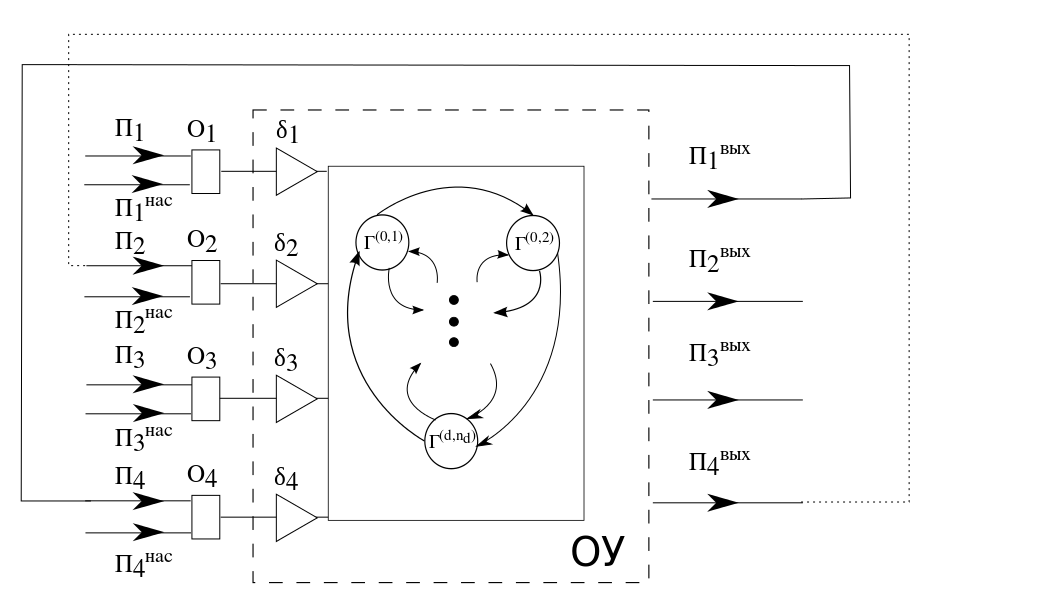
\includegraphics[scale=0.5]{SystemScheme.png} 
\caption{Структурная схема системы обслуживания}
\label{SystemScheme}
\end{figure}

Пусть в систему с одним обслуживающим устройством поступают потоки $\Pi_1$, $\Pi_2$, $\Pi_3$  и $\Pi_4$. Требования по потоку $\Pi_j$ становятся в соответствующую очередь $O_j$ с неограниченной вместимостью, $j\in \{1, 2, 3, 4\}$. Для $j \in \{1, 2, 3\}$ дисциплина очереди $O_j$, поддерживаемая устройством $\delta_j$, имеет тип FIFO (First In First Out). Таким образом, для обслуживания из соответствующей очереди выбирается то требование, которое пришло раньше. Дисциплина очереди $O_4$ будет описана ниже. Входные потоки $\Pi_1$ и $\Pi_3$ формируются внешней средой, которая, будем предполагать, имеет только одно состояние, то есть вероятностная структура потоков не меняется с течением времени. Требования потоков $\Pi_1$ и $\Pi_3$ формируют независимые между собой неординарные пуассоновские потоки, то есть  стационарные, без последействия и ординарные потоки групп требований. Интенсивности соответствующих простейших потоков для $\Pi_1$ и $\Pi_3$ будем обозначать $\lambda_1$ и $\lambda_3$, а распределение числа заявок в группе по потоку $\Pi_j$ будем описывать производящей функцией
\begin{equation}
f_j(z) = \sum_{\nu=1}^{\infty} p_{\nu}^{(j)} z ^{\nu}, \quad j\in \{1,3\},
\label{GeneratingFunc}
\end{equation}
которая предполагается аналитической при любом $z\in \mathbb{C}$ таком, что $|z|<(1+\varepsilon)$, $\varepsilon>0$. Величина $p_{\nu}^{(j)}$ определяет вероятность того, что по потоку $\Pi_j$ число требований в группе равно $\nu$. Обслуженные требования потока $\Pi_1$ поступают на повторное обслуживание, формируя на выходе поток $\Pi_4$. Обслуженные требования потока $\Pi_4$ в свою очередь поступают на повторное обслуживание, формируя при этом поток $\Pi_2$. Потоки $\Pi_2$ и $\Pi_3$ являются конфликтными, что означает запрет на одновременное обслуживание требований этих потоков и, следовательно, исследование системы не может быть сведено к задаче с меньшим числом потоков. 

В каждый момент времени обслуживающее устройство находится в одном из конечного множества состояний $\Gamma=\{\Gamma^{(k,r)} \colon k=\overline{0,d}; r=\overline{1,n_k}\}$ с заданными натуральными числами $d$, $n_0$, $n_1$, $\ldots$, $n_d$. В каждом состоянии $\Gamma^{(k,r)}$ обслуживающее устройство находится в течение времени $T^{(k,r)}$. Введем множества $\Gamma^{\mathrm{I}}$, $\Gamma^{\mathrm{II}}$, $\Gamma^{\mathrm{III}}$ и $\Gamma^{\mathrm{IV}}$ следующим образом. В состоянии $\gamma \in \Gamma^{\mathrm{\Rmnum{1}}}$ обслуживаются только требования из очередей $O_1$, $O_2$ и $O_4$.
В состоянии $\gamma \in \Gamma^{\mathrm{\Rmnum{2}}}$ обслуживаются только требования из очередей $O_2$ и $O_4$.
В состоянии $\gamma \in \Gamma^{\mathrm{\Rmnum{3}}}$ обслуживаются только требования из очередей $O_1$, $O_3$ и $O_4$.
В состоянии $\gamma \in \Gamma^{\mathrm{\Rmnum{4}}}$ обслуживаются только требования из очередей $O_3$ и $O_4$.
Тогда множество $\Gamma$ есть объединение $\Gamma = \Gamma^{\mathrm{I}} \cup \Gamma^{\mathrm{II}} \cup \Gamma^{\mathrm{III}} \cup \Gamma^{\mathrm{III}}$ непересекающихся подмножеств. Также в дальнейшем нам понадобятся множества ${}^1\Gamma=\Gamma^{\mathrm{\Rmnum{1}}} \cup \Gamma^{\mathrm{\Rmnum{3}}}$, 
${}^2\Gamma=\Gamma^{\mathrm{\Rmnum{1}}} \cup \Gamma^{\mathrm{\Rmnum{2}}}$,
${}^3\Gamma=\Gamma^{\mathrm{\Rmnum{3}}} \cup \Gamma^{\mathrm{\Rmnum{4}}}$. 

Смена состояний обслуживающего устройства осуществляется по следующему правилу. Множество состояний $C_k = \{\Gamma^{(k,r)} \colon r=\overline{1,n_k}\}$ будем называть $k$-м циклом, $k=\overline{1,d}$ (Рис. \ref{GraphScheme}). Состояние вида $\Gamma^{(0,r)}$ будем называть состоянием продления, $r=\overline{1,n_0}$. Положим $r \oplus_k 1 = r+1$ для $r=\overline{1,n_k-1}$ и $r \oplus_k 1 = 1$ при $r=n_k$, $k = \overline{0,d}$. В цикле $C_k$ выделим подмножества $C_k^{\mathrm{O}}$ выходных, $C_k^{\mathrm{I}}$ входных и $C_k^{\mathrm{N}} = C_k \setminus (C_k^{\mathrm{O}} \cup C_k^{\mathrm{I}})$ нейтральных состояний. Тогда после состояния $\Gamma^{(k,r)} \hm\in C_k\setminus C_k^{\mathrm{O}}$ обслуживающее устройство переходит в состояние $\Gamma^{(k,r \oplus_k 1)}$ того же цикла $C_k$. При $\Gamma^{(k,r)}$ принадлежащем множеству $C_k^{\mathrm{O}}$ прибор переходит в состояние $\Gamma^{(k,r \oplus_k 1)}$, если число требований в очереди $O_3$ в момент переключения больше заданного порога $L$. В противном случае, то есть если число требований в очереди $O_3$ меньше либо равно $L$, новое состояние прибора будет состоянием продления $\Gamma^{(0,r_1)}$, где $r_1=h_1(\Gamma^{(k,r)})$ и $h_1(\cdot)$~--- заданное отображение множества $\bigcup\limits_{k=1}^d C_k^{\mathrm{O}}$ во множество $\{1,2,\ldots, n_0\}$. После состояния $\Gamma^{(0,r)}$ выбирается состояние того же вида $\Gamma^{(0,r_2)}$, если число требований в очереди $O_3$ меньше или равно $L$, где $r_2=h_2(r)$ и $h_2(\cdot)$~--- заданное отображение множества $\{1,2, \ldots, n_0\}$ на себя; в противном случае включается входное состояние $\Gamma^{(k,r_3)} \in C_k^{\mathrm{I}}$, где $\Gamma^{(k,r_3)}=h_3(r)$ и $h_3(\cdot)$~--- заданное отображение множества $\{1,2, \ldots, n_0\}$ на множество  $\bigcup\limits_{k=1}^d C_k^{\mathrm{I}}$. Считается, что все состояния продления $\Gamma^{(0,r)}$ принадлежат множеству ${}^2 \Gamma$, а также верны соотношения $C_k^\mathrm{O}\subset {}^2 \Gamma$ и $C_k^\mathrm{I}\subset {}^3 \Gamma$. Также будем предполагать, что все циклы имеют ровно одно входное и одно выходное состояние. И последним предположением является то, что все вершины продления образуют один цикл, то есть можем положить $h_2(r)=r\oplus_0 1$.

\begin{figure}[hb]\centering
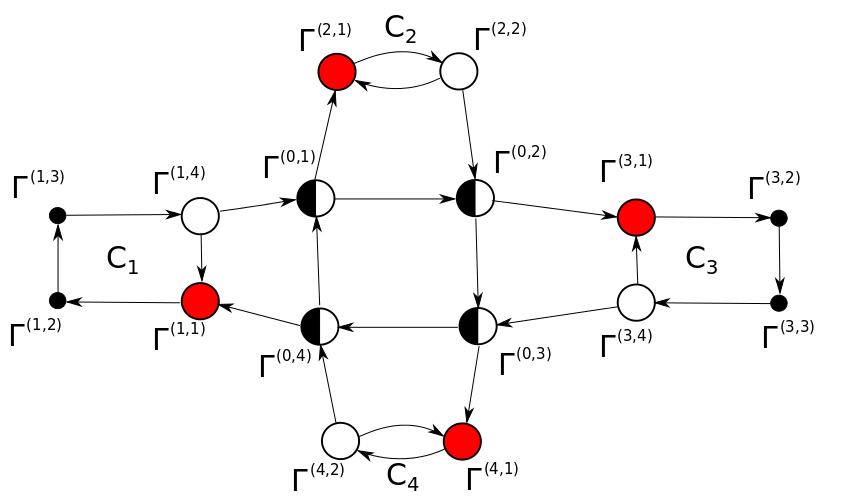
\includegraphics[scale=0.5]{GraphScheme3.png} 
\caption{Класс графов переходов. Незакрашенные вершины являются выходными вершинами, красным отмечены входные вершины, черным --- нейтральные, наполовину закрашенным вершинам соответствуют состояния продления}
\label{GraphScheme}
\end{figure}
%\subsection{Допустимые графы переходов состояний ОУ}

Таким образом, смена состояний обслуживающего устройства задается соотношением:
\begin{equation}
h(\Gamma^{(k,r)},y) = 
\begin{cases}
\Gamma^{(k,r \oplus_k 1)},& \quad \text{ если } (\Gamma^{(k,r)}\in C_k\setminus C_k^{\mathrm{O}}) \text{ или } (\Gamma^{(k,r)}\in C_k^{\mathrm{O}} \text{ \& } y>L);\\
%\Gamma^{(k,r \oplus_k 1)},& \quad \text{ если } \Gamma^{(k,r)}\in C_k^{\mathrm{O}} \text{ и } y>L;\\
\Gamma^{(0,h_1(\Gamma^{(k,r)}))},& \quad \text{ если } \Gamma^{(k,r)}\in C_k^{\mathrm{O}} \text{ и } y\leqslant L;\\
\Gamma^{(0,r \oplus_0 1)},& \quad \text{ если } k=0 \text{ и } y\leqslant L;\\
h_3(r),& \quad \text{ если } k=0 \text{ и } y > L.
\end{cases}
\label{hLaw}
\end{equation}

Рассмотрим введеные обозначения на примере рис.~\ref{GraphScheme}. Входными состояниями обслуживающего устройства являются $\Gamma^{(1,1)} \in C_1^{\mathrm{I}}$, $\Gamma^{(2,1)} \in C_2^{\mathrm{I}}$, $\Gamma^{(3,1)} \in C_3^{\mathrm{I}}$ и $\Gamma^{(4,1)} \in C_4^{\mathrm{I}}$, выходные состояния~--- $\Gamma^{(1,4)} \in C_1^{\mathrm{O}}$, $\Gamma^{(2,2)} \in C_2^{\mathrm{O}}$, $\Gamma^{(3,4)} \in C_3^{\mathrm{O}}$ и $\Gamma^{(4,2)} \in C_4^{\mathrm{O}}$, нейтральные состояния~--- $\Gamma^{(1,2)}, \Gamma^{(1,3)} \in C_1^{\mathrm{N}}$ и $\Gamma^{(3,2)}, \Gamma^{(3,3)} \in C_3^{\mathrm{N}}$. Состояния продления на графе представлены вершинами $\Gamma^{(0,1)}$, $\Gamma^{(0,2)}$, $\Gamma^{(0,3)}$ и $\Gamma^{(0,4)}$. Далее, отображение $h_1(\cdot)$ на графе задано таким образом, что оно переводит, например, выходное состояние $\Gamma^{(1,4)}$ в число $1$~--- номер состояния продления $\Gamma^{(0,1)}$, то есть $h_1(\Gamma^{(1,4)})=1$. Аналогично, например, $h_2(1)=2$ и $h_2(3)=4$. Примером отображения $h_3(\cdot)$ является $h_3(2)=\Gamma^{(3,1)}$.


Предполагается, что длительности обслуживания различных требований могут быть зависимыми и иметь различные законы распределения, поэтому вместо классического способа, состоящего в указании функции распределения длительности обслуживания произвольного требования, будут использованы потоки насыщения. Потоки насыщения $\Pi^{\mathrm{\text{нас}}}_j$, $j=\overline{1,4}$, определяются как виртуальные выходные потоки при условии максимального использования ресурсов обслуживающего устройства, а для $j=\overline{1,3}$ еще и при условии максимальной загрузки соответствующих очередей. 
Поток насыщения $\Pi^{\mathrm{\text{нас}}}_j$, $j=\overline{1,3}$, будет содержать неслучайное число $\ell(k,r,j)$ требований, обслуженных в течение времени $T^{(k,r)}$, если обслуживающее устройство находится в состоянии $\Gamma^{(k,r)}$. Пусть $\mathbb{Z}_+$~--- множество целых неотрицательных чисел. Тогда, при условии, что в очереди $O_4$ находится $x \in \mathbb{Z}_+$ требований, поток насыщения $\Pi^{\mathrm{\text{нас}}}_4$ определим как поток, содержащий все $x$ требований.
%\subsection{Пример: тандем из двух перекрестков} 
Наконец, при состоянии обслуживающего устройства $\Gamma^{(k,r)}$ каждое требование из очереди $O_4$ с вероятностью $p_{k,r}$ и независимо от других завершает обслуживание и отправляется в очередь $O_2$ потока~$\Pi_2$. С вероятностью $1-p_{k,r}$ требование очереди $O_4$ остается в ней до следующего такта. На следующем такте процесс повторяется.

В качестве наглядной физической интерпретации можно привести тандем из двух перекрестков (рис. \ref{crossroads}).
\begin{figure}[h]
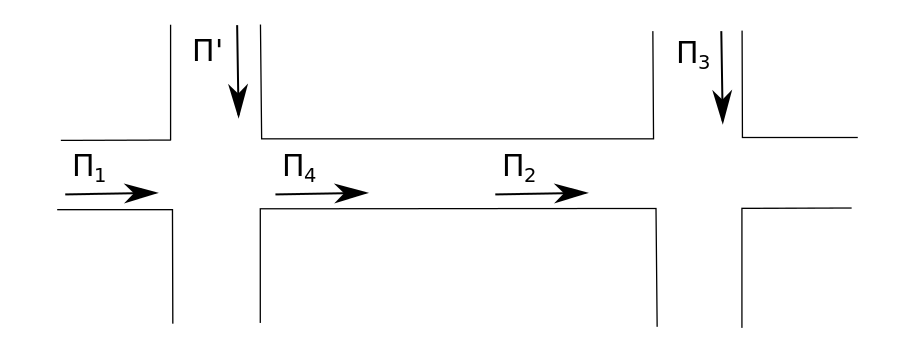
\includegraphics[scale=0.5]{Crossroads.png} 
\caption{Пример: тандем перекрестков}
\label{crossroads}
\end{figure}
В качестве потоков требований, формируемых внешней средой, выступают потоки прибывающих на перекрестки машин: конфликтные потоки $\Pi_1$, $\Pi_5$ на первом перекрестке, а также поток $\Pi_3$ на втором. Каждая машина из потока $\Pi_1$, проезжая первый перекресток, становится в очередь $O_4$ потока $\Pi_4$ и затем с некой вероятностью ($p_{k,r}$ для состояния $\Gamma^{(k,r)}$ обслуживающего устройства) доезжает до следующего перекрестка, или же не успевает это сделать и остается в очереди $O_4$ до следующего такта обслуживания. В случае, если машина из очереди $O_4$ успевает доехать до второго перекрестка, она становится в очередь $O_2$ и ждет своей очереди для его прохождения.

Предполагается, что светофор на первом перекрестке имеет лишь два состояния $\{g_{1,1},g_{1,2}\}$: в состоянии $g_{1,1}$ машины потока $\Pi_1$ пропускаются фиксированное количество времени $\widetilde T^{(1,1)}$ (<<зеленый>> свет для $\Pi_1$); в состоянии $g_{1,2}$ --- простаивают в течение времени $\widetilde T^{(1,2)}$ (<<красный>> свет для $\Pi_1$). Светофор на втором перекрестке обслуживает по алгоритму с продлением: дополнительно к состоянию обслуживания потока $\Pi_3$ (состояние $g_{2,1}$), также имеется два состояния обслуживания потока $\Pi_2$ (состояния $\{g_{2,2},g_{2,3}\}$). Первое из них включается всегда после завершения обслуживания потока $\Pi_3$, а второе включается, если после очередного такта обслуживания потока $\Pi_2$ длина очереди $O_3$ не превосходит уровня $L$.
Длительности пребывания светофора на втором перекрестке в каждом из состояний суть $\widetilde T^{(2,1)}$, $\widetilde T^{(2,2)}$ и $\widetilde T^{(2,3)}$.


Рассматривая тандем из двух перекрестков как единую систему массового обслуживания и предполагая наблюдение за ней только в (дискретные) моменты переключения состояния хотя бы одного из светофоров, может быть показано, что количество различных состояний у полученной системы конечно. Действительно, положим, например, за состояние объединенной системы вектор $(g^{(1)},g^{(2)}, s, t)$, где $g^{(1)}\in \{g_{1,1},g_{1,2}\}$~--- состояние $1$--го перекрестка, $g^{(2)}\in \{g_{2,1},g_{2,2},g_{2,3}\}$~--- состояние $2$--го перекрестка, $s \in \{0, 1, 2\}$~--- номер последнего сменившего состояние перекрестка (принимает значение $0$ в случае, если сменили состояние оба перекрестка) и $t \in \{0, 1, 2, \ldots, T\}$~--- количество времени, оставшееся у продолжающего обслуживание с прошлого такта перекрестка (принимает значение $0$, если принимает значение $0$ величина $s$). Здесь $T$~--- максимальная длительность нахождения каждого из светофоров в одном состоянии. Тогда количество различных состояний не трудно посчитать и оно не будет превышать величины  $2\times 3 \times 3 \times T$.

В завершение построения примера отметим, что при прохождении перекрестков машины предполагаются движущимися только в прямом направлении, то есть перемешивания конфликтных потоков не допускается. Таким образом, поток $\Pi_5$ не представляет интереса для дальнейшего исследования системы и может быть отброшен и, следовательно, построенный пример целиком удовлетворяет структурной схеме на рис. \ref{SystemScheme}.

Теперь продемонстрируем на конкретном числовом примере выделение циклов и состояний продления. Пусть изменение состояний перекрестков и время пребывания (в секундах для определнности) в каждом из состояний задается графами на рис. \ref{SystemStates}.
\begin{figure}[h]
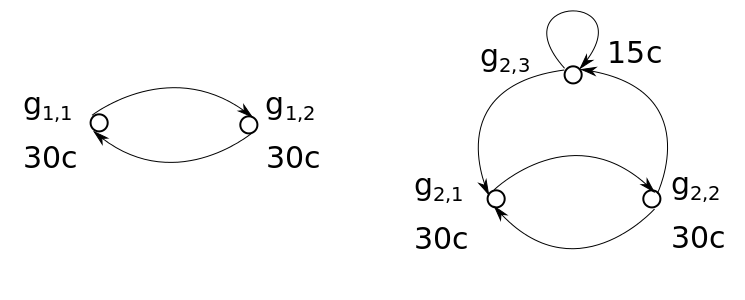
\includegraphics[scale=0.5]{SystemStates.png} 
\caption{Числовой пример тандема перекрестков. Левый граф соответствует первому перекрестку, правый~--- второму}
\label{SystemStates}
\end{figure}
За начальное состояние объединенной системы примем $\Gamma_0=(g_{1,1},g_{2,1},0,0)$, то есть первый перекресток находится в состоянии $g_{1,1}$, второй~--- в состоянии $g_{2,1}$, и оба только начали свою работу в своем состоянии (этот факт моделируется равенствами $s=0$ и $t=0$). Следующая смена состояний случится у обоих перекрестков одновременно и приведет к следующему состоянию $(g_{1,2},g_{2,2}, 0, 0)$. Далее смена состояний произойдет также у первого и второго перекрестков, однако второй перекресток может перейти как в состояние $g_{2,1}$, так и в состояние продления $g_{2,3}$. Таким образом следущим состоянием тандема будет либо опять $(g_{1,1},g_{2,1},0,0)$, либо $(g_{1,1},g_{2,3},0,0)$. Продолжая рассуждения аналогичным образом, получим следущий список всех возможных состояний системы:
\begin{align*}
(g_{1,1},g_{2,1},0,0)&=\Gamma^{(1,1)} ,& \quad (g_{1,2},g_{2,2},0,0)&=\Gamma^{(1,2)} ,& \quad (g_{1,1},g_{2,3},0,0)&=\Gamma^{(0,1)}, \\
(g_{1,1},g_{2,3},15,2)&=\Gamma^{(0,2)} ,& \quad (g_{1,2},g_{2,3},0,0)&=\Gamma^{(0,3)} ,& \quad (g_{1,2},g_{2,3},15,2)&=\Gamma^{(0,4)}, \\
(g_{1,2},g_{2,1},15,2)&=\Gamma^{(4,1)} ,& \quad (g_{1,1},g_{2,1},15,1)&=\Gamma^{(4,2)} ,& \quad (g_{1,1},g_{2,2},15,2)&=\Gamma^{(4,3)}, \\
(g_{1,2},g_{2,2},15,1)&=\Gamma^{(4,4)} ,& \quad (g_{1,2},g_{2,3},15,2)&=\Gamma^{(0,5)} ,& \quad (g_{1,2},g_{2,1},0,0)&=\Gamma^{(3,1)}, \\
(g_{1,1},g_{2,2},0,0)&=\Gamma^{(3,2)} ,& \quad (g_{1,1},g_{2,1},15,2)&=\Gamma^{(2,1)} ,& \quad (g_{1,2},g_{2,1},15,1)&=\Gamma^{(2,2)}, \\
(g_{1,2},g_{2,2},15,2)&=\Gamma^{(2,3)} ,& \quad (g_{1,1},g_{2,2},15,1)&=\Gamma^{(2,4)}. & &
\end{align*}
В соответсвии с приведенными выше обозначениями, множества $C_1$, $C_2$, $C_3$, $C_4$, а также множество состояний продления строятся однозначным образом. Множествами входных состояний будут $C_1^{\mathrm{I}}=\{\Gamma^{(1,1)}\}$, $C_2^{\mathrm{I}}=\{\Gamma^{(2,1)}\}$, $C_3^{\mathrm{I}}=\{\Gamma^{(3,1)}\}$ и $C_4^{\mathrm{I}}=\{\Gamma^{(4,1)}\}$. Множествами выходных состояний будут $C_1^{\mathrm{O}}=\{\Gamma^{(1,2)}\}$, $C_2^{\mathrm{O}}=\{\Gamma^{(2,4)}\}$, $C_3^{\mathrm{O}}=\{\Gamma^{(3,2)}\}$ и $C_4^{\mathrm{O}}=\{\Gamma^{(4,4)}\}$. Функции $h_1(\cdot)$, $h_2(\cdot)$ и $h_3(\cdot)$ задаются поточечно:
\begin{equation*}
h_1(\Gamma^{(1,2)})=1, \quad h_1(\Gamma^{(2,4)})=2, \quad h_1(\Gamma^{(3,2)})=3, \quad h_1(\Gamma^{(4,4)})=5,
\end{equation*}
\begin{equation*}
h_2(1)=2, \quad h_2(2)=3, \quad h_2(3)=4 \quad h_2(4)=1, \quad h_2(5)=1,
\end{equation*}
\begin{equation*}
h_3(1)=\Gamma^{(2,1)}, \quad h_3(2)=\Gamma^{(3,1)}, \quad h_3(3)=\Gamma^{(4,1)} \quad h_3(4)=\Gamma^{(1,1)}, \quad h_3(5)=\Gamma^{(1,1)}.
\end{equation*}
Этим завершается построение числового примера.

\subsection{Представление рассматриваемой системы обслуживания в виде кибернетической управляющей системы}
Описанная в предыдущем разделе на содержательном уровне система массового обслуживания должна рассматриваться как кибернетическая управляющая система обслуживания (см. \cite{Zorine:2011}). Схема управляющей системы приведена на рис. \ref{SystemScheme}. На схеме присутствуют следующие блоки: 1) внешняя среда с одним состоянием; 2) входные полюса первого типа~--- входные потоки $\Pi_1$, $\Pi_2$, $\Pi_3$, $\Pi_4$; 3) входные полюса второго типа~--- потоки насыщения $\Pi_1^{\mathrm{\text{нас}}}$, $\Pi_2^{\mathrm{\text{нас}}}$, $\Pi_3^{\mathrm{\text{нас}}}$, $\Pi_4^{\mathrm{\text{нас}}}$; 4) внешняя память~--- очереди $O_1$, $O_2$, $O_3$, $O_4$; 5) устройство по переработкe информации внешней памяти~--- устройства по поддержанию дисциплины очереди $\delta_1$, $\delta_2$, $\delta_3$, $\delta_4$; 6) внутренняя память~--- обслуживающее устройство (ОУ); 7) устройство по переработке информации во внутренней памяти~--- граф смены состояний; 8) выходные полюса $\Pi_1^{\mathrm{\text{вых}}}$, $\Pi_2^{\mathrm{\text{вых}}}$, $\Pi_3^{\mathrm{\text{вых}}}$, $\Pi_4^{\mathrm{\text{вых}}}$. Координатой блока является номер этого блока на схеме. 

Для задания информации блоков введем следующие величины и элементы, а также укажем множества их возможных значений. В качестве дискретной временной шкалы выберем последовательность $\tau_0=0$, $\tau_1$, $\tau_2$, $\ldots$ моментов смены состояния обслуживающего устройства. Обозначим $\Gamma_i$, $i\geqslant 1$, из множества $\Gamma$ состояние обслуживающего устройства в течение времени $\left(\tau_{i-1};\tau_i\right]$ и $\Gamma_0\in \Gamma$~--- в момент времени $\tau_0$, количество $\varkappa_{j,i} \in \mathbb{Z}_+ $, $i\geqslant 0$, требований в очереди $O_j$ в момент времени $\tau_i$, количество $\eta_{j,i} \in \mathbb{Z}_+$, $i\geqslant 0$, требований, поступивших в очередь $O_j$ по потоку $\Pi_j$ в течение времени $\left(\tau_{i};\tau_{i+1}\right]$, количество $\xi_{j,i} \in \mathbb{Z}_+$, $i\geqslant 0$, требований по потоку насыщения $\Pi^{\mathrm{\text{нас}}}_j$ в течение времени $\left(\tau_{i};\tau_{i+1}\right]$, количество $\overline{\xi}_{j,i}\in \mathbb{Z}_+$, $i\geqslant 0$, реально обслуженных требований по потоку $\Pi_j$ в течение времени $\left(\tau_{i};\tau_{i+1}\right]$; $j=\overline{1,4}$.

Закон изменения состояния обслуживающего устройства будем предполагать заданным соотношением 
\begin{equation}
\Gamma_{i+1}=h(\Gamma_i,\varkappa_{3,i}),
\label{gammaFunc}
\end{equation}
где отображение $h(\cdot,\cdot)$ определено в \eqref{hLaw}.
Для определения длительности $T_{i+1}$ состояния обслуживающего устройства в течение времени $\left(\tau_{i};\tau_{i+1}\right]$ удобно ввести функцию $h_T(\cdot,\cdot)$:
\begin{equation*}
T_{i+1}=h_T(\Gamma_i,\varkappa_{3,i})= T^{(k,r)},\quad  \text{ где $k$ и $r$ таковы, что } \Gamma^{(k,r)}=\Gamma_{i+1}=h(\Gamma_i,\varkappa_{3,i}).
%\label{timeLaw}
\end{equation*}
Функциональная зависимость
\begin{equation}
\overline{\xi}_{j,i}=\min\{\varkappa_{j,i}+\eta_{j,i},\xi_{j,i}\}, \quad j\in \{1,2,3\},
\label{saturationEq}
\end{equation}
между величиной $\overline{\xi}_{j,i}$ и величинами $\varkappa_{j,i}$, $\eta_{j,i}$, $\xi_{j,i}$ реализует стратегию механизма обслуживания требований. Далее, поскольку 
\begin{equation*}
\varkappa_{j,i+1}=\varkappa_{j,i}+\eta_{j,i}-\overline{\xi}_{j,i}, \quad  j\in \{1,2,3\},
\end{equation*}
то из \eqref{saturationEq} следует соотношение
\begin{equation}
\varkappa_{j,i+1}=\max\{{0,\varkappa_{j,i}+\eta_{j,i}-\xi_{j,i}}\}, \quad j\in \{1,2,3\}.
\label{queuesFunc}
\end{equation}
Из формулировки поставленной задачи (см. также структурную схему на рис.~\ref{SystemScheme}) следуют соотношения для потока $\Pi_4$:
\begin{equation}
\eta_{4,i} = \min\{\xi_{1,i}, \varkappa_{1,i}+\eta_{1,i}\}, \quad \varkappa_{4,i+1}=\varkappa_{4,i}+\eta_{4,i}-\eta_{2,i}, \quad \xi_{4,i} = \varkappa_{4,i}.
\label{FourthFunc}
\end{equation}

Нелокальное описание входных потоков и потоков насыщения состоит в указании некоторых свойств условных распределений выделенных дискретных компонент $\eta_i=(\eta_{1,i},\eta_{2,i}, \eta_{3,i}, \eta_{4,i})$ и $\xi_i=(\xi_{1,i}, \xi_{2,i}, \xi_{3,i}, \xi_{4,i})$ маркированных точечных процессов \linebreak $\{(\tau_i, \nu_i, \eta_i); i\geqslant 0\}$ и $\{(\tau_i, \nu_i, \xi_i); i\geqslant 0\}$ при фиксированных значениях метки $\nu_i = (\Gamma_i;\varkappa_i)$, где $\varkappa_i=(\varkappa_{1,i},\varkappa_{2,i},\varkappa_{3,i},\varkappa_{4,i})$. 
Введем функции $\varphi_1(\cdot,\cdot)$ и $\varphi_3(\cdot,\cdot)$ из разложений 
\begin{equation*}
\sum_{\nu=0}^{\infty} z^\nu\varphi_j(\nu,t) = \exp\{\lambda_j t (f_j(z)-1)\},
\end{equation*}
где $f_j(z)$ определены в \eqref{GeneratingFunc}, $j \in \{1,3\}$. Функция $\varphi_j(\nu,t)$ по своему смыслу есть вероятность поступления $\nu=0$, $1$, $\ldots$ требований по потоку $\Pi_j$ за время $t \geqslant 0$. Положим $\varphi_j(\nu,t)$ равной нулю при $\nu < 0$. Функцию $\psi(\cdot,\cdot,\cdot)$ зададим формулой
\begin{equation*}
\psi(k;y,u)=C_y^k u^k (1-u)^{y-k}.	
\end{equation*}
По своему смыслу $\psi(k;y,u)$ есть вероятность поступления $k$ требований по потоку $\Pi_2$ при условии, что очередь $O_4$ содержит $y$ требований и обслуживающее устройство находится в состоянии $\Gamma^{(k,r)}$, так что $u=p_{k,r}$. При нарушении условия $ 0\leqslant k \leqslant y$ положим $\psi(k;y,u)$ равной нулю.

Пусть $a=(a_1, a_2, a_3, a_4) \in \mathbb{Z}_+^4$ и $x=(x_1, x_2, x_3, x_4) \in \mathbb{Z}_+^4$. Тогда из постановки задачи на содержательном уровне следует, что при фиксированном значении метки $\nu_i=(\Gamma^{(k,r)}; x)$ вероятность $\varphi(a,k,r,x)$ одновременного выполнения равенств $\eta_{1,i}=a_1$, $\eta_{2,i}=a_2$, $\eta_{3,i}=a_3$, $\eta_{4,i}=a_4$ есть 
\begin{equation}
\varphi_1(a_1,h_T(\Gamma^{(k,r)},x_3)) \times \psi(a_2,x_4, p_{\tilde{k},\tilde{r}}) \times \varphi_3(a_3,h_T(\Gamma^{(k,r)},x_3))
\times \delta_{a_4,\min{\{\ell(\tilde{k},\tilde{r},1), x_1+a_1}\}},
\label{conditionProbOne}
\end{equation}
где $\tilde{k}$ и $\tilde{r}$ таковы, что $\Gamma^{(\tilde{k},\tilde{r})}=h(\Gamma^{(k,r)},x_3)$ и $\delta_{i,j}$ есть символ Кронекера
\begin{equation*}
\delta_{i,j}=\begin{cases} 1, \quad \text{ если }i=j\\0, \quad \text{ если } i\neq j,
\end{cases}.
\end{equation*}
Пусть $b=(b_1, b_2, b_3, b_4) \in \mathbb{Z}_+^4$. Из содержательной постановки задачи также следует, что вероятность $\zeta(b, k, r, x)$ одновременного выполнения равенств $\xi_{1,i}=b_1$, $\xi_{2,i}=b_2$, $\xi_{3,i}=b_3$, $\xi_{4,i}=b_4$ при фиксированном значении метки $\nu_i=(\Gamma^{(k,r)}; x)$ есть
\begin{equation}
\delta_{b_1,\ell(\tilde{k},\tilde{r},1)} \times \delta_{b_2,\ell(\tilde{k},\tilde{r},2)} \times 
\delta_{b_3,\ell(\tilde{k},\tilde{r},3)} \times \delta_{b_4,x_4}.
\label{conditionProbTwo}
\end{equation}
Из формулы \eqref{conditionProbTwo} следует для $j\in \{1, 2, 3\}$, что вероятность события $\xi_{j,i}=0$ равна $1$ в случае $h(\Gamma^{(k,r)},x_3)\notin {}^j\Gamma$ и что вероятность события $\xi_{j,i}=\ell(\tilde{k},\tilde{r},j)$ равна $1$, если $\Gamma^{(\tilde{k},\tilde{r})}=h(\Gamma^{(k,r)},x_3)\in {}^j\Gamma$.


Содержательный смысл следующей теоремы состоит в том, что сформулированные выше функциональные связи и вероятностные свойства введенных объектов непротиворечивы и могут быть реализованы на некотором общем вероятностном пространстве.
%Построим теперь 	вероятностное пространство $(\Omega, {\cal F}, \Pr(\cdot))$, чтобы можно было рассматривать введеные величины как случайные величины на этом пространстве. А именно, докажем следующую теорему.
\begin{theorem}
Пусть $\gamma_0=\Gamma^{(k_0,r_0)}\in \Gamma$ и $x^0=(x_{1,0},x_{2,0}, x_{3,0},x_{4,0})\in \mathbb{Z}_+^4$ фиксированы.
Тогда существует вероятностное пространство $(\Omega, {\cal F}, \Pr(\cdot))$ и заданные на нем случайные величины $\eta_{j,i}=\eta_{j,i}(\omega)$, $\xi_{j,i}=\xi_{j,i}(\omega)$, 	 $\varkappa_{j,i}=\varkappa_{j,i}(\omega)$ и случайные элементы $\Gamma_i=\Gamma_i(\omega)$, $i\geqslant 0$, $j\in \overline{1,4}$, такие, что 1) имеют место равенства $\Gamma_0(\omega) = \gamma_0$ и $\varkappa_0(\omega)=x^0$; 2) выполняются соотношения \eqref{gammaFunc}, \eqref{queuesFunc}, \eqref{FourthFunc}; 3) для любых  $a$, $b$, $x^t=(x_{1,t},x_{2,t},x_{3,t},x_{4,t}) \in \mathbb{Z}_+^4$, $\Gamma^{(k_t,r_t)} \in \Gamma$, $t = 1, 2, \ldots$, условное распределение векторов $\eta_i$, и $\xi_i$ имеет вид
\begin{equation}
\Pr \left(\{ \omega \colon \eta_i = a, \xi_i=b\} \left|\bigcap_{t=0}^{i}\{\omega\colon \Gamma_t=\Gamma^{(k_t,r_t)}, \varkappa_t=x^t\}\right.\right)=
\varphi(a,k_i,r_i,x^i)\times \zeta(b,k_i,r_i,x^i),
\label{ProbablititiesToProve}
\end{equation}
где функции $\varphi(\cdot, \cdot, \cdot, \cdot)$ и $\zeta(\cdot, \cdot, \cdot, \cdot)$ определяются формулами \eqref{conditionProbOne} и \eqref{conditionProbTwo} соответственно, $i \geqslant 0$.

\label{myTheorem}
\end{theorem}
\begin{proof}
В соответствии с теоремой Ионеску Тулчи (см. \cite{Shiryaev}, c. 348--351) для доказательства достаточно задать на $(\Omega_0, {\cal F}_0)$ вероятностную меру $P_0(\cdot)$ и далее, считая для $0 < i \leqslant n$ и каждого набора элементарных исходов $(\omega_0, \omega_1, \ldots, \omega_{i-1})$ заданной на $(\Omega_i, {\cal F}_i)$ вероятностную меру $P(\omega_0,\omega_1,\ldots, \omega_{i-1};\cdot)$, задать на $(\Omega_{n+1}, {\cal F}_{n+1})$ меру $P(\omega_0,\omega_1,\ldots, \omega_{n};\cdot)$, причем для любого множества $B\in {\cal F}_i$ функции $P(\omega_0,\omega_1,\ldots, \omega_{i-1};B)$
должны быть измеримыми функциями от $(\omega_0, \omega_1, \ldots, \omega_{i-1})$. Тогда для декартова произведения пространств элементарных исходов $\Omega=\prod\limits_{i=0}^{\infty}\Omega_i$ и произведения $\sigma$-алгебр ${\cal F}=\bigotimes\limits_{i=0}^{\infty} {\cal F}_i$ на $(\Omega,{\cal F})$ будет существовать единственная вероятностная мера $\Pr(\cdot)$ такая, что для любого $i \geqslant 0$ верно равенство
\begin{equation}
\Pr\{\omega \colon \omega_0 \in A_0, \omega_1 \in A_1, \ldots, \omega_i\in A_i\} = P_i(A_0 \times A_1 \times \ldots \times A_i),
\label{ProbabilitiesGeneral}
\end{equation}
где 
\begin{equation}
 P_i(A_0 \times A_1 \times \ldots \times A_i) = \int_{A_0} P_0(d \omega_0) \int_{A_1} P(\omega_0;d \omega_1) \ldots \int_{A_i} P(\omega_0, \omega_1, \ldots, \omega_{i-1}; d \omega_i),
\label{ProbabilitiesGeneralOne}
\end{equation}
для любого $A_i$ из ${\cal F}_i$. 

Итак, за описание элементарного исхода $\omega_i \in \Omega_i$ для произвольного $i \geqslant 0$ примем набор $(\omega_{1,i},\omega_{2,i},\omega_{3,i})$, $\omega_{j,i}\in \mathbb{Z}_+$. Таким образом, $\Omega_i=\mathbb{Z}_+^3$ и в качестве $\sigma$-алгебры ${\cal F}_i$ возьмем множество всех подмножеств множества $\Omega_i$: ${\cal F}_i=2^{\Omega_i}$. Пусть $\Gamma^{(\tilde{k},\tilde{r})}=h(\Gamma^{(k_0,r_0)},x_{3,0})$. Тогда,  поскольку множество $\Omega_0$ счетно, определим вероятностную меру $P_0(\cdot)$ на измеримом пространстве $(\Omega_0,{\cal F}_0)$ ее значениями на одноточечных множествах:
\begin{equation}
P_0(\{(a_1,a_2,a_3)\})=\varphi_1(a_1,h_T(\Gamma^{(k_0,r_0)})) \times \psi(a_2,x_{2,0}, p_{\tilde{k},\tilde{r}}) \times \varphi_3(a_3,h_T(\Gamma^{(k_0,r_0)})).
\label{probabilitiesOne}
\end{equation}
Для $j\in \{1,2,3\}$ определим величины
\begin{equation}
\Gamma_0=\gamma_0, \quad \varkappa_{j,0}=x_{j,0}, \quad \xi_{j,0}=l(\tilde{k},\tilde{r},j), \quad \eta_{j,0}=\omega_{j,0},
\label{startRekOne}
\end{equation}
и
\begin{equation}
 \varkappa_{4,0}=x_{4,0}, \quad \xi_{4,0}=x_{4,0}, \quad \eta_{4,0}=\min\{\xi_{1,0}, x_{1,0}+\eta_{1,0}\}.
\label{startRekTwo}
\end{equation}

Теперь, предполагая заданными на $(\Omega_i, {\cal F}_i)$ вероятностные меры $P(\omega_0, \omega_1, \ldots, \omega_{i-1};\cdot)$, заданными величины $\Gamma_i$, $\varkappa_{j,i}$, $\xi_{j,i}$, $\eta_{j,i}$, $i=\overline{1,n}$, $j=\overline{1,4}$, и фиксируя набор $(\omega_0, \omega_1, \ldots, \omega_{n})$, определим на измеримом пространстве $(\Omega_{n+1}, {\cal F}_{n+1})$ меру $P(\omega_0, \omega_1, \ldots, \omega_n;\cdot)$. Положим для $j\in \{1, 2, 3\}$
\begin{equation}
\Gamma_{n+1}=\Gamma^{(k^*,r^*)}=h(\Gamma_{n},\varkappa_{3,n}), \quad \varkappa_{j,n+1}=\max\{ 0,\varkappa_{j,n}+\eta_{j,n} -\xi_{j,n}\},
\label{NextRekOne}
\end{equation}
\begin{equation}
\varkappa_{4,n+1}=\varkappa_{4,n}+\eta_{4,n}-\eta_{2,n}, \quad \xi_{j,n+1}=l(k^*,r^*,j),
\label{NextRekTwo}
\end{equation}
\begin{equation}
\eta_{j,n+1}=\omega_{j,n+1}, \quad \eta_{4,n+1}=\min\{\xi_{1,n+1}, \varkappa_{1,n+1}+\eta_{1,n+1}\}, \quad \xi_{4,n+1}=\varkappa_{4,n+1}.
\label{NextRekThree}
\end{equation}
Тогда, по аналогии с построением вероятностной меры $P_0(\cdot)$, зададим меру $P(\omega_0,\omega_1,\ldots,\omega_n;\cdot)$ на одноточечных множествах $\{(a_1,a_2,a_3)\}$, $(a_1,a_2,a_3)\in {\mathbb Z}_+^3$:
\ml
{
P(\omega_0,\omega_1,\ldots,\omega_n;\{(a_1,a_2,a_3)\}) = \\
= \varphi_1(a_1,h_T(\Gamma_n,x_{3,n})) \times \psi(a_2,x_{4,n}, p_{k^*,r^*}) \times \varphi_3(a_3,h_T(\Gamma_n,x_{3,n})).
\label{probabilitiesTwo}
}
Вероятностное пространство $(\Omega,{\cal F},\Pr(\cdot))$ построено. 

Теперь докажем, что введеные с помощью формул \eqref{startRekOne}~--~\eqref{NextRekThree} случайные элементы $\Gamma_i(\omega)$ и случайные величины $\varkappa_{j,i}(\omega)$, $\eta_{j,i}(\omega)$, $\xi_{j,i}(\omega)$, $i \geqslant 0$, $j =\overline{1,4}$ удовлетворяют условиям теоремы. Из формулы \eqref{NextRekOne} следует, что случайные элементы $\Gamma_i$ удовлетворяют соотношению \eqref{gammaFunc}, а случайные величины $\varkappa_{j,i}$ для $j\in \{1, 2, 3\}$ удовлетворяют соотношению \eqref{queuesFunc}. Из формулы \eqref{NextRekTwo} заключаем, что $\varkappa_{4,i}$ удовлетворяет соотношению $\eqref{FourthFunc}$. Далее, из \eqref{startRekTwo} и \eqref{NextRekThree} следует справедливость соотношений \eqref{FourthFunc} для величин $\eta_{4,i}$ и $\xi_{4,i}$. 

Перейдем к доказательству равенства \eqref{ProbablititiesToProve}. Для этого найдем явное выражение для условной вероятности $\Pr (\{ \omega \colon \eta_i = a, \xi_i=b\} | \bigcap_{t=0}^{i}\{\omega\colon \Gamma_t=\Gamma^{(k_t,r_t)}, \varkappa_t=x^t\})$. Пусть $\Gamma^{(\tilde{k}_i,\tilde{r}_i)}=h(\Gamma^{(k_i,r_i)},x^i)$. Распишем по определению условной вероятности:
\begin{multline}
\Pr \left(\left\{ \omega \colon \eta_i = a, \xi_i=b\right\}  \left| \bigcap_{t=0}^{i}\left\{\omega\colon \Gamma_t=\Gamma^{(k_t,r_t)}, \varkappa_t=x^t\right\}\right.\right) = \\
=\Pr\left(\{ \omega \colon \eta_i = a, \xi_i=b \} \cap \bigcap_{t=0}^{i}\{\omega\colon \Gamma_t=\Gamma^{(k_t,r_t)}, \varkappa_t=x^t\}\right) \Big/ \\
\Big/
\Pr\left( \bigcap_{t=0}^{i}\{\omega\colon \Gamma_t=\Gamma^{(k_t,r_t)}, \varkappa_t=x^t\}\right).
\label{Construction:1}
\end{multline}
Далее из \eqref{ProbabilitiesGeneral}, \eqref{ProbabilitiesGeneralOne} и того факта, что $\Gamma_i$ и $\varkappa_{i}$ зависят только от $\omega_0$, $\omega_1$ , $\ldots$, $\omega_{i-1}$, но не от $\omega_i$, (этот факт следует из формул \eqref{startRekOne}~--~\eqref{NextRekTwo}), получим выражение для знаменателя последней дроби
\begin{multline}
\Pr\left( \bigcap_{t=0}^{i}\{\omega\colon \Gamma_t=\Gamma^{(k_t,r_t)}, \varkappa_t=x^t\}\right)=\\
=\sum_{\substack{\omega_0, \omega_1,\ldots \omega_{i-1} \colon \\ \Gamma_t=\Gamma^{(k_t,r_t)}, \varkappa_t=x^t, \forall 0\leqslant t \leqslant i-1}} P_0(\omega_0)\times P(\omega_0;\{\omega_1\})\times\ldots\times P(\omega_0,\omega_1,\ldots, \omega_{i-2};\{\omega_{i-1}\}).
\label{Construction:2}
\end{multline}
Здесь мы положили $A_t(\omega_0,\omega_1,\ldots,\omega_{t-1})=\{\omega_t \colon \Gamma_t=\Gamma^{(k_t,r_t)}, \varkappa_t=x^t\}$, $t=\overline{0,i}$.

Преобразуем множество $\{ \eta_i = a, \xi_i=b \} \cap \{\Gamma_i=\Gamma^{(k_i,r_i)}, \varkappa_i=x^i\}$, учитывая соотношения \eqref{startRekOne}~--~\eqref{NextRekThree}:
\begin{multline*}
\left\{ \eta_i = a, \xi_i=b \right\} \cap \left\{\Gamma_i=\Gamma^{(k_i,r_i)}, \varkappa_i=x^i\right\} = \left\{\Gamma_i=\Gamma^{(k_i,r_i)}, \varkappa_i=x^i\right\} \cap\\
\cap \left\{ \eta_{j,i} = a_j, j=\overline{1,3}\right\} \cap \left\{ \xi_{j,i} = b_j, j=\overline{1,3}\right\} \cap \left\{ \xi_{4,i} = b_4 \right\} \cap  \left\{ \eta_{4,i} = a_4 \right\} = \\
= \left\{\Gamma_i=\Gamma^{(k_i,r_i)}, \varkappa_i=x^i\right\} \cap \left\{ \omega_{j,i} = a_j, j= \overline{1,3}\right\} \cap \left\{ b_j=\ell(\tilde{k}_i,\tilde{r}_i,j), j=\overline{1,3}\right\} \cap \\ 
\cap \left\{ b_4 = x_{4,i} \right\} \cap  \left\{ a_4=\min\left\{\ell(\tilde{k}_i,\tilde{r}_i,1), x_{1,i}+a_1\right\} \right\}. 
\end{multline*}
Тогда для числителя дроби из \eqref{Construction:1} имеем:
\begin{multline}
\Pr\left(\{ \omega \colon \eta_i = a, \xi_i=b \} \cap \bigcap_{t=0}^{i}\{\omega\colon \Gamma_t=\Gamma^{(k_t,r_t)}, \varkappa_t=x^t\}\right)=\\
= \Pr\left(\left\{ \eta_i = a, \xi_i=b \right\} \cap \left\{\Gamma_i=\Gamma^{(k_i,r_i)}, \varkappa_i=x^i\right\} \cap \bigcap_{t=0}^{i-1}\{\omega\colon \Gamma_t=\Gamma^{(k_t,r_t)}, \varkappa_t=x^t\}\right)=\\
= \delta_{b_4,x_{4,i}} \times \delta_{a_4,\min\left\{\ell(\tilde{k}_i,\tilde{r}_i,1), x_{1,i}+a_1\right\}} \times \prod_{j=1}^3\delta_{b_j,\ell(\tilde{k}_i,\tilde{r}_i,j)}   \times \\
\times \Pr\left( \left\{ \omega_{j,i} = a_j, j=\overline{1,3}\right\} \cap \left\{\Gamma_i=\Gamma^{(k_i,r_i)}, \varkappa_i=x^i\right\} \cap \bigcap_{t=0}^{i-1}\{\omega\colon \Gamma_t=\Gamma^{(k_t,r_t)}, \varkappa_t=x^t\}\right).
\label{Construction:3}
\end{multline}
И по аналогии со знаменателем (выражение \eqref{Construction:2}), распишем последнюю вероятность:
\begin{multline*}
\Pr\left( \left\{ \omega_{j,i} = a_j, j\in \{1, 2, 3\}\right\} \cap \left\{\Gamma_i=\Gamma^{(k_i,r_i)}, \varkappa_i=x^i\right\} \cap \bigcap_{t=0}^{i-1}\{\omega\colon \Gamma_t=\Gamma^{(k_t,r_t)}, \varkappa_t=x^t\}\right) =\\
= \sum_{\substack{\omega_0, \omega_1,\ldots \omega_{i-1} \colon \\ \Gamma_t=\Gamma^{(k_t,r_t)}, \varkappa_t=x^t, \forall 0\leqslant t \leqslant i-1}} P_0(\omega_0)\times P(\omega_0;\{\omega_1\})\times\ldots\times P(\omega_0,\omega_1,\ldots, \omega_{i-2};\{\omega_{i-1}\})\times\\
\times  P(\omega_0,\omega_1,\ldots, \omega_{i-1};\{(a_1, a_2, a_3)\})
\end{multline*}
и, учитывая выражение \eqref{probabilitiesTwo}, получим
\begin{multline}
\Pr\left( \left\{ \omega_{j,i} = a_j, j\in \{1, 2, 3\}\right\} \cap \left\{\Gamma_i=\Gamma^{(k_i,r_i)}, \varkappa_i=x^i\right\} \cap \bigcap_{t=0}^{i-1}\{\omega\colon \Gamma_t=\Gamma^{(k_t,r_t)}, \varkappa_t=x^t\}\right) =\\
=\varphi_1(a_1,h_T(\Gamma_i,x_{3,i})) \times \psi(a_2,x_{4,i}, p_{\tilde{k}_i,\tilde{r}_i}) \times \varphi_3(a_3,h_T(\Gamma_i,x_{3,i})) \times \\ 
\times \sum_{\substack{\omega_0, \omega_1,\ldots \omega_{i-1} \colon \\ \Gamma_t=\Gamma^{(k_t,r_t)}, \varkappa_t=x^t, \forall 0\leqslant t \leqslant i-1}} P_0(\omega_0)\times P(\omega_0;\{\omega_1\})\times\ldots\times P(\omega_0,\omega_1,\ldots, \omega_{i-2};\{\omega_{i-1}\}).
\label{Construction:4}
\end{multline}

Подставляя  \eqref{Construction:4} в \eqref{Construction:3}, а затем \eqref{Construction:3} и \eqref{Construction:2} в \eqref{Construction:1}, получим:
\mll
{
\Pr \left(\left\{ \omega \colon \eta_i = a, \xi_i=b\right\}  \left| \bigcap_{t=0}^{i}\left\{\omega\colon \Gamma_t=\Gamma^{(k_t,r_t)}, \varkappa_t=x^t\right\}\right.\right)  = \\
= \delta_{b_4,x_{4,i}} \times \delta_{a_4,\min\left\{\ell(\tilde{k}_i,\tilde{r}_i,1), x_{1,i}+a_1\right\}} \times \prod_{j=1}^3\delta_{b_j,\ell(\tilde{k}_i,\tilde{r}_i,j)} \times
\varphi_1(a_1,h_T(\Gamma_i,x_{3,i})) \times \\ \times \psi(a_2,x_{4,i}, p_{\tilde{k}_i,\tilde{r}_i}) 
\times  \varphi_3(a_3,h_T(\Gamma_i,x_{3,i})) \times \\ 
\times \sum_{\substack{\omega_0, \omega_1,\ldots \omega_{i-1} \colon \\ \Gamma_t=\Gamma^{(k_t,r_t)}, \varkappa_t=x^t, \forall 0\leqslant t \leqslant i-1}} P_0(\omega_0)\times P(\omega_0;\{\omega_1\})\times\ldots\times P(\omega_0,\omega_1,\ldots, \omega_{i-2};\{\omega_{i-1}\}) \Big/ \\
\Big/ \sum_{\substack{\omega_0, \omega_1,\ldots \omega_{i-1} \colon \\ \Gamma_t=\Gamma^{(k_t,r_t)}, \varkappa_t=x^t, \forall 0\leqslant t \leqslant i-1}} P_0(\omega_0)\times P(\omega_0;\{\omega_1\})\times\ldots\times P(\omega_0,\omega_1,\ldots, \omega_{i-2};\{\omega_{i-1}\})
}
и после сокращения одинаковых сумм получаем в точности \eqref{ProbablititiesToProve}.
\end{proof}

\begin{corollary}
В условиях предыдущей теоремы верно равенство
\ml
{
\Pr \left(\{ \omega \colon \eta_i = a, \xi_i=b\} \left|\bigcap_{t=0}^{i}\{\omega\colon \Gamma_t=\Gamma^{(k_t,r_t)}, \varkappa_t=x^t\}\right.\right)=\\
=\Pr \left(\{ \omega \colon \eta_i = a, \xi_i=b\} \left|\{\omega\colon \Gamma_i=\Gamma^{(k_i,r_i)}, \varkappa_i=x^i\}\right.\right)
\label{eta:xi:forgetProperty}
}
\label{eta:xi:forget}
\end{corollary}
\begin{proof}
Действительно, из \eqref{ProbablititiesToProve} cледует, что вероятность, стоящая в левой части равенства \eqref{eta:xi:forgetProperty}, равна величине $\varphi(a,k_i,r_i,x^i)\times \zeta(b,k_i,r_i,x^i)$, зависящей только от значения $(\Gamma^{(k_i,r_i)},x^i)$ пары $(\Gamma_i,\varkappa_i)$ и не зависящей от значений остальных пар $(\Gamma_t,\varkappa_t)_{0\leqslant t \leqslant i-1}$. Таким образом, знание о значениях пар $(\Gamma_t,\varkappa_t)_{0\leqslant t \leqslant i-1}$ не влияет на вероятность $\Pr (\{ \omega \colon \eta_i = a, \xi_i=b\} |\bigcap_{t=0}^{i}\{\omega\colon \Gamma_t=\Gamma^{(k_t,r_t)}, \varkappa_t=x^t\})$ и, следовательно, \eqref{eta:xi:forgetProperty} верно.
\end{proof}

Введем для $y_0$, $y$, $\tilde{y} \in \mathbb{Z}_+$ и $t \in \mathbb{R}$, $t\geqslant 0$ функции
\begin{equation}
\begin{aligned}
\widetilde{\psi}(k,r,y_0,y,\tilde{y}) &= 
(1 - \delta_{\tilde{y},0}) \psi(\tilde{y}+\ell(k,r,2)-y,y_0, p_{k,r}) + \delta_{\tilde{y},0}\sum_{a=0}^{\ell(k,r,2)-y} \psi(a,y_0, p_{k,r}),\\
\widetilde{\varphi}_1(k,r,t,y,\tilde{y}) &= (1-\delta_{\tilde{y},0}) \varphi_1(\tilde{y} + \ell(k,r,1)-y,t)  +\delta_{\tilde{y},0}\sum_{a=0}^{\ell(k,r,1)-y} \varphi_1(a,t),\\
\widetilde{\varphi}_3(k,r,t,y,\tilde{y}) &= (1-\delta_{\tilde{y},0}) \varphi_3(\tilde{y} + \ell(k,r,3)-y,t)  +\delta_{\tilde{y},0}\sum_{a=0}^{\ell(k,r,3)-y} \varphi_3(a,t).
\end{aligned}
\label{tildephi}
\end{equation}
причем $k$ и $r$ таковы, что $\Gamma^{(k,r)}\in \Gamma$.
	
\begin{corollary}
Пусть $\Gamma^{(k_{i+1},r_{i+1})}=h(\Gamma^{(k_i,r_i)},x_{3,i})$, $i=0$, $1$, $\ldots$. Тогда в условиях теоремы~\ref{myTheorem} верно равенство
\begin{equation}
\Pr (\{ \omega \colon \varkappa_{2,i+1} = x_{2,i+1}\} |\cap_{t=0}^{i}\{\omega\colon \Gamma_t=\Gamma^{(k_t,r_t)}, \varkappa_t=x^t\})=\widetilde{\psi}(k_{i+1},r_{i+1},x_{4,i},x_{2,i},x_{2,i+1}),
\label{kappa:2:conditional}
\end{equation}
\end{corollary}
\begin{proof}
Распишем по формуле полной вероятности:
\begin{multline*}
\Pr (\{ \omega \colon \varkappa_{2,i+1} = x_{2,i+1}\} |\cap_{t=0}^{i}\{\omega\colon \Gamma_t=\Gamma^{(k_t,r_t)}, \varkappa_t=x^t\}) = \\
= \sum_{a,b\in \mathbb{Z}_+^4} \Pr (\{ \omega \colon \eta_i=a, \xi_i=b\} |\cap_{t=0}^{i}\{\omega\colon \Gamma_t=\Gamma^{(k_t,r_t)}, \varkappa_t=x^t\}) \times \\
\times \Pr (\{ \omega \colon \varkappa_{2,i+1} = x_{2,i+1}\} |\{\omega\colon \eta_i=a, \xi_i=b\}\cap \cap_{t=0}^{i}\{\omega\colon \Gamma_t=\Gamma^{(k_t,r_t)}, \varkappa_t=x^t\})
\end{multline*}
Поскольку для величин $\varkappa_{2,i+1}$, $\eta_i$ и $\xi_i$ история до момента времени $\tau_i$ значения не имеет (см. \eqref{eta:xi:forgetProperty} и \eqref{queuesFunc}), то
\begin{multline*}
\Pr (\{ \omega \colon \varkappa_{2,i+1} = x_{2,i+1}\} |\cap_{t=0}^{i}\{\omega\colon \Gamma_t=\Gamma^{(k_t,r_t)}, \varkappa_t=x^t\}) = \\
=\sum_{a,b\in \mathbb{Z}_+^4} \Pr (\{ \omega \colon \eta_i=a, \xi_i=b\} |\{\omega\colon \Gamma_i=\Gamma^{(k_i,r_i)}, \varkappa_i=x^i\}) \times \\
\times \Pr (\{ \omega \colon \varkappa_{2,i+1} = x_{2,i+1}\} |\{\omega\colon \eta_i=a, \xi_i=b, \Gamma_i=\Gamma^{(k_i,r_i)}, \varkappa_i=x^i\}) 
\end{multline*}
и, учитывая \eqref{ProbablititiesToProve}, продолжим
\begin{multline*}
\Pr (\{ \omega \colon \varkappa_{2,i+1} = x_{2,i+1}\} |\cap_{t=0}^{i}\{\omega\colon \Gamma_t=\Gamma^{(k_t,r_t)}, \varkappa_t=x^t\}) =\\
=\sum_{a,b\in \mathbb{Z}_+^4} \varphi(a,k_i,r_i,x^i)\zeta(b,k_i,r_i,x^i) \times\\
\times \Pr (\{ \omega \colon \varkappa_{2,i+1} = x_{2,i+1}\} |\{\omega\colon \eta_i=a, \xi_i=b, \Gamma_i=\Gamma^{(k_i,r_i)}, \varkappa_i=x^i\}).
\end{multline*}

Функциональная зависимость \eqref{queuesFunc} позволяет избавиться от последней вероятности:
\begin{multline*}
\Pr (\{ \omega \colon \varkappa_{2,i+1} = x_{2,i+1}\} |\cap_{t=0}^{i}\{\omega\colon \Gamma_t=\Gamma^{(k_t,r_t)}, \varkappa_t=x^t\}) =\\
=\sum_{a,b\in \mathbb{Z}_+^4} \varphi(a,k_i,r_i,x^i)\zeta(b,k_i,r_i,x^i)  \delta_{x_{2,i+1},\max\{0,x_{2,i}+a_2-b_2\}}.
\end{multline*}

Учтем явное выражение для функций $\varphi(\cdot, \cdot, \cdot, \cdot)$ и $\zeta(\cdot, \cdot, \cdot, \cdot)$ из \eqref{conditionProbOne} и \eqref{conditionProbTwo}:
\begin{multline*}
\Pr (\{ \omega \colon \varkappa_{2,i+1} = x_{2,i+1}\} |\cap_{t=0}^{i}\{\omega\colon \Gamma_t=\Gamma^{(k_t,r_t)}, \varkappa_t=x^t\}) =\\
=  \sum_{a,b\in \mathbb{Z}_+^4} \varphi_1(a_1,h_T(\Gamma^{(k_i,r_i)},x_{3,i})) \times \psi(a_2,x_{4,i}, p_{k_{i+1},r_{i+1}})  \times \varphi_3(a_3,h_T(\Gamma^{(k_i,r_i)},x_{3,i})) \times \\ \times \delta_{a_4,\min{\{\ell(k_{i+1},r_{i+1},1), x_{1,i}+a_1}\}} \times \delta_{b_1,\ell(k_{i+1},r_{i+1},1)} \delta_{b_2,\ell(k_{i+1},r_{i+1},2)} 
\delta_{b_4,x_{4,i}}. \delta_{x_{2,i+1},\max\{0,x_{2,i}+a_2-b_2\}} 
\end{multline*}
и перегруппируем множители и слагаемые:
\begin{multline*}
\Pr (\{ \omega \colon \varkappa_{2,i+1} = x_{2,i+1}\} |\cap_{t=0}^{i}\{\omega\colon \Gamma_t=\Gamma^{(k_t,r_t)}, \varkappa_t=x^t\}) =\\
= \sum_{a_2,b_2\in \mathbb{Z}_+}\psi(a_2,x_{4,i}, p_{k_{i+1},r_{i+1}})  \delta_{b_2,\ell(k_{i+1},r_{i+1},2)}   \delta_{x_{2,i+1},\max\{0,x_{2,i}+a_2-b_2\}} \times \\ 
\times \sum_{a_3\in \mathbb{Z}_+} \varphi_3(a_3,h_T(\Gamma^{(k_i,r_i)},x_{3,i})) \times \sum_{a_1\in \mathbb{Z}_+} \varphi_1(a_1,h_T(\Gamma^{(k_i,r_i)},x_{3,i})) \times \\ 
\times \sum_{a_4\in \mathbb{Z}_+} \delta_{a_4,\min{\{\ell(k_{i+1},r_{i+1},1), x_{1,i}+a_1}\}} \sum_{b_1\in \mathbb{Z}_+} \delta_{b_1,\ell(k_{i+1},r_{i+1},1)} \sum_{b_3\in \mathbb{Z}_+} \delta_{b_3,\ell(k_{i+1},r_{i+1},3)} 
\times \sum_{b_4\in \mathbb{Z}_+}  \delta_{b_4,x_{4,i}}.
\end{multline*}
Поскольку все кроме первой суммы последовательно сокращаются (равны $1$), то искомая вероятность упрощается следующим образом:
\begin{multline*}
\Pr (\{ \omega \colon \varkappa_{2,i+1} = x_{2,i+1}\} |\cap_{t=0}^{i}\{\omega\colon \Gamma_t=\Gamma^{(k_t,r_t)}, \varkappa_t=x^t\}) = \\
=\sum_{a_2,b_2\in \mathbb{Z}_+}\psi(a_2,x_{4,i}, p_{k_{i+1},r_{i+1}})  \delta_{b_2,\ell(k_{i+1},r_{i+1},2)}   \delta_{x_{2,i+1},\max\{0,x_{2,i}+a_2-b_2\}}=\\
=\sum_{a_2\in \mathbb{Z}_+}\psi(a_2,x_{4,i}, p_{k_{i+1},r_{i+1}})   \delta_{x_{2,i+1},\max\{0,x_{2,i}+a_2-\ell(k_{i+1},r_{i+1},2)\}}
\end{multline*}
В случае, когда $x_{2,i+1}$ больше $0$, величина $\delta_{x_{2,i+1},\max\{0,x_{2,i}+a_2-\ell(k_{i+1},r_{i+1},2)\}}$ отлична от нуля только при $x_{2,i+1}=x_{2,i}+a_2-\ell(k_{i+1},r_{i+1},2)$, то есть при $a_2=x_{2,i+1}-x_{2,i}+\ell(k_{i+1},r_{i+1},2)$. В случае же, когда $x_{2,i+1}$ равно $0$, величина $\delta_{x_{2,i+1},\max\{0,x_{2,i}+a_2-\ell(k_{i+1},r_{i+1},2)\}}$ отлична от нуля только при $ a_2\leqslant \ell(k_{i+1},r_{i+1},2)-x_{2,i}$. Таким образом,
\begin{multline*}
\Pr (\{ \omega \colon \varkappa_{2,i+1} = x_{2,i+1}\} |\cap_{t=0}^{i}\{\omega\colon \Gamma_t=\Gamma^{(k_t,r_t)}, \varkappa_t=x^t\}) = \\
= \sum_{a_2\in \mathbb{Z}_+}\psi(a_2,x_{4,i}, p_{k_{i+1},r_{i+1}})   \delta_{x_{2,i+1},\max\{0,x_{2,i}+a_2-\ell(k_{i+1},r_{i+1},2)\}} = \\
=(1 - \delta_{x_{2,i+1},0})\psi(x_{2,i+1}-x_{2,i}+\ell(k_{i+1},r_{i+1},2),x_{4,i}, p_{k_{i+1},r_{i+1}})  + \\
+ \delta_{x_{2,i+1},0}\sum_{a=0}^{\ell(k_{i+1},r_{i+1},2)-x_{2,i}} \psi(a,x_{4,i}, p_{k_{i+1},r_{i+1}})= \widetilde{\psi}(k_{i+1},r_{i+1},x_{4,i},x_{2,i},x_{2,i+1})
\end{multline*}
и равенство \eqref{kappa:2:conditional} доказано.
\end{proof}

\begin{corollary}
Пусть $\Gamma^{(k_{i+1},r_{i+1})}=h(\Gamma^{(k_i,r_i)},x_{3,i})$, $i=0$, $1$, $\ldots$. Тогда в условиях теоремы~\ref{myTheorem} верно равенство
\begin{multline}
\Pr (\{ \omega \colon \varkappa_{3,i+1} = x_{3,i+1}\} |\cap_{t=0}^{i}\{\omega\colon \Gamma_t=\Gamma^{(k_t,r_t)}, \varkappa_t=x^t\})=\\
=\widetilde{\varphi}_3(k_{i+1},r_{i+1},h_T(\Gamma^{(k_i,r_i)},x_{3,i}),x_{3,i},x_{3,i+1}),
\label{kappa:3:conditional}
\end{multline}
\end{corollary}
\begin{proof}
Доказательство проводится аналогично доказательству предыдущего следствия. А именно, расписывая по формуле полной вероятности с учетом \eqref{ProbablititiesToProve} и \eqref{eta:xi:forgetProperty}, имеем:
\begin{multline*}
\Pr (\{ \omega \colon \varkappa_{3,i+1} = x_{3,i+1}\} |\cap_{t=0}^{i}\{\omega\colon \Gamma_t=\Gamma^{(k_t,r_t)}, \varkappa_t=x^t\})=\\
= \sum_{a,b\in \mathbb{Z}_+^4} \varphi(a,k_i,r_i,x^i)\times\zeta(b,k_i,r_i,x^i) \times\\
\times \Pr (\{ \omega \colon \varkappa_{3,i+1} = x_{3,i+1}\} |\{\omega\colon \eta_i=a, \xi_i=b, \Gamma_i=\Gamma^{(k_i,r_i)}, \varkappa_i=x^i\})
\end{multline*}

Из \eqref{queuesFunc} опять следует
\begin{multline*}
\Pr (\{ \omega \colon \varkappa_{3,i+1} = x_{3,i+1}\} |\cap_{t=0}^{i}\{\omega\colon \Gamma_t=\Gamma^{(k_t,r_t)}, \varkappa_t=x^t\})=\\
= \sum_{a,b\in \mathbb{Z}_+^4} \varphi(a,k_i,r_i,x^i)\zeta(b,k_i,r_i,x^i)  \delta_{x_{3,i+1},\max\{0,x_{3,i}+a_3-b_3\}} 
\end{multline*}
и, раскрывая $\varphi(\cdot, \cdot, \cdot, \cdot)$ и $\zeta(\cdot, \cdot, \cdot, \cdot)$, получим
\begin{multline*}
\Pr (\{ \omega \colon \varkappa_{3,i+1} = x_{3,i+1}\} |\cap_{t=0}^{i}\{\omega\colon \Gamma_t=\Gamma^{(k_t,r_t)}, \varkappa_t=x^t\})=\\= \sum_{a_3,b_3\in \mathbb{Z}_+} \varphi_3(a_3,h_T(\Gamma^{(k_i,r_i)},x_{3,i})) \delta_{b_3,\ell(k_{i+1},r_{i+1},3)} \delta_{x_{3,i+1},\max\{0,x_{3,i}+a_3-b_3\}} \times \\
\times
\sum_{a_2\in \mathbb{Z}_+} \psi(a_2,x_{4,i}, p_{k_{i+1},r_{i+1}}) 
\times \sum_{a_1\in \mathbb{Z}_+}  \varphi_1(a_1,h_T(\Gamma^{(k_i,r_i)},x_{3,i})) \sum_{a_4\in \mathbb{Z}_+} \delta_{a_4,\min{\{\ell(k_{i+1},r_{i+1},1), x_{1,i}+a_1}\}} \times \\ \times  \sum_{b_1\in \mathbb{Z}_+}  \delta_{b_1,\ell(k_{i+1},r_{i+1},1)} 
\sum_{b_2\in \mathbb{Z}_+}  \delta_{b_2,\ell(k_{i+1},r_{i+1},2)} \times \\
\times  \sum_{b_4\in \mathbb{Z}_+}\delta_{b_4,x_{4,i}} =  \sum_{a_3\in \mathbb{Z}_+} \varphi_3(a_3,h_T(\Gamma^{(k_i,r_i)},x_3))  \delta_{x_{3,i+1},\max\{0,x_{3,i}+a_3-\ell(k_{i+1},r_{i+1},3)\}} 
\end{multline*}
В результате,
\begin{multline*}
\Pr (\{ \omega \colon \varkappa_{3,i+1} = x_{3,i+1}\} |\cap_{t=0}^{i}\{\omega\colon \Gamma_t=\Gamma^{(k_t,r_t)}, \varkappa_t=x^t\})=\\
=\sum_{a_3\in \mathbb{Z}_+} \varphi_3(a_3,h_T(\Gamma^{(k_i,r_i)},x_{3,i}))  \delta_{x_{3,i+1},\max\{0,x_{3,i}+a_3-\ell(k_{i+1},r_{i+1},3)\}}  = \\
=(1 - \delta_{x_{3,i+1},0})\varphi_3(x_{3,i+1}-x_{3,i} + \ell(k_{i+1},r_{i+1},3),h_T(\Gamma^{(k_i,r_i)},x_{3,i})) + \\
+\delta_{x_{3,i+1},0}\sum_{a=0}^{\ell(k_{i+1},r_{i+1},3)-x_{3,i}} \varphi_3(a,h_T(\Gamma^{(k_i,r_i)},x_{3,i})) 
=\widetilde{\varphi}_3(k_{i+1},r_{i+1},h_T(\Gamma^{(k_i,r_i)},x_{3,i}),x_{3,i},x_{3,i+1}).
\end{multline*}
и следствие доказано.
\end{proof}

\begin{corollary}
Пусть $\Gamma^{(k_{i+1},r_{i+1})}=h(\Gamma^{(k_i,r_i)},x_{3,i})$, $i=0$, $1$, $\ldots$. Тогда в условиях теоремы~\ref{myTheorem} верны равенства
\begin{multline}
\Pr (\{ \omega \colon \varkappa_{1,i+1} = x_{1,i+1}, \varkappa_{3,i+1} = x_{3,i+1}\} |\cap_{t=0}^{i}\{\omega\colon \Gamma_t=\Gamma^{(k_t,r_t)}, \varkappa_t=x^t\})=\\
=\widetilde{\varphi}_3(k_{i+1},r_{i+1},h_T(\Gamma^{(k_i,r_i)},x_{3,i}),x_{3,i},x_{3,i+1}), \quad i \geqslant 0.
\label{kappa:1:kappa:3:conditional}
\end{multline}
\end{corollary}
\begin{proof}
Доказательство проводится аналогично доказательству предыдущего следствия. А именно, расписывая по формуле полной вероятности с учетом \eqref{ProbablititiesToProve} и \eqref{eta:xi:forgetProperty}, имеем:
\begin{multline*}
\Pr (\{ \omega \colon \varkappa_{1,i+1} = x_{1,i+1}, \varkappa_{3,i+1} = x_{3,i+1} |\cap_{t=0}^{i}\{\omega\colon \Gamma_t=\Gamma^{(k_t,r_t)}, \varkappa_t=x^t\}) =\\
=\sum_{a,b\in \mathbb{Z}_+^4} \varphi(a,k_i,r_i,x^i)\zeta(b,k_i,r_i,x^i) \times\\
\times \Pr (\{ \omega \colon \varkappa_{1,i+1} = x_{1,i+1}, \varkappa_{3,i+1} = x_{3,i+1}\} |\{\omega\colon \eta_i=a, \xi_i=b, \Gamma_i=\Gamma^{(k_i,r_i)}, \varkappa_i=x^i\}).
\end{multline*}


Из \eqref{queuesFunc} опять следует
\begin{multline*}
\Pr (\{ \omega \colon \varkappa_{1,i+1} = x_{1,i+1}, \varkappa_{3,i+1} = x_{3,i+1}\} |\cap_{t=0}^{i}\{\omega\colon \Gamma_t=\Gamma^{(k_t,r_t)}, \varkappa_t=x^t\})=\\
= \sum_{a,b\in \mathbb{Z}_+^4} \varphi(a,k_i,r_i,x^i)\zeta(b,k_i,r_i,x^i)  \delta_{x_{1,i+1},\max\{0,x_{1,i}+a_1-b_1\}}   \delta_{x_{3,i+1},\max\{0,x_{3,i}+a_3-b_3\}}
\end{multline*}
и, раскрывая $\varphi(\cdot, \cdot, \cdot, \cdot)$ и $\zeta(\cdot, \cdot, \cdot, \cdot)$, получим
\begin{multline*}
\Pr (\{ \omega \colon \varkappa_{1,i+1} = x_{1,i+1}, \varkappa_{3,i+1} = x_{3,i+1}\} |\cap_{t=0}^{i}\{\omega\colon \Gamma_t=\Gamma^{(k_t,r_t)}, \varkappa_t=x^t\})=\\= \sum_{a_3,b_3\in \mathbb{Z}_+} \varphi_3(a_3,h_T(\Gamma^{(k_i,r_i)},x_{3,i})) \delta_{b_3,\ell(k_{i+1},r_{i+1},3)} \delta_{x_{3,i+1},\max\{0,x_{3,i}+a_3-b_3\}} \times \\
\times \sum_{a_1,b_1\in \mathbb{Z}_+}  \varphi_1(a_1,h_T(\Gamma^{(k_i,r_i)},x_{3,i}))  \delta_{b_1,\ell(k_{i+1},r_{i+1},1)}  \delta_{x_{1,i+1},\max\{0,x_{1,i}+a_1-b_1\}}   \times\\
\times
\sum_{a_2\in \mathbb{Z}_+} \psi(a_2,x_{4,i}, p_{k_{i+1},r_{i+1}}) 
\times  \sum_{a_4\in \mathbb{Z}_+} \delta_{a_4,\min{\{\ell(k_{i+1},r_{i+1},1), x_{1,i}+a_1}\}} \times \\ \times   
\sum_{b_2\in \mathbb{Z}_+}  \delta_{b_2,\ell(k_{i+1},r_{i+1},2)} \times \sum_{b_4\in \mathbb{Z}_+}\delta_{b_4,x_{4,i}} \end{multline*}
После сокращения сумм:
\begin{multline*}
\Pr (\{ \omega \colon \varkappa_{1,i+1} = x_{1,i+1}, \varkappa_{3,i+1} = x_{3,i+1}\} |\cap_{t=0}^{i}\{\omega\colon \Gamma_t=\Gamma^{(k_t,r_t)}, \varkappa_t=x^t\}) = \\
=\sum_{a_3\in \mathbb{Z}_+} \varphi_3(a_3,h_T(\Gamma^{(k_i,r_i)},x_3))  \delta_{x_{3,i+1},\max\{0,x_{3,i}+a_3-\ell(k_{i+1},r_{i+1},3)\}}  \times \\
\times \sum_{a_1\in \mathbb{Z}_+} \varphi_1(a_1,h_T(\Gamma^{(k_i,r_i)},x_1))  \delta_{x_{1,i+1},\max\{0,x_{1,i}+a_1-\ell(k_{i+1},r_{i+1},1)\}} =
\\ =\widetilde{\varphi}_3(k_{i+1},r_{i+1},h_T(\Gamma^{(k_i,r_i)},x_{3,i}),x_{3,i},x_{3,i+1}) \times \widetilde{\varphi}_1(k_{i+1},r_{i+1},h_T(\Gamma^{(k_i,r_i)},x_{3,i}),x_{1,i},x_{1,i+1})
\end{multline*}
и следствие доказано.
\end{proof}

Таким образом, кибернетический подход позволил построить математическую модель управляющей системы обслуживания в виде последовательности случайных величин и случайных элементов, конструктивно заданных на некотором вероятностном пространстве. Выберем для дальнейшего исследования состояния обслуживающего устройства и длины всех очередей.

\subsection[Марковское свойство последовательностей $\boldsymbol{\Mark}$ и $\boldsymbol{\MarkThree}$]%
{Марковское свойство последовательностей \\ $\boldsymbol{\Mark}$ и $\boldsymbol{\MarkThree}$}

Введем для $i=0$, $1$, $\ldots$ следующие события:
\begin{equation*}
A_i(k_i;r_i;x^i) = \{\Gamma_i=\Gamma^{(k_i,r_i)}\varkappa_i=x^i\}, \quad  B_i(a;b) = \{\eta_i=a, \xi_i=b\}.
\end{equation*}
В новых обозначениях равенство \eqref{eta:xi:forgetProperty}  перепишется следующим образом:
\begin{equation}
\Pr (B_i(a;b) | \bigcap_{t=0}^{i} A_t(k_t;r_t;x^t)) = \Pr (B_i(a;b) |  A_i(k_i;r_i;x^i)).
\label{new:notation:eta:xi:forget}
\end{equation}
Сформулируем и докажем теорему о марковости последовательности \linebreak$\Mark$.
\begin{theorem}
Пусть $\Gamma_0=\Gamma^{(k,r)}\in \Gamma$ и $\varkappa_0=x^0\in \mathbb{Z}_+^4$ фиксированы. Тогда последовательность $\Mark$ является однородной счетной цепью Маркова. 
\end{theorem}

\begin{proof}
Для доказательства достаточно показать, что 
\begin{equation}
\Pr \left( A_{i+1}(k_{i+1};r_{i+1};x^{i+1}) \left|\bigcap_{t=0}^{i} A_t(k_t;r_t;x^{t})\right.\right) = \Pr \left( A_{i+1}(k_{i+1};r_{i+1};x^{i+1}) \left|A_i(k_i;r_i;x^{i})\right.\right),
\label{markovToProve}
\end{equation}
для $x_t \in {\mathbb Z}_+$ и $k_t,r_t$ таких, что $\Gamma^{(k_t,r_t)}\in \Gamma$.

Сначала левую часть равенства \eqref{markovToProve}. По формуле полной вероятности, получим
\begin{multline}
\Pr \left( A_{i+1}(k_{i+1};r_{i+1};x^{i+1}) \left|\bigcap_{t=0}^{i} A_t(k_t;r_t;x^{t})\right.\right) 
= \sum_{a,b}\Pr \left( B_i(a;b) \left|\bigcap_{t=0}^{i} A_t(k_t;r_t;x^{t})\right.\right)\times\\
\times \Pr \left( A_{i+1}(k_{i+1};r_{i+1};x^{i+1}) \left|B_i(a;b) \cap \bigcap_{t=0}^{i} A_t(k_t;r_t;x^{t})\right.\right)
\label{markovProof}
\end{multline}
Из равенства \eqref{new:notation:eta:xi:forget} следует, что вероятность  $\Pr \left( B_i(a;b) \left|\bigcap_{t=0}^{i} A_t(k_t;r_t;x^{t})\right.\right)$ не зависит от предыстории, то есть от события $\bigcap_{t=0}^{i-1} A_t(k_t;r_t;x^{t})$. 
Далее, из соотношений \eqref{gammaFunc}, \eqref{queuesFunc} и \eqref{FourthFunc} можно заметить, что случайный элемент $\Gamma_{i+1}$ и случайный вектор $\varkappa_{i+1}$ функционально выражаются через $\Gamma_i$, $\varkappa_i$, $\eta_i$ и $\xi_i$, поэтому вероятность $\Pr ( A_{i+1}(k_{i+1};r_{i+1};x^{i+1}) |B_i(a;b) \cap \bigcap_{t=0}^{i} A_t(k_t;r_t;x^{t}))$ не зависит от предыстории. Таким образом, подставляя выражения
\begin{equation*}
\Pr \left( B_i(a;b) \left|\bigcap_{t=0}^{i} A_t(k_t;r_t;x^{t})\right.\right) = \\
\Pr \left( B_i(a;b) \left| A_i(k_i;r_i;x^{i})\right.\right)
\end{equation*}
и 
\begin{multline*}
\Pr \left( A_{i+1}(k_{i+1};r_{i+1};x^{i+1}) \left|B_i(a;b) \cap \bigcap_{t=0}^{i} A_t(k_t;r_t;x^{t})\right.\right) = \\
=\Pr \left( A_{i+1}(k_{i+1};r_{i+1};x^{i+1}) \left|B_i(a;b) \cap A_i(k_i;r_i;x^{i})\right.\right)
\end{multline*}
в \eqref{markovProof}, получим
\begin{multline*}
\Pr \left( A_{i+1}(k_{i+1};r_{i+1};x^{i+1}) \left|\bigcap_{t=0}^{i} A_t(k_t;r_t;x^{t})\right.\right) =\\
= \sum_{a,b} \Pr \left( A_{i+1}(k_{i+1};r_{i+1};x^{i+1}) \left|B_i(a;b) \cap A_i(k_i;r_i;x^{i})\right.\right) \times\\
\times \Pr \left( A_{i+1}(k_{i+1};r_{i+1};x^{i+1}) \left|B_i(a;b) \cap A_i(k_i;r_i;x^{i})\right.\right).
\end{multline*}
Так как последнее выражение является разложением по формуле полной вероятности правой части равенства \eqref{markovToProve}, то равенство \eqref{markovToProve} доказано.
\end{proof}

Докажем марковость последовательности $\MarkThree$.
\begin{theorem}
Пусть $\Gamma_0=\Gamma^{(k,r)}\in \Gamma$ и $\varkappa_{3,0}=x_{3,0}\in \mathbb{Z}_+$ фиксированы. Тогда последовательность $\MarkThree$ является однородной счетной цепью Маркова.
\end{theorem}
\begin{proof}
Действительно, поскольку $\Gamma_{i+1}$ функционально выражается через $\Gamma_i$ и $\varkappa_{3,i}$ (см.~\eqref{gammaFunc}), то
\begin{multline*}
\Pr (\{ \Gamma_{i+1} =\Gamma^{(k_{i+1},r_{i+1})},\varkappa_{3,i+1} = x_{3,i+1}\} |\cap_{t=0}^{i}\{ \Gamma_t=\Gamma^{(k_t,r_t)}, \varkappa_t=x^t\})=\\
=\delta_{\Gamma^{(k_{i+1},r_{i+1})},h(\Gamma^{(k_i,r_i)},x_{3,i})}\times \Pr (\{  \varkappa_{3,i+1} = x_{3,i+1}\} |\cap_{t=0}^{i}\{ \Gamma_t=\Gamma^{(k_t,r_t)}, \varkappa_t=x^t\}),
\end{multline*}
для $\Gamma^{(k_i,r_i)}\in \Gamma$, $x_{3,i}\in {\mathbb Z}_+$, $i\geqslant 0$. Учитывая равенство \eqref{kappa:3:conditional}, убеждаемся, что вероятность 
\begin{multline*}
\Pr (\{ \Gamma_{i+1} =\Gamma^{(k_{i+1},r_{i+1})},\varkappa_{3,i+1} = x_{3,i+1}\} |\cap_{t=0}^{i}\{\Gamma_t=\Gamma^{(k_t,r_t)}, \varkappa_t=x^t\}) = \\
=\delta_{\Gamma^{(k_{i+1},r_{i+1})},h(\Gamma^{(k_i,r_i)},x_{3,i})} \times \widetilde{\varphi}_3(k_{i+1},r_{i+1},h_T(\Gamma^{(k_i,r_i)},x_{3,i}),x_{3,i},x_{3,i+1})
\end{multline*}
зависит только от значений пар $(\Gamma_i,\varkappa_{3,i})$ и $(\Gamma_{i+1},\varkappa_{3,i+1})$. Следовательно, 
\begin{multline*}
\Pr (\{ \Gamma_{i+1} =\Gamma^{(k_{i+1},r_{i+1})},\varkappa_{3,i+1} = x_{3,i+1}\} |\cap_{t=0}^{i}\{\Gamma_t=\Gamma^{(k_t,r_t)}, \varkappa_t=x^t\})=\\
=\Pr (\{  \Gamma_{i+1} =\Gamma^{(k_{i+1},r_{i+1})},\varkappa_{3,i+1} = x_{3,i+1}\} |\{ \Gamma_i=\Gamma^{(k_i,r_i)}, \varkappa_{3,i}=x_{3,i}\}) = \\
=\Pr (\{ \Gamma_{i+1} =\Gamma^{(k_{i+1},r_{i+1})},\varkappa_{3,i+1} = x_{3,i+1}\} |\cap_{t=0}^{i}\{ \Gamma_t=\Gamma^{(k_t,r_t)}, \varkappa_{3,t}=x_{3,t}\}),
\end{multline*}
что доказывает марковость последовательности $\MarkThree$.
\end{proof}

Убедившись в марковости последовательностей $\Mark$ и $\MarkThree$, приведем формулы для вычисления их переходных вероятностей. 
\begin{theorem}
Пусть $x$, $\tilde{x}\in \mathbb{Z}_+^4$ и $\Gamma^{(k,r)}$, $\Gamma^{(\tilde{k},\tilde{r})}=h(\Gamma^{(k,r)},x_3) \in \Gamma$. Тогда переходные вероятности однородной счетной марковской цепи $\Mark$ вычисляются по следующей формуле:
\begin{multline}
\Pr (\Gamma_{i+1}=\Gamma^{(\tilde{k},\tilde{r})},\varkappa_{i+1}=\tilde{x} | \Gamma_{i}=\Gamma^{(k,r)},\varkappa_i=x)=\\ 
=\widetilde{\varphi}_3(\tilde{k},\tilde{r},h_T(\Gamma^{(k,r)},x_3),x_3,\tilde{x}_3)\times
\sum_{(a_1,a_2)\in {\mathbb A}_{\mathrm{trans}}}\varphi_1(a_1,h_T(\Gamma^{(k,r)},x_3))  \psi(a_2,x_4, p_{\tilde{k},\tilde{r}}),
\label{transitionToProve}
\end{multline}
где 
\begin{align*}
{\mathbb A}_{\mathrm{trans}}(x,\tilde{x},\tilde{k},\tilde{r}) &= {\mathbb A}_{\mathrm{trans}}^0(x,\tilde{x},\tilde{k},\tilde{r}) \bigcap {\mathbb A}_{\mathrm{trans}}^1(x,\tilde{x},\tilde{k},\tilde{r})\bigcap {\mathbb A}_{\mathrm{trans}}^2(x,\tilde{x},\tilde{k},\tilde{r}),\\
{\mathbb A}_{\mathrm{trans}}^0(x,\tilde{x},\tilde{k},\tilde{r}) &= \{(a_1,a_2) \in \mathbb{Z}_+^2 \colon a_2 = \min{\{\ell(\tilde{k},\tilde{r},1), x_1+a_1}\} +x_4-\tilde{x}_4\},\\
{\mathbb A}_{\mathrm{trans}}^1(x,\tilde{x},\tilde{k},\tilde{r}) &= \{(a_1,a_2) \in \mathbb{Z}_+^2 \colon \tilde{x}_1=\max{\{0,x_1+a_1-\ell(\tilde{k},\tilde{r},1)\}}\},\\
{\mathbb A}_{\mathrm{trans}}^2(x,\tilde{x},\tilde{k},\tilde{r}) &= \{(a_1,a_2) \in \mathbb{Z}_+^2 \colon  \tilde{x}_2=\max{\{0,x_2+a_2-\ell(\tilde{k},\tilde{r},2)\}}\}.
\end{align*}
\end{theorem}
\begin{proof}
В случае, если $\Gamma^{(\tilde{k},\tilde{r})}=h(\Gamma^{(k,r)},x_3)$, искомая вероятность упростится следующим образом:
\begin{equation*}
\Pr \left(\left.\Gamma_{i+1}=\Gamma^{(\tilde{k},\tilde{r})},\varkappa_{i+1}=\tilde{x}\right| \Gamma_{i}=\Gamma^{(k,r)},\varkappa_i=x\right) 
=\Pr \left(\left.\varkappa_{i+1}=\tilde{x}\right|\Gamma_{i}=\Gamma^{(k,r)},\varkappa_i=x\right).
\end{equation*}

По аналогии с выводом формул \eqref{kappa:2:conditional} и \eqref{kappa:3:conditional}, для доказательства воспользуемся формулой полной вероятности:
\begin{multline*}
\Pr (\varkappa_{i+1}=\tilde{x}|\Gamma_{i}=\Gamma^{(k,r)},\varkappa_i=x)= \sum_{a,b \in \mathbb{Z}_+^4} \Pr (\eta_i=a, \xi_i=b|\Gamma_{i}=\Gamma^{(k,r)},\varkappa_i=x) \times \\ 
\times
\Pr (\varkappa_{i+1}=\tilde{x}|\Gamma_{i}=\Gamma^{(k,r)},\varkappa_i=x, \eta_i=a; \xi_i=b).
\end{multline*}
Учтем \eqref{ProbablititiesToProve} и \eqref{eta:xi:forgetProperty}:
\begin{multline*}
\Pr (\varkappa_{i+1}=\tilde{x}|\Gamma_{i}=\Gamma^{(k,r)},\varkappa_i=x)= \\
=\sum_{a,b \in \mathbb{Z}_+^4} \varphi(a,k,r,x) \zeta(b,k,r,x)
\times
\Pr (\varkappa_{i+1}=\tilde{x}|\Gamma_{i}=\Gamma^{(k,r)},\varkappa_i=x, \eta_i=a; \xi_i=b).
\end{multline*}
Из \eqref{queuesFunc} и \eqref{FourthFunc} следует
\begin{multline*}
\Pr (\varkappa_{i+1}=\tilde{x}|\Gamma_{i}=\Gamma^{(k,r)},\varkappa_i=x)=\sum_{a,b \in \mathbb{Z}_+^4} \varphi(a,k,r,x) \zeta(b,k,r,x)
\times \delta_{\tilde{x}_1,\max{\{0,x_1+a_1-b_1\}}} \times \\
\times \delta_{\tilde{x}_3,\max{\{0,x_3+a_3-b_3\}}} \times
\delta_{\tilde{x}_2,\max{\{0,x_2+a_2-b_2\}}} \times
\delta_{\tilde{x}_4,x_4+a_4-a_2}
\end{multline*}
Раскроем функции $\varphi(\cdot, \cdot, \cdot, \cdot)$ и $\zeta(\cdot, \cdot, \cdot, \cdot)$ и сгруппируем слагаемые:
\begin{multline*}
\Pr (\varkappa_{i+1}=\tilde{x}|\Gamma_{i}=\Gamma^{(k,r)},\varkappa_i=x)= \\
=\sum_{a_1,b_1 \in \mathbb{Z}_+} \varphi_1(a_1,h_T(\Gamma^{(k,r)},x_3)) \delta_{b_1,\ell(\tilde{k},\tilde{r},1)} \delta_{\tilde{x}_1,\max{\{0,x_1+a_1-b_1\}}} \times \\
\times \sum_{a_3,b_3 \in \mathbb{Z}_+}  \varphi_3(a_3,h_T(\Gamma^{(k,r)},x_3)) \delta_{b_3,\ell(\tilde{k},\tilde{r},3)}  \delta_{\tilde{x}_3,\max{\{0,x_3+a_3-b_3\}}} \times \\
\times \sum_{a_2,b_2 \in \mathbb{Z}_+}  \psi(a_2,x_4, p_{\tilde{k},\tilde{r}})   \delta_{b_2,\ell(\tilde{k},\tilde{r},2)}   \delta_{\tilde{x}_2,\max{\{0,x_2+a_2-b_2\}}} \times \\
\times \sum_{a_4,b_4 \in \mathbb{Z}_+}  \delta_{a_4,\min{\{\ell(\tilde{k},\tilde{r},1), x_1+a_1}\}}   \delta_{b_4,x_4} \delta_{\tilde{x}_4,x_4+a_4-a_2}.
\end{multline*}
Поскольку произведение $\delta_{\tilde{x}_4,x_4+a_4-a_2}\times \delta_{a_4,\min{\{\ell(\tilde{k},\tilde{r},1), x_1+a_1}\}}$ отлично от нуля, если и только если $a_2 = \min{\{\ell(\tilde{k},\tilde{r},1), x_1+a_1}\} +x_4-\tilde{x}_4$, то
\begin{multline*}
\Pr (\varkappa_{i+1}=\tilde{x}|\Gamma_{i}=\Gamma^{(k,r)},\varkappa_i=x)=\sum_{a_3\in \mathbb{Z}_+}  \varphi_3(a_3,h_T(\Gamma^{(k,r)},x_3))  \delta_{\tilde{x}_3,\max{\{0,x_3+a_3-\ell(\tilde{k},\tilde{r},3)\}}} \times \\
\times\sum_{a_1 \in \mathbb{Z}_+} \varphi_1(a_1,h_T(\Gamma^{(k,r)},x_3))  \psi(a_2,x_4, p_{\tilde{k},\tilde{r}}) \times  \delta_{\tilde{x}_1,\max{\{0,x_1+a_1-\ell(\tilde{k},\tilde{r},1)\}}}  \delta_{\tilde{x}_2,\max{\{0,x_2+a_2-\ell(\tilde{k},\tilde{r},2)\}}},
\end{multline*}
Из \eqref{tildephi} видно, что
\begin{equation*}
\sum_{a_3\in \mathbb{Z}_+}  \varphi_3(a_3,h_T(\Gamma^{(k,r)},x_3))  \delta_{\tilde{x}_3,\max{\{0,x_3+a_3-\ell(\tilde{k},\tilde{r},3)\}}} = \tilde{\varphi}_3(\tilde{k},\tilde{r},h_T(\Gamma^{(k,r)},x_3),\tilde{x}_3),
\end{equation*}
значит,
\begin{multline*}
\Pr (\varkappa_{i+1}=\tilde{x}|\Gamma_{i}=\Gamma^{(k,r)},\varkappa_i=x)
=\tilde{\varphi}_3(\tilde{k},\tilde{r},h_T(\Gamma^{(k,r)},x_3),\tilde{x}_3) \times\\
\times \sum_{a_1 \in \mathbb{Z}_+} \varphi_1(a_1,h_T(\Gamma^{(k,r)},x_3))  \psi(a_2,x_4, p_{\tilde{k},\tilde{r}}) \times \delta_{\tilde{x}_1,\max{\{0,x_1+a_1-\ell(\tilde{k},\tilde{r},1)\}}}  \delta_{\tilde{x}_2,\max{\{0,x_2+a_2-\ell(\tilde{k},\tilde{r},2)\}}},
\end{multline*}
что есть в точности \eqref{transitionToProve}.
\end{proof}

\begin{theorem}
Пусть $x_3$, $\tilde{x}_3\in \mathbb{Z}_+$ и $\Gamma^{(k,r)}$, $\Gamma^{(\tilde{k},\tilde{r})}=h(\Gamma^{(k,r)},x_3) \in \Gamma$. Тогда переходные вероятности однородной счетной марковской цепи $\MarkThree$ вычисляются по следующей формуле:
\begin{equation}
\Pr (\Gamma_{i+1}=\Gamma^{(\tilde{k},\tilde{r})},\varkappa_{3,i+1}=\tilde{x}|\Gamma_{i}=\Gamma^{(k,r)},\varkappa_{3,i}=x) 
= \widetilde{\varphi}_3(\tilde{k},\tilde{r},h_T(\Gamma^{(k,r)},x_3),x_3,\tilde{x}_3),
\label{transitionToProve:three}
\end{equation}
\end{theorem}
\begin{proof}
Доказательство следует из равенства \eqref{kappa:3:conditional}.
\end{proof}
\subsection{Классификация состояний марковской цепи $\Mark$ по арифметическим свойствам}
Введем множество 
\begin{equation*}
{\mathbb X}^{(k,r)} = \{x = (x_1,x_2,x_3,x_4) \in \mathbb{Z}_+^4 \colon (x_1 > 0) \Rightarrow (x_4 \geqslant \ell(k,r,1))\},
\end{equation*}
где $k$ и $r$ такие, что $\Gamma^{(k,r)}\in \Gamma$. 


\begin{lemma}
Для любых состояний $(\Gamma^{(0,r_0)},x^0)$, $r_0=\overline{1,n_0}$, $x^0 \in \mathbb{Z}_+^4$, $x_{3,0} \leqslant L$, и $(\Gamma^{(0,\tilde{r})},(0,0,\tilde{x}_3,0))$, $\tilde{r} = \overline{1,n_0}$, $\tilde{x}_3\geqslant x_{3,0}$, существует такое натуральное число $N$, что 
\begin{equation*}
\Pr(\Gamma_{N}=\Gamma^{(0,\tilde{r} )}, \varkappa_{N}=(0,0,\tilde{x}_3,0)|
\Gamma_{0}=\Gamma^{(0,r_0)}, \varkappa_{0}=x^0)>0.
\end{equation*}
\label{class:1}
\end{lemma}
\begin{proof}
Пусть система стартовала в состоянии $(\Gamma_{0}=\Gamma^{(0,r_0)}, \varkappa_{0}=x^0)$.
Из \eqref{hLaw} и \eqref{gammaFunc} следует, что 
\begin{equation*}
\Gamma_1 = h(\Gamma_0,\varkappa_{3,0}) = h(\Gamma^{(0,r_0)}, x_{3,0}) = \Gamma^{(0,r_0\oplus_{0}1)}.
\end{equation*}
Положим
\begin{multline*}
x^1 =(x_{1,1},x_{2,1},x_{3,1},x_{4,1}) =\left(\max{\{0, x_{1,0} - \ell(0,r_0\oplus_{0}1,1)\}}; \right. \\
\left. \max{\{0, x_{2,0} + x_{4,0}  - \ell(0,r_0\oplus_{0}1,2)\}}; x_{3,0};\min{\{x_{1,0}. \ell(0,r_0\oplus_{0}1,1)\}}\right).
\end{multline*}
Тогда, учитывая \eqref{transitionToProve}, имеем
\begin{multline*}
\Pr (\Gamma_{1}=\Gamma^{(0,r_0\oplus_{0}1)},\varkappa_{1}=x^1 | \Gamma_{0}=\Gamma^{(0,r_0)},\varkappa_0=x^0)=\widetilde{\varphi}_3(0,r_0\oplus_{0}1,T^{(0,r_0\oplus_{0}1)},x_{3,0},x_{3,0})\times \\
\times
\sum_{(a_1,a_2)\in {\mathbb A}_{\mathrm{trans}}}\varphi_1(a_1,T^{(0,r_0\oplus_{0}1)})  \psi(a_2,x_{4,0}, p_{0,r_0\oplus_{0}1}),
\end{multline*}
где множество 
\begin{align*}
&{\mathbb A}_{\mathrm{trans}}(x^0,x^1,0,r_0\oplus_{0}1) = {\mathbb A}_{\mathrm{trans}}^0 \bigcap {\mathbb A}_{\mathrm{trans}}^1\bigcap {\mathbb A}_{\mathrm{trans}}^2,\\
&{\mathbb A}_{\mathrm{trans}}^0 = \{(a_1,a_2) \in \mathbb{Z}_+^2 \colon a_2 = \min{\{\ell(0,r_0\oplus_{0}1,1), x_{1,0}+a_1}\} +x_{4,0}-x_{4,1}\},\\
&{\mathbb A}_{\mathrm{trans}}^1 = \{(a_1,a_2) \in \mathbb{Z}_+^2 \colon x_{1,1}=\max{\{0,x_{1,0}+a_1-\ell(0,r_0\oplus_{0}1,1)\}}\},\\
 &{\mathbb A}_{\mathrm{trans}}^2= \{(a_1,a_2) \in \mathbb{Z}_+^2 \colon  x_{2,1}=\max{\{0,x_{2,0}+a_2-\ell(0,r_0\oplus_{0}1,2)\}}\}.
\end{align*}
не пусто и содержит как минимум один элемент $(a_1,a_2)=(0,x_{4,0})$. Из \eqref{tildephi} находим
\begin{multline*}
\widetilde{\varphi}_3(0,r_0\oplus_{0}1,T^{(0,r_0\oplus_{0}1)},x_{3,0},x_{3,0}) =\\ = (1-\delta_{x_{3,1},0}) \varphi_3(x_{3,0} + \ell (0,r_0\oplus_{0}1,3) - x_{3,0},T^{(0,r_0\oplus_{0}1)} )
+\delta_{x_{3,0},0} \varphi_3 (0,T^{(0,r_0\oplus_{0}1)}) > 0.
\end{multline*}
Значит
\begin{multline*}
\Pr (\Gamma_{1}=\Gamma^{(0,r_0\oplus_{0}1)},\varkappa_{1}=x^1 | \Gamma_{0}=\Gamma^{(0,r_0)},\varkappa_0=x^0)\geqslant \\
\geqslant \widetilde{\varphi}_3(0,r_0\oplus_{0}1,T^{(0,r_0\oplus_{0}1)},x_{3,0},x_{3,0})
\times
\varphi_1(0,T^{(0,r_0\oplus_{0}1)})  \psi(x_{4,0},x_{4,0}, p_{0,r_0\oplus_{0}1}) > 0,
\end{multline*}
Таким образом вероятность за один такт перейти из состояния $(\Gamma^{(0,r_0)}, x^0)$ в состояние $ (\Gamma^{(0,r_0)}, x^1)$ положительна.

Поскольку никаких ограничений на вектор $x^0 \in \mathbb{Z}_+^4$, кроме $x_{3,0}\leqslant L$, наложено не было, то аналогично получаем
\begin{equation*}
\Pr (\Gamma_{2}=\Gamma^{(0,r_0\oplus_{0}2)},\varkappa_{2}=x^2 | \Gamma_{1}=\Gamma^{(0,r_0\oplus_{0}1)},\varkappa_1=x^1) > 0,
\end{equation*}
для 
\begin{multline*}
x^2  =\left(\max{\{0, x_{1,1} - \ell(0,r_0\oplus_{0}2,1)\}}; \right. \\
\left. \max{\{0, x_{2,1} + x_{4,1}  - \ell(0,r_0\oplus_{0}2,2)\}}; x_{3,0};\min{\{x_{1,1}. \ell(0,r_0\oplus_{0}2,1)\}}\right).
\end{multline*}
и вообще 
\begin{equation*}
\Pr (\Gamma_{j+1}=\Gamma^{(0,r_0\oplus_{0}j+1)},\varkappa_{j+1}=x^{j+1} | \Gamma_{j}=\Gamma^{(0,r_0\oplus_{0}j)},\varkappa_j=x^j) > 0,
\end{equation*}
для 
\begin{multline*}
x^{j+1}  =\left(\max{\{0, x_{1,j} - \ell(0,r_0\oplus_{0}j+1,1)\}}; \right. \\
\left. \max{\{0, x_{2,j} + x_{4,j}  - \ell(0,r_0\oplus_{0}j+1,2)\}}; x_{3,0};\min{\{x_{1,j}. \ell(0,r_0\oplus_{0}j+1,1)\}}\right),
\end{multline*}
для $j = 1$, $2$, $\ldots$, $N_2$. Число $N_2$ будет определено ниже.

Так как для каждой очереди $O_s$, кроме $O_3$, найдется состояние продления, в котором она обслуживается, т.е. $\ell(0,r_0\oplus_{0}j,s)>0$, то для некоторого $N_1>0$ количество требований $x^{N_1}$ в очередях $O_1$, $O_2$ и $O_4$ станет равным нулю, т.е. 
\begin{equation*}
\Pr (\Gamma_{N_1}=\Gamma^{(0,r_0\oplus_{0}N_1)},\varkappa_{N_1}=x^{N_1} | \Gamma_{N_1-1}=\Gamma^{(0,r_0\oplus_{0}(N_1-1))},\varkappa_{N_1-1}=x^{N_1-1}) > 0,
\end{equation*}
для $x^{N_1}  =\left(0;0; x_{3,0};0\right)$. Поскольку все состояния продления образуют цикл, то существует такое число $N_2>N_1$, что $r_0 \oplus_0  N_2 = \tilde{r} \ominus_0 1$ и 
\begin{equation*}
\Pr (\Gamma_{N_2}=\Gamma^{(0,r_0\oplus_{0}N_2)},\varkappa_{N_2}=x^{N_2} | \Gamma_{N_2-1}=\Gamma^{(0,r_0\oplus_{0}(N_2-1))},\varkappa_{N_2-1}=x^{N_2-1}) > 0,
\end{equation*}
где $x^{N_2} = (0,0,x_{3,0},0)$.
Для завершения доказательства теперь необходимо оценить вероятность 
\begin{equation*}
\Pr (\Gamma_{N_2+1}=\Gamma^{(0,\tilde{r})},\varkappa_{N_2+1}= x^{N_2+1} | \Gamma_{N_2}=\Gamma^{(0,r_0\oplus_{0}N_2)},\varkappa_{N_2}=x^{N_2}),
\end{equation*}
где $x^{N_2+1} = (0,0,\tilde{x}_3,0)$.
Опять учитывая \eqref{transitionToProve}, имеем
\begin{multline*}
\Pr (\Gamma_{N_2+1}=\Gamma^{(0,\tilde{r})},\varkappa_{N_2+1}=x^{N_2+1} | \Gamma_{N_2}=\Gamma^{(0,r_0\oplus_{0}N_2)},\varkappa_{N_2}=x^{N_2})=\\
=\widetilde{\varphi}_3(0,\tilde{r},T^{(0,\tilde{r})},x_{3,0},\tilde{x}_3)
\times
\sum_{(a_1,a_2)\in {\mathbb A}_{\mathrm{trans}}}\varphi_1(a_1,T^{(0,\tilde{r})})  \psi(a_2,0, p_{0,\tilde{r}}),
\end{multline*}
где множество 
\begin{align*}
&{\mathbb A}_{\mathrm{trans}}(x^{N_2},x^{N_2+1},0,\tilde{r}) = {\mathbb A}_{\mathrm{trans}}^0 \bigcap {\mathbb A}_{\mathrm{trans}}^1\bigcap {\mathbb A}_{\mathrm{trans}}^2,\\
&{\mathbb A}_{\mathrm{trans}}^0 = \{(a_1,a_2) \in \mathbb{Z}_+^2 \colon a_2 = \min{\{\ell(0,\tilde{r},1), a_1}\} \},\\
&{\mathbb A}_{\mathrm{trans}}^1 = \{(a_1,a_2) \in \mathbb{Z}_+^2 \colon 0=\max{\{0,a_1-\ell(0,\tilde{r},1)\}}\},\\
 &{\mathbb A}_{\mathrm{trans}}^2= \{(a_1,a_2) \in \mathbb{Z}_+^2 \colon  0=\max{\{0,a_2-\ell(0,\tilde{r},2)\}}\}.
\end{align*}
не пусто и содержит как минимум один элемент $(a_1,a_2)=(0,0)$. Из \eqref{tildephi} находим
\begin{equation*}
\widetilde{\varphi}_3(0,\tilde{r},T^{(0,\tilde{r})},x_{3,0},\tilde{x}_3)= (1-\delta_{\tilde{x}_3,0}) \varphi_3(\tilde{x}_3 + 0 - x_{3,0},T^{(0,\tilde{r})} ) + \delta_{\tilde{x}_3,0} \varphi_3(0,T^{(0,\tilde{r})}) > 0.
\end{equation*}
Следовательно, 
\begin{multline*}
\Pr (\Gamma_{N_2+1}=\Gamma^{(0,\tilde{r})},\varkappa_{N_2+1}=x^{N_2+1} | \Gamma_{N_2}=\Gamma^{(0,r_0\oplus_{0}N_2)},\varkappa_{N_2}=x^{N_2})\geqslant\\
\geqslant \widetilde{\varphi}_3(0,\tilde{r},T^{(0,\tilde{r})},x_{3,0},\tilde{x}_3)
\times
\varphi_1(0,T^{(0,\tilde{r}}) \psi(0,0, p_{0,\tilde{r}}) > 0.
\end{multline*}

Положим $N = N_2+1$ и соберем все воедино:
\begin{multline*}
\Pr(\Gamma_{N}=\Gamma^{(0,\tilde{r} )}, \varkappa_{N}=x^N|
\Gamma_{0}=\Gamma^{(0,r_0)}, \varkappa_{0}=x^0) = \\ =
\Pr(\Gamma_{ N_2+1}=\Gamma^{(0,\tilde{r} )}, \varkappa_{ N_2+1}=x^{N_2+1}|
\Gamma_{0}=\Gamma^{(0,r_0)}, \varkappa_{0}=x^0) \geqslant \\ 
\geqslant
\Pr(\left\{\Gamma_{ N_2+1}=\Gamma^{(0,\tilde{r} )}, \varkappa_{ N_2+1}=x^{N_2+1}\right\} \cap \left\{ \Gamma_{ N_2}=\Gamma^{(0,\tilde{r} \ominus_0 1 )}, \varkappa_{N_2}=x^{N_2}\right\} \cap\ldots \\
\ldots \cap \left\{\Gamma_{2}=\Gamma^{(0,r_0\oplus_{0}2)},\varkappa_{2}=x^2\right\} \cap \left\{ \Gamma_{1}=\Gamma^{(0,r_0\oplus_{0}1)},\varkappa_{1}=x^1\right\} |
\Gamma_{0}=\Gamma^{(0,r_0)}, \varkappa_{0}=x^0)
\end{multline*}
и из формулы полной вероятности заключаем, что 
\begin{multline*}
\Pr(\Gamma_{N}=\Gamma^{(0,\tilde{r} )}, \varkappa_{N}=x^N |
\Gamma_{0}=\Gamma^{(0,r_0)}, \varkappa_{0}=x^0) \geqslant \\ 
\geqslant
\Pr(\left\{\Gamma_{ N_2+1}=\Gamma^{(0,\tilde{r} )}, \varkappa_{ N_2+1}=x^{N_2+1}\right\} | \left\{ \Gamma_{ N_2}=\Gamma^{(0,\tilde{r} \ominus_0 1 )}, \varkappa_{N_2}=x^{N_2}\right\}) \times 
\\ \times
\Pr(\left\{\Gamma_{ N_2}=\Gamma^{(0,\tilde{r} \ominus_0 1 )}, \varkappa_{ N_2}=x^{N_2}\right\} | \left\{ \Gamma_{ N_2-1}=\Gamma^{(0,\tilde{r} \ominus_0 2 )}, \varkappa_{N_2-1}=x^{N_2-1}\right\}) \times \\
\times \ldots 
\Pr(\left\{\Gamma_{2}=\Gamma^{(0,r_0\oplus_{0}2)},\varkappa_{2}=x^2\right\} | \left\{ \Gamma_{1}=\Gamma^{(0,r_0\oplus_{0}1)},\varkappa_{1}=x^1\right\}) \times \\
\times
\Pr(\left\{\Gamma_{1}=\Gamma^{(0,r_0\oplus_{0}1)},\varkappa_{1}=x^1\right\} | \left\{ \Gamma_{0}=\Gamma^{(0,r_0)},\varkappa_{0}=x^0\right\})>0,
\end{multline*}
что и требовалось доказать.
\end{proof}

\begin{lemma}
Для любых состояний $(\Gamma^{(k_0,r_0)},x^0)$, $k_0 > 0$, $r_0=\overline{1,n_{k_0}}$ $x^0 \in \mathbb{Z}_+^4$, и $(\Gamma^{(0,\tilde{r})},\tilde{x})$, $\tilde{r} = \overline{1,n_0}$, $\tilde{x}=(0,0,L+1,0)$, существует такое натуральное число $N$, что 
\begin{equation*}
\Pr(\Gamma_{N}=\Gamma^{(0,\tilde{r} )}, \varkappa_{N}=\tilde{x}|
\Gamma_{0}=\Gamma^{(k_0,r_0)}, \varkappa_{0}=x^0)>0.
\end{equation*}
\label{class:2}
\end{lemma}
\begin{proof}
Как и в прошлой лемме рассмотрим последовательность состояний: 
\begin{equation*}
(\Gamma^{(k_0,r_0)},x^0) \rightarrow (\Gamma^{(k_0,r_0\oplus_{k_0}1)},x^1) \rightarrow (\Gamma^{(k_0,r_0\oplus_{k_0}2)},x^2) \rightarrow \ldots \rightarrow (\Gamma^{(k_0,r_0\oplus_{k_0}N_1)},x^{N_1}),
\end{equation*}
где $x^0=(x_{1,0}, x_{2,0}, x_{3,0}, x_{4,0})$ и
\begin{multline*}
x^{j+1}=\left(\max{\{0,x_{1,0} - \sum_{s=1}^{j+1}\ell(k_0,r_0\oplus_{k_0}s,1)\}};
\max{\{0,x_{2,0} - \sum_{s=1}^{j+1}\ell(k_0,r_0\oplus_{k_0}s,2)\}};\right.\\
\left.\max{\{0,x_{3,0} - \sum_{s=1}^{j+1}\ell(k_0,r_0\oplus_{k_0}s,3)\}};
x_{4,0} + \min{\{x_{1,0}, \sum_{s=1}^{j+1}\ell(k_0,r_0\oplus_{k_0}s,1)\}}\right),
\end{multline*}
$j=\overline{0,N_1-1}$. Причем $N_1$~--- первый номер, при котором одновременно выполнено два условия: 1) обслуживающее устройство находится в выходном состоянии, то есть $r_0\oplus_{k_0}N_1 = n_{k_0}$, и 2) количество требований в очереди $O_3$ не превышает порог $L$, то есть  $x_{3,N_1}\leqslant L$. Такое $N_1$ всегда существует, так как пока $x_{3,j}>L$ и $r_0\oplus_{k_0}s \neq n_0$, обслуживающее устройство будет находиться в цикле и периодически обслуживать третью очередь, то есть $\ell(k_0,r_0\oplus_{k_0}s,1)>0$  для некоторых $s$.

Тогда, учитывая \eqref{transitionToProve} имеем
\begin{multline*}
\Pr (\Gamma_{1}=\Gamma^{(k_0,r_0\oplus_{k_0}1)},\varkappa_{1}=x^1 | \Gamma_{0}=\Gamma^{(k_0,r_0)},\varkappa_0=x^0)=\\
=\widetilde{\varphi}_3(k_0,r_0\oplus_{k_0}1,T^{(k_0,r_0\oplus_{k_0}1)},x_{3,0},\max{\{0,x_{3,0} - \ell(k_0,r_0\oplus_{k_0}1,3)\}})\times \\
\times
\sum_{(a_1,a_2)\in {\mathbb A}_{\mathrm{trans}}}\varphi_1(a_1,T^{(k_0,r_0\oplus_{k_0}1)})  \psi(a_2,x_{4,0}, p_{k_0,r_0\oplus_{k_0}1}),
\end{multline*}
где множество 
\begin{equation*}
{\mathbb A}_{\mathrm{trans}}(x^0,x^1,k_0,r_0\oplus_{k_0}1) = {\mathbb A}_{\mathrm{trans}}^0 \bigcap {\mathbb A}_{\mathrm{trans}}^1\bigcap {\mathbb A}_{\mathrm{trans}}^2,
\end{equation*}
состоящее из множеств 
\begin{align*}
{\mathbb A}_{\mathrm{trans}}^0 &= \{(a_1,a_2) \in \mathbb{Z}_+^2 \colon a_2 = \min{\{\ell(k_0,r_0\oplus_{k_0}1,1), x_{1,0}+a_1}\} +x_{4,0}- \\ 
&-x_{4,0} - \min{\{x_{1,0}, \ell(k_0,r_0\oplus_{k_0}1,1)\}}\},\\
{\mathbb A}_{\mathrm{trans}}^1 &= \{(a_1,a_2) \in \mathbb{Z}_+^2 \colon \max{\{0,x_{1,0} - \ell(k_0,r_0\oplus_{k_0}1,1)\}}=\\
&=\max{\{0,x_{1,0}+a_1-\ell(k_0,r_0\oplus_{k_0}1,1)\}}\},\\
 {\mathbb A}_{\mathrm{trans}}^2 &= \{(a_1,a_2) \in \mathbb{Z}_+^2 \colon  \max{\{0,x_{2,0} - \ell(k_0,r_0\oplus_{k_0}1,2)\}}=\\
 &=\max{\{0,x_{2,0}+a_2-\ell(k_0,r_0\oplus_{k_0}1,2)\}}\},
\end{align*}
не пусто и содержит как минимум один элемент $(a_1,a_2)=(0,0)$. Из \eqref{tildephi} находим
\begin{multline*}
\widetilde{\varphi}_3(k_0,r_0\oplus_{k_0}1,T^{(k_0,r_0\oplus_{k_0}1)},x_{3,0},\max{\{0,x_{3,0} - \ell(k_0,r_0\oplus_{k_0}1,3)\}})= \\=(1-\delta_{\max{\{0,x_{3,0} - \ell(k_0,r_0\oplus_{k_0}1,3)\}},0}) \times \\\times\varphi_3(\max{\{0,x_{3,0} - \ell(k_0,r_0\oplus_{k_0}1,3)\}} + \ell (k_0,r_0\oplus_{k_0}1,3) - x_{3,0},T^{(k_0,r_0\oplus_{k_0}1)} ) +\\
+\delta_{\max{\{0,x_{3,0} - \ell(k_0,r_0\oplus_{k_0}1,3)\}},0} \sum_{a=0}^{\ell(k_0,r_0\oplus_{k_0}1,3)-x_{3,0}}\varphi_3 (a,T^{(k_0,r_0\oplus_{k_0}1)}),
\end{multline*}
приводя подобные слагаемые,
\begin{multline*}
\widetilde{\varphi}_3(k_0,r_0\oplus_{k_0}1,T^{(k_0,r_0\oplus_{k_0}1)},x_{3,0},\max{\{0,x_{3,0} - \ell(k_0,r_0\oplus_{k_0}1,3)\}})=\\=(1-\delta_{\max{\{0,x_{3,0} - \ell(k_0,r_0\oplus_{k_0}1,3)\}},0}) \times \varphi_3(0,T^{(k_0,r_0\oplus_{k_0}1)} ) +\\
+\delta_{\max{\{0,x_{3,0} - \ell(k_0,r_0\oplus_{k_0}1,3)\}},0} \sum_{a=0}^{\ell(k_0,r_0\oplus_{k_0}1,3)-x_{3,0}}\varphi_3 (a,T^{(k_0,r_0\oplus_{k_0}1)})>0.
\end{multline*}

Значит
\begin{multline*}
\Pr (\Gamma_{1}=\Gamma^{(k_0,r_0\oplus_{k_0}1)},\varkappa_{1}=x^1 | \Gamma_{0}=\Gamma^{(k_0,r_0)},\varkappa_0=x^0)\geqslant \\
\geqslant \widetilde{\varphi}_3(k_0,r_0\oplus_{k_0}1,T^{(k_0,r_0\oplus_{k_0}1)},x_{3,0},x_{3,1})
\times
\varphi_1(0,T^{(k_0,r_0\oplus_{k_0}1)})  \psi(0,x_{4,0}, p_{k_0,r_0\oplus_{k_0}1}) > 0,
\end{multline*}
Таким образом вероятность за один такт перейти из состояния $(\Gamma^{(k_0,r_0)}, x^0)$ в состояние $ (\Gamma^{(k_0,r_0\oplus_{k_0}1)}, x^1)$ положительна.

Аналогичные рассуждения верны и для произвольного $j=\overline{1,N_1-1}$
при переходе из состояния $(\Gamma^{(k_0,r_0\oplus_{k_0} j)},x^j)$ в состояние $(\Gamma^{(k_0,r_0\oplus_{k_0}(j+1))},x^j)$, поскольку в качестве $x^0$ был взят произвольный вектор из $\mathbb{Z}_+^4$, а в качестве $\Gamma^{(k_0,r_0)}$ - произвольное состояние цикла из $\Gamma$, $k_0>0$. Единственным предположением было лишь невозможность выхода из цикла на следующем такте.

Теперь рассмотрим переход из состояния $(\Gamma_{N_1},\varkappa_{N_1}) = (\Gamma^{(k_0,n_{k_0})},x^{N_1})$ в состояние $(\Gamma_{N_1+1},\varkappa_{N_1+1}) = (\Gamma^{(0,r_1)},x^{N_1+1})$, где $r_1 = h_1(\Gamma^{(k_0,n_{k_0})},x_{3,N_1})$ и 
\begin{multline*}
x^{N_1+1}=\left(\max{\{0,x_{1,N_1} - \ell(0,r_1,1)\}};
\max{\{0,x_{2,N_1} - \ell(0,r_1,2)\}};x_{3,N_1};\right.\\
\left.
x_{4,N_1} + \min{\{x_{1,N_1}, \ell(0,r_1,1)\}}\right),
\end{multline*}

Из \eqref{transitionToProve} имеем
\begin{multline*}
\Pr (\Gamma_{N_1+1}=\Gamma^{(0,r_1)},\varkappa_{N_1+1}=x^{N_1+1} | \Gamma_{N_1}=\Gamma^{(k_0,n_{k_0})},\varkappa_{N_1}=x^{N_1})=\\
=\widetilde{\varphi}_3(0,r_1,T^{(0,r_1)},x_{3,N_1},x_{3,N_1})\times \\
\times
\sum_{(a_1,a_2)\in {\mathbb A}_{\mathrm{trans}}}\varphi_1(a_1,T^{(0,r_1)})  \psi(a_2,x_{4,N_1}, p_{0,r_1}),
\end{multline*}
где множество 
\begin{equation*}
{\mathbb A}_{\mathrm{trans}}(x^{N_1},x^{N_1+1},0,r_1) = {\mathbb A}_{\mathrm{trans}}^0 \bigcap {\mathbb A}_{\mathrm{trans}}^1\bigcap {\mathbb A}_{\mathrm{trans}}^2,
\end{equation*}
состоящее из множеств 
\begin{align*}
{\mathbb A}_{\mathrm{trans}}^0 &= \{(a_1,a_2) \in \mathbb{Z}_+^2 \colon a_2 = \min{\{\ell(0,r_1,1), x_{1,N_1}+a_1}\} +x_{4,N_1}-x_{4,N_1+1} \}, \\
{\mathbb A}_{\mathrm{trans}}^1 &= \{(a_1,a_2) \in \mathbb{Z}_+^2 \colon x_{1,N_1+1} =\max{\{0,x_{1,N_1}+a_1-\ell(0,r_1,1)\}}\},\\
 {\mathbb A}_{\mathrm{trans}}^2 &= \{(a_1,a_2) \in \mathbb{Z}_+^2 \colon  x_{2,N_1+1}=\max{\{0,x_{2,N_1}+a_2-\ell(0,r_1,2)\}}\},
\end{align*}
не пусто и содержит как минимум один элемент $(a_1,a_2)=(0,0)$. Из \eqref{tildephi} находим
\begin{multline*}
\widetilde{\varphi}_3(0,r_1,T^{(0,r_1)},x_{3,N_1},x_{3,N_1})=\\=(1-\delta_{x_{3,N_1+1},0}) \times\varphi_3(x_{3,N_1+1} + \ell (0,r_1,3) - x_{3,N_1},T^{(0,r_1)} )
+\delta_{x_{3,N_1+1},0} \varphi_3 (0,T^{(0,r_1)}) = \\=
(1-\delta_{x_{3,N_1+1},0}) \times\varphi_3(0,T^{(0,r_1)} )
+\delta_{x_{3,N_1+1},0} \varphi_3 (0,T^{(0,r_1)}) = \varphi_3 (0,T^{(0,r_1)})> 0
\end{multline*}
Значит
\begin{multline*}
\Pr (\Gamma_{N_1+1}=\Gamma^{(0,r_1)},\varkappa_{N_1+1}=x^{N_1+1} | \Gamma_{N_1}=\Gamma^{(k_0,n_{k_0})},\varkappa_{N_1}=x^{N_1})\geqslant\\
\geqslant\varphi_3 (0,T^{(0,r_1)})
\times
\varphi_1(0,T^{(0,r_1)})  \psi(0,x_{4,N_1}, p_{0,r_1}) > 0
\end{multline*}
и вероятность за один такт перейти из состояния $(\Gamma^{(k_0,n_{k_0})}, x^{N_1})$ в состояние $ (\Gamma^{(0,r_1)}, x^{N_1+1})$ положительна.

Таким образом, вероятность перейти из состояния $(\Gamma^{(k_0,r_0)},x^0)$, $k_0>0$, $x^0 \in \mathbb{Z}_+^4$, в состояние $(\Gamma^{(0,r_1)},x^{N_1+1})$, $r_1=h_1(\Gamma^{(k_0,n_{k_0})},x_{3,N_1}) \in \{1, 2, \ldots, n_0\}$,
за $(N_1+1)$ шагов положительна. По предыдущей лемме существует такое такое число шагов $N_2$, за которое можно перейти из состояния вида $(\Gamma^{(0,r_1)},x^{N_1+1})$ в состояние $(\Gamma^{(0,\tilde{r})},(0,0,L+1,0))$, $\tilde{r}=\overline{1,n_0}$. Полагая $N=N_1+1+N_2$, получаем утверждение леммы.
\end{proof}

\begin{lemma}
Для любых состояний $(\Gamma^{(k_0,r_0)},x^0)$, $k_0=\overline{0,d}$, $r_0=\overline{1,n_{k_0}}$, $x^0 \in \mathbb{Z}_+^4$, и $(\Gamma^{(0,\tilde{r})},\tilde{x})$, $\tilde{r} = \overline{1,n_0}$, $\tilde{x}=(0,0,L+1,0)$, существует такое натуральное число $N$, что 
\begin{equation*}
\Pr(\Gamma_{N}=\Gamma^{(0,\tilde{r} )}, \varkappa_{N}=\tilde{x}|
\Gamma_{0}=\Gamma^{(k_0,r_0)}, \varkappa_{0}=x^0)>0.
\end{equation*}
\label{all:in:one}
\end{lemma}
\begin{proof}
В леммах \eqref{class:1} и \eqref{class:2} решен вопрос для всех начальных состояний, кроме состояний вида $(\Gamma^{(0,r_0)},x^0)$, $x_{3,0}>L$. Но нетрудно проверить, что на следующем такте (после состояния $(\Gamma^{(k_0,r_0)},x^0)$) с ненулевой вероятностью из этого состояния можно перейти в состояние цикла вида $(\Gamma^{(k_1,r_1)},x^1)$, где $\Gamma^{(k_1,r_1)} = h_3(r_0)$, $k_1>0$, и 
\begin{multline*}
x^{1}=\left(\max{\{0,x_{1,0} - \ell(k_1,r_1,1)\}};
\max{\{0,x_{2,0} - \ell(k_1,r_1,2)\}};\right.\\
\left.
\max{\{0,x_{3,0} - \ell(k_1,r_1,3)\}};
x_{4,0} + \min{\{x_{1,0}, \ell(k_1,r_1,1)\}}\right),
\end{multline*}


Действительно, из \eqref{transitionToProve} имеем
\begin{multline*}
\Pr (\Gamma_{1}=\Gamma^{(k_1,r_1)},\varkappa_{1}=x^1 | \Gamma_{0}=\Gamma^{(k_0,r_0)},\varkappa_0=x^0)=\\
=\widetilde{\varphi}_3(k_1,r_1,T^{(k_1,r_1)},x_{3,0},\max{\{0,x_{3,0} - \ell(k_1,r_1,3)\}})\times \\
\times
\sum_{(a_1,a_2)\in {\mathbb A}_{\mathrm{trans}}}\varphi_1(a_1,T^{(k_1,r_1)})  \psi(a_2,x_{4,0}, p_{k_1,r_1}),
\end{multline*}
где множество 
\begin{equation*}
{\mathbb A}_{\mathrm{trans}}(x^0,x^1,k_1,r_1) = {\mathbb A}_{\mathrm{trans}}^0 \bigcap {\mathbb A}_{\mathrm{trans}}^1\bigcap {\mathbb A}_{\mathrm{trans}}^2,
\end{equation*}
состоящее из множеств 
\begin{align*}
{\mathbb A}_{\mathrm{trans}}^0 &= \{(a_1,a_2) \in \mathbb{Z}_+^2 \colon a_2 = \min{\{\ell(k_1,r_1,1), x_{1,0}+a_1}\} +x_{4,0}- x_{4,1}\},\\
{\mathbb A}_{\mathrm{trans}}^1 &= \{(a_1,a_2) \in \mathbb{Z}_+^2 \colon x_{1,1}=\max{\{0,x_{1,0}+a_1-\ell(k_1,r_1,1)\}}\},\\
 {\mathbb A}_{\mathrm{trans}}^2 &= \{(a_1,a_2) \in \mathbb{Z}_+^2 \colon  x_{2,1} =\max{\{0,x_{2,0}+a_2-\ell(k_1,r_1,2)\}}\},
\end{align*}
не пусто и содержит как минимум один элемент $(a_1,a_2)=(0,0)$. Из \eqref{tildephi} находим
\begin{multline*}
\widetilde{\varphi}_3(k_1,r_1,T^{(k_1,r_1)},x_{3,0},\max{\{0,x_{3,0} - \ell(k_1,r_1,3)\}}) = (1-\delta_{x_{3,1},0}) \times \\\times\varphi_3(\max{\{0,x_{3,0} - \ell(k_1,r_1,3)\}} + \ell (k_1,r_1,3) - x_{3,0},T^{(k_1,r_1)} ) 
+\\+\delta_{x_{3,1},0} \sum_{a=0}^{\ell(k_1,r_1,3)-x_{3,0}}\varphi_3 (a,T^{(k_1,r_1)})>0.
\end{multline*}
Значит
\begin{multline*}
\Pr (\Gamma_{1}=\Gamma^{(k_1,r_1)},\varkappa_{1}=x^1 | \Gamma_{0}=\Gamma^{(k_0,r_0)},\varkappa_0=x^0)\geqslant \\
\geqslant \widetilde{\varphi}_3(k_1,r_1,T^{(k_1,r_1)},x_{3,0},x_{3,1})
\times
\varphi_1(0,T^{(k_1,r_1)})  \psi(0,x_{4,0}, p_{k_1,r_1}) > 0,
\end{multline*}
Таким образом вероятность за один такт перейти из состояния $(\Gamma^{(k_0,r_0)}, x^0)$ в состояние $ (\Gamma^{(k_0,r_0\oplus_{k_0}1)}, x^1)$ положительна.
Далее, по лемме \eqref{class:2} за $N_1$ шагов можно перейти в искомое конечное состояние $(\Gamma^{(0,\tilde{r} )}, (0,0,L+1,0))$. Полагая $N=N_1+1$, получаем утверждение леммы.
\end{proof}


\begin{lemma}
Для любых состояний $(\Gamma^{(0,r_0)},x^0)$, $x_0=(0,0,L+1,0)$, $r_0=\overline{1,n_0}$, и
$(\Gamma^{(\tilde{k},\tilde{r})},\tilde{x})$,
$\tilde{x}=(0,0,\tilde{x}_3,0))$, $\tilde{x}_3\geqslant\max{\{0,L+1-\sum_{s=1}^{\tilde{r}} \ell(\tilde{k},s,3)\}}$,
$\tilde{r} = \overline{1,n_{\tilde{k}}}$ 
и $\tilde{k}>0$ такое, что 
$\Gamma^{(\tilde{k},\tilde{r})}=h_3(r_0)$, существует такое натуральное число $N$, что 
\begin{equation*}
\Pr(\Gamma_{N}=\Gamma^{(\tilde{k},\tilde{r} )}, \varkappa_{N}=\tilde{x}|
\Gamma_{0}=\Gamma^{(0,r_0)}, \varkappa_{0}=x^0)>0.
\end{equation*}
\label{incycle:states}
\end{lemma}
\begin{proof}
Поскольку $h(\Gamma^{(0,r_0)}, L+1) = \Gamma^{(\tilde{k},1)}$, то $\Gamma_1 = \Gamma^{(\tilde{k},1)}$. Докажем, что вероятность перехода за один такт из состояния $(\Gamma^{(0,r_0)},x^0)$ в состояние $(\Gamma^{(\tilde{k},1)},x^1)$, $x^1 = (0,0,\max{\{0,L+1-\ell(\tilde{k},1,3)\}},0)$, положительна.
Действительно, из \eqref{transitionToProve} имеем
\begin{multline*}
\Pr(\Gamma_{1}=\Gamma^{(\tilde{k},1)}, \varkappa_{1}=x^1|
\Gamma_{0}=\Gamma^{(0,r_0)}, \varkappa_{0}=x^0)=\\
=\widetilde{\varphi}_3(\tilde{k},1,T^{(\tilde{k},1)},x_{3,0},\max{\{0,x_{3,0} - \ell(\tilde{k},1,3)\}}) \times
\sum_{(a_1,a_2)\in {\mathbb A}_{\mathrm{trans}}}\varphi_1(a_1,T^{(\tilde{k},1)})  \psi(a_2,x_{4,0}, p_{\tilde{k},1}),
\end{multline*}
где множество 
\begin{equation*}
{\mathbb A}_{\mathrm{trans}}(x^0,x^1,\tilde{k},1) = {\mathbb A}_{\mathrm{trans}}^0 \bigcap {\mathbb A}_{\mathrm{trans}}^1\bigcap {\mathbb A}_{\mathrm{trans}}^2,
\end{equation*}
состоящее из множеств 
\begin{align*}
{\mathbb A}_{\mathrm{trans}}^0 &= \{(a_1,a_2) \in \mathbb{Z}_+^2 \colon a_2 = \min{\{\ell(\tilde{k},1,1), x_{1,0}+a_1}\} +x_{4,0}- x_{4,1}\},\\
{\mathbb A}_{\mathrm{trans}}^1 &= \{(a_1,a_2) \in \mathbb{Z}_+^2 \colon x_{1,1}=\max{\{0,x_{1,0}+a_1-\ell(k_1,r_1,1)\}}\},\\
 {\mathbb A}_{\mathrm{trans}}^2 &= \{(a_1,a_2) \in \mathbb{Z}_+^2 \colon  x_{2,1} =\max{\{0,x_{2,0}+a_2-\ell(k_1,r_1,2)\}}\},
\end{align*}
не пусто и содержит как минимум один элемент $(a_1,a_2)=(0,0)$. Из \eqref{tildephi} находим
\begin{multline*}
\widetilde{\varphi}_3(\tilde{k},1,T^{(\tilde{k},1)},x_{3,0},\max{\{0,x_{3,0} - \ell(\tilde{k},1,3)\}})= (1-\delta_{x_{3,1},0}) \times \\\times\varphi_3(\max{\{0,x_{3,0} - \ell(\tilde{k},1,3)\}} + \ell (\tilde{k},1,3) - x_{3,0},T^{(\tilde{k},1)} ) 
+\\+\delta_{x_{3,1},0} \sum_{a=0}^{\ell(\tilde{k},1,3)-x_{3,0}}\varphi_3 (a,T^{(\tilde{k},1)})>0.
\end{multline*}
Значит
\begin{multline*}
\Pr(\Gamma_{1}=\Gamma^{(\tilde{k},1)}, \varkappa_{1}=x^1|
\Gamma_{0}=\Gamma^{(0,r_0)}, \varkappa_{0}=x^0)\geqslant \\
\geqslant \widetilde{\varphi}_3(\tilde{k},1,T^{(\tilde{k},1)},x_{3,0},\max{\{0,x_{3,0} - \ell(\tilde{k},1,3)\}})
\times
\varphi_1(0,T^{(\tilde{k},1)})  \psi(0,x_{4,0}, p_{\tilde{k},1}) > 0,
\end{multline*}

Теперь рассмотрим переход из состояния $x^j$ в состояние $x^{j+1}$, $j=\overline{1,\tilde{r}-2}$, где
\begin{equation*}
x^j = (0,0,\max{\{0,L+1-\sum_{s=1}^{j} \ell(\tilde{k},s,3)\}},0).
\end{equation*}
Из \eqref{transitionToProve} имеем
\begin{multline*}
\Pr(\Gamma_{j+1}=\Gamma^{(\tilde{k},j+1)}, \varkappa_{j+1}=x^{j+1}|
\Gamma_{j}=\Gamma^{(\tilde{k},j)}, \varkappa_{j}=x^j)=\\
=\widetilde{\varphi}_3(\tilde{k},j+1,T^{(\tilde{k},j+1)},x_{3,j},\max{\{0,x_{3,j} - \ell(\tilde{k},j+1,3)\}})\times \\
\times
\sum_{(a_1,a_2)\in {\mathbb A}_{\mathrm{trans}}}\varphi_1(a_1,T^{(\tilde{k},j+1)})  \psi(a_2,x_{4,j}, p_{\tilde{k},j+1}),
\end{multline*}
где множество 
\begin{equation*}
{\mathbb A}_{\mathrm{trans}}(x^j,x^{j+1},\tilde{k},j+1) = {\mathbb A}_{\mathrm{trans}}^0 \bigcap {\mathbb A}_{\mathrm{trans}}^1\bigcap {\mathbb A}_{\mathrm{trans}}^2,
\end{equation*}
состоящее из множеств 
\begin{align*}
{\mathbb A}_{\mathrm{trans}}^0 &= \{(a_1,a_2) \in \mathbb{Z}_+^2 \colon a_2 = \min{\{\ell(\tilde{k},j+1,1), x_{1,j}+a_1}\} +x_{4,j}- x_{4,j+1}\},\\
{\mathbb A}_{\mathrm{trans}}^1 &= \{(a_1,a_2) \in \mathbb{Z}_+^2 \colon x_{1,j+1}=\max{\{0,x_{1,j}+a_1-\ell(\tilde{k},j+1,1)\}}\},\\
 {\mathbb A}_{\mathrm{trans}}^2 &= \{(a_1,a_2) \in \mathbb{Z}_+^2 \colon  x_{2,j+1} =\max{\{0,x_{2,j}+a_2-\ell(\tilde{k},j+1,2)\}}\},
\end{align*}
не пусто и содержит как минимум один элемент $(a_1,a_2)=(0,0)$. Из \eqref{tildephi} находим
\begin{multline*}
\widetilde{\varphi}_3(\tilde{k},j+1,T^{(\tilde{k},j+1)},x_{3,j},\max{\{0,x_{3,j} - \ell(\tilde{k},j+1,3)\}})= (1-\delta_{x_{3,j+1},0}) \times \\\times\varphi_3(\max{\{0,x_{3,j} - \ell(\tilde{k},j+1,3)\}} + \ell (\tilde{k},j+1,3) - x_{3,j},T^{(\tilde{k},j+1)} ) 
+\\+\delta_{x_{3,j+1},0} \sum_{a=0}^{\ell(\tilde{k},j+1,3)-x_{3,j}}\varphi_3 (a,T^{(\tilde{k},j+1)})>0.
\end{multline*}
Значит
\begin{multline*}
\Pr(\Gamma_{j+1}=\Gamma^{(\tilde{k},j+1)}, \varkappa_{j+1}=x^{j+1}|
\Gamma_{j}=\Gamma^{(\tilde{k},j)}, \varkappa_{j}=x^j)\geqslant \\
\geqslant \widetilde{\varphi}_3(\tilde{k},j+1,T^{(\tilde{k},j+1)},x_{3,j},\max{\{0,x_{3,j} - \ell(\tilde{k},j+1,3)\}})
\times
\varphi_1(0,T^{(\tilde{k},j+1)})  \psi(0,x_{4,j}, p_{\tilde{k},j+1}) > 0,
\end{multline*}

Поскольку переход из состояния $(\Gamma^{(\tilde{k},\tilde{r}-1)}, x^{\tilde{r}-1})$ в состояние  $(\Gamma^{(\tilde{k},\tilde{r})}, \tilde{x})$ осуществляется похожим образом, только по очереди $O_3$ поступает дополнительные $\tilde{x}_3 - \max{\{0,L+1-\sum_{s=1}^{\tilde{r}} \ell(\tilde{k},s,3)\}}\geqslant 0$ требований, то полагая $N=\tilde{r}$, получаем утверждение леммы.
\end{proof}


\begin{lemma}
Для любых состояний $(\Gamma^{(0,r_0)},x^0)$, $x_0=(0,0,L+1,0)$, $r_0=\overline{1,n_0}$, и
$(\Gamma^{(0,\tilde{r})},\tilde{x})$,
$\tilde{x}=(0,0,\tilde{x}_3,0))$, $\tilde{x}_3 \geqslant \max{\{0,L+1-\sum_{s=1}^{n_{\tilde{k}}} \ell(\tilde{k},s,3)\}}$,
$\tilde{k}=\overline{1,d}$ и $\tilde{r} = \overline{1,n_0}$, существует такое натуральное число $N$, что 
\begin{equation*}
\Pr(\Gamma_{N}=\Gamma^{(0,\tilde{r} )}, \varkappa_{N}=\tilde{x}|
\Gamma_{0}=\Gamma^{(0,r_0)}, \varkappa_{0}=x^0)>0.
\end{equation*}
\end{lemma}
\begin{proof}
Действительно, по лемме \ref{all:in:one} существует такое натуральное число $N_1$, что за $N_1$ шагов из состояния $(\Gamma^{(0,r_0)},x^0)$ можно перейти в состояние  $(\Gamma^{(0,r_1)},x^1)$, $\Gamma^{(\tilde{k},1)}=h_3(r_1)$, $x^1=(0,0,L+1,0)$. По лемме \ref{incycle:states} существует такое число шагов $N_2$, за которое можно перейти далее в состояние $(\Gamma^{(\tilde{k},n_{\tilde{k}})},x^2)$, 
\begin{equation*}
x^2=(0,0,\max{\{0,L+1-\sum_{s=1}^{n_{\tilde{k}}} \ell(\tilde{k},s,3)\}},0).
\end{equation*}

Теперь достаточно показать, что из состояния $(\Gamma^{(\tilde{k},n_{\tilde{k}})},x^2)$ можно перейти за один шаг в состояние $(\Gamma^{(0,r_3)},x^3)$, $r_3=h_1(\Gamma^{(\tilde{k},n_{\tilde{k}})})$, $x^3=x^2$, поскольку по лемме \ref{class:1} за конечное число $N_3$ шагов из последнего можно перейти в состояние $(\Gamma^{(0,\tilde{r})},\tilde{x})$.

Итак, из \eqref{transitionToProve} имеем
\begin{multline*}
\Pr(\Gamma_{N_1+N_2+1}=\Gamma^{(0,r_3)}, \varkappa_{N_1+N_2+1}=x^{3}|
\Gamma_{N_1+N_2}=\Gamma^{(\tilde{k},n_{\tilde{k}})}, \varkappa_{N_1+N_2}=x^2)=\\
=\widetilde{\varphi}_3(0,r_3,T^{(0,r_3)},x_{3,2},\max{\{0,x_{3,2} - \ell(0,r_3,3)\}}) \times]\\ \times
\sum_{(a_1,a_2)\in {\mathbb A}_{\mathrm{trans}}}\varphi_1(a_1,T^{(0,r_3)})  \psi(a_2,x_{4,2}, p_{0,r_3}) =\\
=\widetilde{\varphi}_3(0,r_3,T^{(0,r_3)},x_{3,2},x_{3,2}) \times
\sum_{(a_1,a_2)\in {\mathbb A}_{\mathrm{trans}}}\varphi_1(a_1,T^{(0,r_3)})  \psi(a_2,0, p_{0,r_3}),
\end{multline*}
где множество 
\begin{equation*}
{\mathbb A}_{\mathrm{trans}}(x^2,x^{3},0,r_3) = {\mathbb A}_{\mathrm{trans}}^0 \bigcap {\mathbb A}_{\mathrm{trans}}^1\bigcap {\mathbb A}_{\mathrm{trans}}^2,
\end{equation*}
состоящее из множеств 
\begin{align*}
{\mathbb A}_{\mathrm{trans}}^0 &= \{(a_1,a_2) \in \mathbb{Z}_+^2 \colon a_2 = \min{\{\ell(0,r_3,1), x_{1,2}+a_1}\} +x_{4,2}- x_{4,3}\},\\
{\mathbb A}_{\mathrm{trans}}^1 &= \{(a_1,a_2) \in \mathbb{Z}_+^2 \colon x_{1,3}=\max{\{0,x_{1,2}+a_1-\ell(0,r_3,1)\}}\},\\
 {\mathbb A}_{\mathrm{trans}}^2 &= \{(a_1,a_2) \in \mathbb{Z}_+^2 \colon  x_{2,3} =\max{\{0,x_{2,2}+a_2-\ell(0,r_3,2)\}}\},
\end{align*}
не пусто и содержит как минимум один элемент $(a_1,a_2)=(0,0)$. Из \eqref{tildephi} находим
\begin{multline*}
\widetilde{\varphi}_3(0,r_3,T^{(0,r_3)},x_{3,2},\max{\{0,x_{3,2} - \ell(0,r_3,3)\}})= (1-\delta_{x_{3,3},0}) \times \\\times\varphi_3(\max{\{0,x_{3,2} - \ell(0,r_3,3)\}} + \ell (0,r_3,3) - x_{3,2},T^{(0,r_3)} ) 
+\\+\delta_{x_{3,3},0} \sum_{a=0}^{\ell(0,r_3,3)-x_{3,2}}\varphi_3 (a,T^{(0,r_3)})>0.
\end{multline*}
и после упрощений:
\begin{equation*}
\widetilde{\varphi}_3(0,r_3,T^{(0,r_3)},x_{3,2},x_{3,2})= (1-\delta_{x_{3,2},0}) \times \varphi_3(0,T^{(0,r_3)} ) 
+\delta_{x_{3,2},0} \varphi_3 (0,T^{(0,r_3)})>0.
\end{equation*}
Значит
\begin{multline*}
\Pr(\Gamma_{N_1+N_2+1}=\Gamma^{(0,r_3)}, \varkappa_{N_1+N_2+1}=x^{3}|
\Gamma_{N_1+N_2}=\Gamma^{(\tilde{k},n_{\tilde{k}})}, \varkappa_{N_1+N_2}=x^2)\geqslant \\
\geqslant \widetilde{\varphi}_3(0,r_3,T^{(0,r_3)},x_{3,2},x_{3,2})
\times
\varphi_1(0,T^{(0,r_3)})  \psi(0,0, p_{0,r_3}) > 0.
\end{multline*}

Таким образом, полагая $N=N_1+N_2+1+N_3$, получаем утверждение леммы.
\end{proof}

Из предыдущей леммы легко доказывается следующая лемма.
\begin{lemma}
Для любых состояний $(\Gamma^{(0,r_0)},x^0)$, $x^0=(0,0,L+1,0)$,  $r_0=\overline{1,n_0}$, и
$(\Gamma^{(0,\tilde{r})},\tilde{x})$,
$\tilde{x}=(0,0,\tilde{x}_3,0)$, $\tilde{x}_3\geqslant \max{\{0,L+1-\max_{k=\overline{1,d}}{\{ \sum_{s=1}^{n_k}\ell(k,s,3)\}}\}}$,
$\tilde{r} = \overline{1,n_0}$, существует такое натуральное число $N$, что 
\begin{equation*}
\Pr(\Gamma_{N}=\Gamma^{(0,\tilde{r} )}, \varkappa_{N}=\tilde{x}|
\Gamma_{0}=\Gamma^{(0,r_0)}, \varkappa_{0}=x^0)>0.
\end{equation*}
\end{lemma}

\begin{lemma}
Если из состояния $(\Gamma^{(0,r_0)},x^0)$, $x^0=(0,0,L+1,0)$, $r_0=\overline{1;n_0}$, можно перейти за конечное число шагов в состояние $(\Gamma^{(0,\tilde{r})},(0,0,\min\{L,\tilde{x}_3\},0))$, $\tilde{r}=\overline{1;n_0}$, $\tilde{x}_3\geqslant 0$, то для любого $\tilde{x}\in \{x \in Z_+^4\colon x_3=\tilde{x}_3; (x_1 > 0)\rightarrow (x_4\geqslant \ell(0,\tilde{r},1))\}$, существует такое число $N$ шагов, что
\begin{equation*}
\Pr(\Gamma_{N}=\Gamma^{(0,\tilde{r} )}, \varkappa_{N}=\tilde{x}|
\Gamma_{0}=\Gamma^{(0,r_0)}, \varkappa_{0}=x^0)>0.
\end{equation*}
\end{lemma}
\begin{proof}
Опираясь на рассуждения, полностью повторяющие рассуждения при доказательстве предыдущих лемм, доказательство проведем в три этапа.

Первый этап. Из сделанных предположений существует такое натуральное число $N_1$, что 
\begin{equation*}
\Pr(\Gamma_{N_1}=\Gamma^{(0,r_0\oplus_0 N_1)}, \varkappa_{N_1}=(0,0,x_3,0)|
\Gamma_{0}=\Gamma^{(0,r_0)}, \varkappa_{0}=(0,0,L+1,0))>0,
\end{equation*}
где $x_3=\min\{L,\tilde{x}_3\}$.

Второй этап. Пусть
\begin{align*}
r_1&=r_0\oplus_0 N_1, \quad r_2=r_1\oplus_0 N_2, \quad r_3=r_2\oplus_0 2 = \tilde{r},\\
x_4&=\tilde{x}_4 - \delta_{\tilde{x}_1,0}\ell(0,\tilde{r},1) + \ell(0,r_3,2),
\end{align*}
причем $N_2$ таково, что 
\begin{equation*}
\sum_{s=1}^{N_2} \ell(0,r_1+s,1) < x_4 + \tilde{x}_2 \leqslant \sum_{s=1}^{N_2+1} \ell(0,r_1+s,1).
\end{equation*}
Аналогично доказательствам предыдущих лемм, доказывается, что далее за $N_2$ шагов можно перейти в состояние 
\begin{equation*}
(\Gamma^{(0,r_2)}, (x_4 + \tilde{x}_2 - \sum_{s=1}^{N_2} \ell(0,r_1+s,1),0,x_3,\sum_{s=1}^{N_2} \ell(0,r_1+s,1))).
\end{equation*}
Таким образом,
\begin{equation*}
\Pr(\Gamma_{N_1+N_2}=\Gamma^{(0,r_2)}, \varkappa_{N_1+N_2}=x^{N_1+N_2 })|
\Gamma_{N_1}=\Gamma^{(0,r_1)}, \varkappa_{N_1}=x^{N_1})>0,
\end{equation*}
где 
\begin{equation*}
x^{N_1+N_2} = (x_4 + \tilde{x}_2 - \sum_{s=1}^{N_2} \ell(0,r_1+s,1),0,x_3,\sum_{s=1}^{N_2} \ell(0,r_1+s,1)).
\end{equation*}
И заключительный, третий этап. Здесь доказывается (аналогично предыдущему), что 
\begin{equation*}
\Pr(\Gamma_{N_1+N_2+1}=\Gamma^{(0,r_2\oplus 1)}, \varkappa_{N_1+N_2+1}=x^{N_1+N_2+1}|
\Gamma_{N_1+N_2}=\Gamma^{(0,r_2)}, \varkappa_{N_1+N_2}=x^{N_1+N_2})>0,
\end{equation*}
и 
\begin{equation*}
\Pr(\Gamma_{N_1+N_2+2}=\Gamma^{(0,r_2\oplus 2)}, \varkappa_{N_1+N_2+2}=x^{N_1+N_2+2}|
\Gamma_{N_1+N_2+1}=\Gamma^{(0,r_3\oplus 1)}, \varkappa_{N_1+N_2+1}=x^{N_1+N_2+1})>0,
\end{equation*}
где 
\begin{equation*}
x^{N_1+N_2 + 1} = (0,0,x_3,\tilde{x}_2+x_4), \quad x^{N_1+N_2 + 2} = \tilde{x}.
\end{equation*}
Это доказывает утверждение леммы.
\end{proof}

\begin{lemma}
Для любых состояний $(\Gamma^{(0,r_0)},x^0)$, $x^0=(0,0,L+1,0)$, $\Gamma^{(0,r_0)} \in \Gamma$, и
$(\Gamma^{(0,\tilde{r})},\tilde{x})$,
где $\tilde{x}$ таково, что $\tilde{x}_1 \geqslant 0$, $\tilde{x}_2\geqslant 0$, $\tilde{x}_3\geqslant \max{\{0,L+1-\max_{k=\overline{1,d}}{\{\sum_{s=1}^{n_{\tilde{k}}} \ell(\tilde{k},s,3)\}}\}}$, $\tilde{x}_4\geqslant 0$ и $(x_1 > 0)\Rightarrow (x_4\geqslant \ell(0,\tilde{r},1))$, существует такое натуральное число $N$, что 
\begin{equation*}
\Pr(\Gamma_{N}=\Gamma^{(0,\tilde{r} )}, \varkappa_{N}=\tilde{x}|
\Gamma_{0}=\Gamma^{(0,r_0)}, \varkappa_{0}=x^0)>0.
\end{equation*}
\end{lemma}

\begin{lemma}
Для любых состояний $(\Gamma^{(0,r_0)},x^0)$, $x_0=(0,0,L+1,0)$, $r_0=\overline{1,n_0}$, и
$(\Gamma^{(\tilde{k},\tilde{r})},\tilde{x})$,
где $\tilde{k}=\overline{1,d}$, $\tilde{r} = \overline{1,n_{\tilde{k}}}$ и $\tilde{x}$ таково, что $\tilde{x}_3\geqslant \max{\{0,L+1-\sum_{s=1}^{\tilde{r}}\ell(\tilde{k},s,3)\}}$,
$(\tilde{x}_1>0) \Rightarrow (\tilde{x}_4\geqslant \ell(\tilde{k},\tilde{r},1))$, существует такое натуральное число $N$, что 
\begin{equation*}
\Pr(\Gamma_{N}=\Gamma^{(\tilde{k},\tilde{r} )}, \varkappa_{N}=\tilde{x}|
\Gamma_{0}=\Gamma^{(0,r_0)}, \varkappa_{0}=x^0)>0.
\end{equation*}
\end{lemma}
\begin{proof}
Действительно, из состояния $(\Gamma^{(0,r_0)},x^0)$ за конечное число $N_1$ шагов можно перейти в состояние $(\Gamma^{(0,r_1)},x^1)$, $h_3(r_1)=\Gamma^{(\tilde{k},\tilde{r})}$,
\begin{align*}
x_{1,1}&=0,& \quad x_{3,1}&=\sum_{s=1}^{\tilde{r}} \ell(\tilde{k},s,3) +\tilde{x}_3\geqslant L+1, \\
x_{2,1}&=\sum_{s=1}^{\tilde{r}} \ell(\tilde{k},s,2) + \tilde{x}_2,& \quad x_{4,1}&=\tilde{x}_4 -  (1- \delta_{\tilde{x}_1,0}) \ell(\tilde{k},\tilde{r},1).
\end{align*}
На следующем такте цепь попадает в состояние цикла и далее за $\tilde{r}$ шагов пападает в конечное состояние. Полагая $N=N_1+\tilde{r}$, получаем утверждение леммы.
\end{proof}


\begin{lemma}
Из любого состояния вида $(\Gamma^{(0,r_0)},x^0)$, $x^0=(0,0,L+1,0)$, $r_0=\overline{1,n_0}$, можно попасть за конечное число переходов в любое состояние вида
$(\Gamma^{(\tilde{k},\tilde{r})},\tilde{x})$,
где $\tilde{k}=\overline{0,d}$, $\tilde{r} = \overline{1,n_{\tilde{k}}}$ и $\tilde{x}\in \mathbb{Z}_+^4$ таково, что  $(\tilde{x}_1>0) \Rightarrow (\tilde{x}_4\geqslant \ell(\tilde{k},\tilde{r},1))$ и 
\begin{align*}
\tilde{x}_3 &\geqslant \max{\{0,L+1-\sum_{s=1}^{\tilde{r}}\ell(k,s,3)\}}, \text{ если } \tilde{k}>0,\\
\tilde{x}_3&\geqslant \max{\{0,L+1-\max_{k=\overline{1,d}}{\{\sum_{s=1}^{n_{\tilde{k}}} \ell(\tilde{k},s,3)\}}\}}, \text{ если } \tilde{k}=0.
\end{align*}
и нельзя попасть ни в какое другое.
\end{lemma}

Пусть
\begin{align*}
  S^3_{0,r} = & 
  \biggl\{
  (\Gamma^{(0,r)},x_3) \colon \; x_3\in Z_+,\; x_3 > L - \max\limits_{k=1, 2,
    \ldots, d}
  \biggl\{ \sum_{t=0}^{n_k} \ell({k,t,3}) \biggl\}\biggl\}, 
  \quad 1 \leqslant r \leqslant n_0, \\
  S^3_{k,r} = & 
  \biggl\{
  (\Gamma^{(k,r)},x_3) \colon \; x_3\in Z_+,\; x_3 > L - \sum_{t=0}^{r} \ell({k,t,3})
  \biggr\}, 
  \quad 1 \leqslant k \leqslant d, \quad 1 \leqslant r \leqslant n_k.
\end{align*}

Тогда верна следующая теорема.
\begin{theorem}
Множество существенных состояний марковской цепи $\MarkThree$ состоит из множеств $\bigcup\limits_{1 \leqslant r \leqslant n_0}S^3_{0,r}$ и $\bigcup\limits_{\substack{1 \leqslant k \leqslant d\\ 1 \leqslant r \leqslant n_k}} S^3_{k,r}\:$.
\end{theorem}

\subsection[Рекуррентные соотношения для производящих функций]%
{Рекуррентные соотношения для производящих функций}
Пусть $\Gamma^{(k,r)}\in \Gamma$ и $x_3 \in {\mathbb Z}_+$. Обозначим 
\begin{equation*}
{\mathbb H}_{-1}(\Gamma^{(k,r)}, x_3) = \{\gamma \in \Gamma \colon h(\gamma, x_3) = \Gamma^{(k,r)}\}.
\end{equation*}
Тогда непосредственно из \eqref{hLaw} находим явный вид этого множества для различных $\Gamma^{(k,r)}$ и $x_3$:
\begin{equation}
{\mathbb H}_{-1}(\Gamma^{(k,r)}, x_3) = 
\begin{cases}
\{\Gamma^{(k_1,r_1)}, \Gamma^{(0,r\ominus_0 1)}\},& \quad \text{ если } (k=0\text{ \& } x_3 \leqslant L);\\
\{\Gamma^{(k,r\ominus_k 1)}, \Gamma^{(0,r_2)}\},& \quad \text{ если } (\Gamma^{(k,r)}\in C_k^{\mathrm{I}} \text{ \& } x_3>L);\\ 
\{\Gamma^{(k,r\ominus_k 1)}\},& \quad \text{ если } (\Gamma^{(k,r)}\in C_k^{\mathrm{O}}) \text{ или } (\Gamma^{(k,r)}\in C_k^{\mathrm{N}});\\
\emptyset,& \quad \text{ если }
\begin{aligned} 
&(k = 0 \text{ \& } x_3>L) \text{ или } \\ & (\Gamma^{(k,r)}\in C_k^{\mathrm{I}} \text{ \& } x_3\leqslant L)
\end{aligned},
\end{cases}
\end{equation}
где $k_1,r_1$ таковы, что $h_1(\Gamma^{(k_1,r_1)})=r$, и $r_2$ таково, что $h_3(r_2)=\Gamma^{(k,r)}$.

Обозначим для $\gamma \in \Gamma$ и $x_3 \in {\mathbb Z}_+$
\begin{equation}
Q_{3,i}(\gamma,x) = \Pr(\Gamma_{i}=\gamma, \varkappa_{3,i}=x_3).
\end{equation}

\begin{theorem}
Пусть $\tilde{\gamma} =\Gamma^{(\tilde{k},\tilde{r})}\in \Gamma$ и $\tilde{x}_3 \in {\mathbb Z}_+$. Тогда для переходных вероятностей $\{Q_{3,i}(\cdot,\cdot)\}_{i\geqslant 0}$ марковской цепи $\MarkThree$ имеют место следующие рекуррентные соотношения:
\begin{multline}
Q_{3,i+1}(\tilde{\gamma},\tilde{x}_3) = (1-\delta_{\tilde{x}_3,0}) \sum_{x_3=0}^{\tilde{x}_3 +  \ell(\tilde{k},\tilde{r},3)}\sum_{\gamma \in {\mathbb H}_{-1}(\tilde{\gamma},x_3)} Q_{3,i}(\gamma,x_3) \times 
\varphi_3(\tilde{x}_3 + \ell(\tilde{k},\tilde{r},3) - x_3,T^{(\tilde{k},\tilde{r})}) + \\
+ \delta_{\tilde{x}_3,0} \sum_{x_3=0}^{\ell(\tilde{k},\tilde{r},3)}\sum_{\gamma \in {\mathbb H}_{-1}(\tilde{\gamma},x_3)} Q_{3,i}(\gamma,x_3) \sum_{a=0}^{\ell(\tilde{k},\tilde{r},3) - x_3} \varphi_3(a,T^{(\tilde{k},\tilde{r})})
\label{prob:rek}
\end{multline}
\end{theorem}
\begin{proof}
По формуле полной вероятности имеем
\begin{multline*}
Q_{3,i+1}(\tilde{\gamma},\tilde{x}_3) = \Pr(\Gamma_{i+1}=\tilde{\gamma}, \varkappa_{3,i+1}=\tilde{x}_3) = \\
= \sum_{x_3=0}^{\infty}\sum_{\gamma \in \Gamma} \Pr(\Gamma_{i}=\gamma, \varkappa_{3,i}=x_3) \times \Pr(\Gamma_{i+1}=\tilde{\gamma}, \varkappa_{3,i+1}=\tilde{x}_3 | \Gamma_{i}=\gamma, \varkappa_{3,i}=x_3) =  \\ 
= \sum_{x_3=0}^{\infty}\sum_{\gamma \in \Gamma} Q_{3,i}(\gamma,x_3) \times \delta_{\tilde{\gamma},h(\gamma,x_3)}\times
\Pr(\varkappa_{3,i+1}=\tilde{x}_3 | \Gamma_{i}=\gamma, \varkappa_{3,i}=x_3).
\end{multline*}
Тогда из определения $ {\mathbb H}_{-1}(\tilde{\gamma},x_3)$ следует, что 
\begin{equation*}
Q_{3,i+1}(\tilde{\gamma},\tilde{x}_3) =\sum_{x_3=0}^{\infty}\sum_{\gamma \in {\mathbb H}_{-1}(\tilde{\gamma},x_3)} Q_{3,i}(\gamma,x_3) \times 
\Pr(\varkappa_{3,i+1}=\tilde{x}_3 | \Gamma_{i}=\gamma, \varkappa_{3,i}=x_3)
\end{equation*}
и учитывая \eqref{kappa:3:conditional} продолжаем цепочку выкладок
\begin{multline*}
Q_{3,i+1}(\tilde{\gamma},\tilde{x}_3)= \sum_{x_3=0}^{\infty}\sum_{\gamma \in {\mathbb H}_{-1}(\tilde{\gamma},x_3)} Q_{3,i}(\gamma,x_3) \times 
\tilde{\varphi}_3(\tilde{k},\tilde{r}, T^{(\tilde{k},\tilde{r})},x_3,\tilde{x}_3) = \\
= \sum_{x_3=0}^{\infty}\sum_{\gamma \in {\mathbb H}_{-1}(\tilde{\gamma},x_3)} Q_{3,i}(\gamma,x_3) \times 
[ (1-\delta_{\tilde{x}_3,0})\varphi_3(\tilde{x}_3 + \ell(\tilde{k},\tilde{r},3) - x_3,T^{(\tilde{k},\tilde{r})}) + \\ 
+\delta_{\tilde{x}_3,0} \sum_{a=0}^{\ell(\tilde{k},\tilde{r},3)-x_3}\varphi_3(a,T^{(\tilde{k},\tilde{r})})].
\end{multline*}

Поскольку  $\varphi_3(x,t)=0$ для $x<0$, получаем утверждение теоремы
\begin{multline*}
Q_{3,i+1}(\tilde{\gamma},\tilde{x}_3)= (1-\delta_{\tilde{x}_3,0}) \sum_{x_3=0}^{\tilde{x}_3 +  \ell(\tilde{k},\tilde{r},3)}\sum_{\gamma \in {\mathbb H}_{-1}(\tilde{\gamma},x_3)} Q_{3,i}(\gamma,x_3) \times 
\varphi_3(\tilde{x}_3 + \ell(\tilde{k},\tilde{r},3) - x_3,T^{(\tilde{k},\tilde{r})}) + \\
+ \delta_{\tilde{x}_3,0} \sum_{x_3=0}^{\ell(\tilde{k},\tilde{r},3)}\sum_{\gamma \in {\mathbb H}_{-1}(\tilde{\gamma},x_3)} Q_{3,i}(\gamma,x_3) \sum_{a=0}^{\ell(\tilde{k},\tilde{r},3) - x_3} \varphi_3(a,T^{(\tilde{k},\tilde{r})}).
\end{multline*}
\end{proof}

Пусть $k$ и $r$ таковы, что $\Gamma^{(k,r)}\in \Gamma$. Введем производящую функцию
\begin{equation*}
\mathfrak{M}^{(3,i)}(k,r,v) = \sum_{w=0}^{\infty} Q_{3,i}(\Gamma^{(k,r)},w) v^w,
\end{equation*}
вспомогательные функции
\begin{equation*}
q_{k,r}(v) = v^{-\ell(k,r,3)}\sum_{w=0}^{\infty} \varphi_3(w,T^{(k,r)})v^w.
\end{equation*}
а также функции
\begin{multline}
\tilde{\alpha}_i(\tilde{k},\tilde{r},v) = \sum_{x_3=0}^{\ell(\tilde{k},\tilde{r},3)}\sum_{\gamma \in {\mathbb H}_{-1}(\tilde{\gamma},x_3)} Q_{3,i}(\gamma,x_3) \sum_{a=0}^{\ell(\tilde{k},\tilde{r},3) - x_3} \varphi_3(a,T^{(\tilde{k},\tilde{r})}) - \\
- \sum_{x_3=0}^{\ell(\tilde{k},\tilde{r},3)}  \sum_{\gamma \in {\mathbb H}_{-1}(\tilde{\gamma},x_3)} Q_{3,i}(\gamma,x_3) v^{x_3-\ell(\tilde{k},\tilde{r},3)}  \sum_{w=0}^{\ell(\tilde{k},\tilde{r},3) -x_3}
\varphi_3(w,T^{(\tilde{k},\tilde{r})}) v^w
\end{multline}

\begin{multline}
\alpha_i(0,\tilde{r},v) =\tilde{\alpha}_i(0,\tilde{r},v) + q_{0,\tilde{r}}(v) \times \sum_{x_3=0}^{L} \left[ Q_{3,i}(\Gamma^{(k_1,r_1)},x_3) + Q_{3,i}(\Gamma^{(0,r\ominus_0 1)},x_3) \right] v^{x_3}, \quad \Gamma^{(0,\tilde{r})} \in \Gamma.
\end{multline}

\begin{multline}
\alpha_i(\tilde{k},\tilde{r},v) =\tilde{\alpha}_i(\tilde{k},\tilde{r},v) - q_{\tilde{k},\tilde{r}}(v)\sum_{x_3=0}^{L} \left[ Q_{3,i}(\Gamma^{(k,r\ominus_k 1)},x_3) + Q_{3,i}(\Gamma^{(0,r_2)},x_3) \right] v^{x_3}+ \\ 
+ q_{\tilde{k},\tilde{r}}(v)  \sum_{x_3\geqslant 0} Q_{3,i}(\Gamma^{(0,\tilde{r})},x_3) v^{x_3}, \quad \Gamma^{(\tilde{k}, \tilde{r})} \in C_{\tilde{k}}^{\mathrm{I}}
\end{multline}

\begin{equation}
\alpha_i(\tilde{k},\tilde{r},v) =\tilde{\alpha}_i(\tilde{k},\tilde{r},v) - q_{\tilde{k},\tilde{r}}(v) \sum_{x_3=0}^{L} Q_{3,i}(\Gamma^{(k,r\ominus_k 1)},x_3) v^{x_3} , \quad \Gamma^{(\tilde{k}, \tilde{r})} \in C_{\tilde{k}}^{\mathrm{O}} \cup C_{\tilde{k}}^{\mathrm{N}}
\end{equation}

\begin{theorem}
Пусть $\tilde{\gamma}=\Gamma^{(\tilde{k},\tilde{r})} \in \Gamma$. Тогда имеют место следующие рекуррентные по $i \geqslant 0$ соотношения для производящих функций марковской цепи $\MarkThree$:
\begin{enumerate}

\item для $ \Gamma^{(0,\tilde{r})} \in \Gamma$, $\tilde{r} = \overline{1,n_0}$ 
$$
\mathfrak{M}^{(3,i+1)}(0,\tilde{r},v) = \alpha_i(0,\tilde{r},v);
$$
\item для $\Gamma^{(\tilde{k},\tilde{r})} \in \Gamma $, $\tilde{k} =\overline{1,d}$, $\tilde{r}=\overline{1,n_{\tilde{k}}}$
$$
\mathfrak{M}^{(3,i+1)}(\tilde{k},\tilde{r},v) = q_{\tilde{k},\tilde{r}} (v)\times  \mathfrak{M}^{(3,i)}(\tilde{k},\tilde{r} \ominus_{\tilde{k}} 1,v) + \alpha_i(\tilde{k},\tilde{r},v);
$$
\end{enumerate}

\label{theorem:gen:rek}
\end{theorem}
\begin{proof}
Учитывая \eqref{prob:rek}, распишем
\begin{multline}
\mathfrak{M}^{(3,i+1)}(\tilde{k},\tilde{r},v) =\sum_{w=0}^{\infty} Q_{3,i+1}(\Gamma^{(k,r)},w) v^w = Q_{3,i+1}(\Gamma^{(k,r)},0) + \sum_{w=1}^{\infty} Q_{3,i+1}(\Gamma^{(k,r)},w) v^w =\\
=\sum_{x_3=0}^{\ell(\tilde{k},\tilde{r},3)}\sum_{\gamma \in {\mathbb H}_{-1}(\tilde{\gamma},x_3)} Q_{3,i}(\gamma,x_3) \sum_{a=0}^{\ell(\tilde{k},\tilde{r},3) - x_3} \varphi_3(a,T^{(\tilde{k},\tilde{r})}) + \\
+ \sum_{w=1}^{\infty} \sum_{x_3=0}^{w +  \ell(\tilde{k},\tilde{r},3)}\sum_{\gamma \in {\mathbb H}_{-1}(\tilde{\gamma},x_3)} Q_{3,i}(\gamma,x_3) \times 
\varphi_3(w + \ell(\tilde{k},\tilde{r},3) - x_3,T^{(\tilde{k},\tilde{r})}) v^w.
\label{sum:zero}
\end{multline}
После изменения порядка суммирования по $x_3$ и $w$ второе слагаемое распадается еще на два слагаемых
\begin{multline}
\sum_{w=1}^{\infty} \sum_{x_3=0}^{w +  \ell(\tilde{k},\tilde{r},3)}\sum_{\gamma \in {\mathbb H}_{-1}(\tilde{\gamma},x_3)} Q_{3,i}(\gamma,x_3) \times 
\varphi_3(w + \ell(\tilde{k},\tilde{r},3) - x_3,T^{(\tilde{k},\tilde{r})}) v^w = \\
= \sum_{x_3=0}^{\ell(\tilde{k},\tilde{r},3)}\sum_{w=1}^{\infty}\sum_{\gamma \in {\mathbb H}_{-1}(\tilde{\gamma},x_3)} Q_{3,i}(\gamma,x_3) \times 
\varphi_3(w + \ell(\tilde{k},\tilde{r},3) - x_3,T^{(\tilde{k},\tilde{r})}) v^w + \\
+\sum_{x_3=\ell(\tilde{k},\tilde{r},3) + 1}^{\infty}\sum_{w=x_3-\ell(\tilde{k},\tilde{r},3)}^{\infty}\sum_{\gamma \in {\mathbb H}_{-1}(\tilde{\gamma},x_3)} Q_{3,i}(\gamma,x_3) \times 
\varphi_3(w + \ell(\tilde{k},\tilde{r},3) - x_3,T^{(\tilde{k},\tilde{r})}) v^w.
\label{double:sum}
\end{multline}
Преобразуем их.
\begin{multline}
 \sum_{x_3=0}^{\ell(\tilde{k},\tilde{r},3)}\sum_{w=1}^{\infty}  \sum_{\gamma \in {\mathbb H}_{-1}(\tilde{\gamma},x_3)} Q_{3,i}(\gamma,x_3) \times 
\varphi_3(w + \ell(\tilde{k},\tilde{r},3) - x_3,T^{(\tilde{k},\tilde{r})}) v^w = \\
=  \sum_{x_3=0}^{\ell(\tilde{k},\tilde{r},3)}  \sum_{\gamma \in {\mathbb H}_{-1}(\tilde{\gamma},x_3)} Q_{3,i}(\gamma,x_3)  \sum_{w=1}^{\infty} 
\varphi_3(w + \ell(\tilde{k},\tilde{r},3) - x_3,T^{(\tilde{k},\tilde{r})}) v^w = \\
=\sum_{x_3=0}^{\ell(\tilde{k},\tilde{r},3)}  \sum_{\gamma \in {\mathbb H}_{-1}(\tilde{\gamma},x_3)} Q_{3,i}(\gamma,x_3) v^{x_3-\ell(\tilde{k},\tilde{r},3)}  \sum_{w=\ell(\tilde{k},\tilde{r},3) + 1 -x_3}^{\infty}
\varphi_3(w,T^{(\tilde{k},\tilde{r})}) v^w.
\label{sum:one}
\end{multline}
Аналогично для второго слагаемого
\begin{multline}
 \sum_{x_3=\ell(\tilde{k},\tilde{r},3) + 1}^{\infty}\sum_{w=x_3-\ell(\tilde{k},\tilde{r},3)}^{\infty} \sum_{\gamma \in {\mathbb H}_{-1}(\tilde{\gamma},x_3)} Q_{3,i}(\gamma,x_3) \times 
\varphi_3(w + \ell(\tilde{k},\tilde{r},3) - x_3,T^{(\tilde{k},\tilde{r})}) v^w = \\
=  \sum_{x_3=\ell(\tilde{k},\tilde{r},3) + 1}^{\infty} \sum_{\gamma \in {\mathbb H}_{-1}(\tilde{\gamma},x_3)} Q_{3,i}(\gamma,x_3) v^{x_3-\ell(\tilde{k},\tilde{r},3)}\sum_{w=0}^{\infty}  
\varphi_3(w,T^{(\tilde{k},\tilde{r})}) v^w = \\
= \sum_{x_3=0}^{\infty} \sum_{\gamma \in {\mathbb H}_{-1}(\tilde{\gamma},x_3)} Q_{3,i}(\gamma,x_3) v^{x_3-\ell(\tilde{k},\tilde{r},3)}\sum_{w=0}^{\infty} 
\varphi_3(w,T^{(\tilde{k},\tilde{r})}) v^w - \\
- \sum_{x_3=0}^{\ell(\tilde{k},\tilde{r},3)} \sum_{\gamma \in {\mathbb H}_{-1}(\tilde{\gamma},x_3)} Q_{3,i}(\gamma,x_3) v^{x_3-\ell(\tilde{k},\tilde{r},3)}\sum_{w=0}^{\infty}
\varphi_3(w,T^{(\tilde{k},\tilde{r})}) v^w
\label{sum:two}
\end{multline}

Подставляя \eqref{sum:one} и \eqref{sum:two} в \eqref{double:sum}, и затем \eqref{double:sum} в \eqref{sum:zero}, получим:
\begin{multline*}
\mathfrak{M}^{(3,i+1)}(\tilde{k},\tilde{r},v) = \sum_{x_3=0}^{\ell(\tilde{k},\tilde{r},3)}\sum_{\gamma \in {\mathbb H}_{-1}(\tilde{\gamma},x_3)} Q_{3,i}(\gamma,x_3) \sum_{a=0}^{\ell(\tilde{k},\tilde{r},3) - x_3} \varphi_3(a,T^{(\tilde{k},\tilde{r})}) + \\
+ \sum_{x_3=0}^{\ell(\tilde{k},\tilde{r},3)}  \sum_{\gamma \in {\mathbb H}_{-1}(\tilde{\gamma},x_3)} Q_{3,i}(\gamma,x_3) v^{x_3-\ell(\tilde{k},\tilde{r},3)}  \sum_{w=\ell(\tilde{k},\tilde{r},3) + 1 -x_3}^{\infty}
\varphi_3(w,T^{(\tilde{k},\tilde{r})}) v^w + \\
+ \sum_{x_3=0}^{\infty} \sum_{\gamma \in {\mathbb H}_{-1}(\tilde{\gamma},x_3)} Q_{3,i}(\gamma,x_3) v^{x_3-\ell(\tilde{k},\tilde{r},3)}\sum_{w=0}^{\infty} 
\varphi_3(w,T^{(\tilde{k},\tilde{r})}) v^w - \\
- \sum_{x_3=0}^{\ell(\tilde{k},\tilde{r},3)} \sum_{\gamma \in {\mathbb H}_{-1}(\tilde{\gamma},x_3)} Q_{3,i}(\gamma,x_3) v^{x_3-\ell(\tilde{k},\tilde{r},3)}\sum_{w=0}^{\infty}  
\varphi_3(w,T^{(\tilde{k},\tilde{r})}) v^w.
\end{multline*}
Сгруппируем второе и четвертое слагаемые:
\begin{multline*}
\mathfrak{M}^{(3,i+1)}(\tilde{k},\tilde{r},v)= \sum_{x_3=0}^{\ell(\tilde{k},\tilde{r},3)}\sum_{\gamma \in {\mathbb H}_{-1}(\tilde{\gamma},x_3)} Q_{3,i}(\gamma,x_3) \sum_{a=0}^{\ell(\tilde{k},\tilde{r},3) - x_3} \varphi_3(a,T^{(\tilde{k},\tilde{r})}) + \\
+ \sum_{x_3=0}^{\ell(\tilde{k},\tilde{r},3)}  \sum_{\gamma \in {\mathbb H}_{-1}(\tilde{\gamma},x_3)} Q_{3,i}(\gamma,x_3) v^{x_3-\ell(\tilde{k},\tilde{r},3)}  [ \sum_{w=\ell(\tilde{k},\tilde{r},3) + 1 -x_3}^{\infty}
\varphi_3(w,T^{(\tilde{k},\tilde{r})}) v^w -\sum_{w=0}^{\infty} 
\varphi_3(w,T^{(\tilde{k},\tilde{r})}) v^w ] +\\
+ q_{\tilde{k},\tilde{r}}(v) \sum_{x_3=0}^{\infty} \sum_{\gamma \in {\mathbb H}_{-1}(\tilde{\gamma},x_3)} Q_{3,i}(\gamma,x_3) v^{x_3}
\end{multline*}
и, следовательно,
\begin{multline}
\mathfrak{M}^{(3,i+1)}(\tilde{k},\tilde{r},v)= \sum_{x_3=0}^{\ell(\tilde{k},\tilde{r},3)}\sum_{\gamma \in {\mathbb H}_{-1}(\tilde{\gamma},x_3)} Q_{3,i}(\gamma,x_3) \sum_{a=0}^{\ell(\tilde{k},\tilde{r},3) - x_3} \varphi_3(a,T^{(\tilde{k},\tilde{r})}) - \\
-\sum_{x_3=0}^{\ell(\tilde{k},\tilde{r},3)}  \sum_{\gamma \in {\mathbb H}_{-1}(\tilde{\gamma},x_3)} Q_{3,i}(\gamma,x_3) v^{x_3-\ell(\tilde{k},\tilde{r},3)}   \sum_{w=0}^{\ell(\tilde{k},\tilde{r},3) -x_3}
\varphi_3(w,T^{(\tilde{k},\tilde{r})}) v^w   +\\
+ q_{\tilde{k},\tilde{r}}(v) \sum_{x_3=0}^{\infty} \sum_{\gamma \in {\mathbb H}_{-1}(\tilde{\gamma},x_3)} Q_{3,i}(\gamma,x_3) v^{x_3} = \tilde{\alpha}_i(\tilde{k},\tilde{r},v) + q_{\tilde{k},\tilde{r}}(v) \sum_{x_3=0}^{\infty} \sum_{\gamma \in {\mathbb H}_{-1}(\tilde{\gamma},x_3)} Q_{3,i}(\gamma,x_3) v^{x_3}.
\label{rekur:general:second}
\end{multline}

Рассмотрим более подробно сумму $\sum_{x_3=0}^{\infty} \sum_{\gamma \in {\mathbb H}_{-1}(\tilde{\gamma},x_3)} Q_{3,i}(\gamma,x_3) v^{x_3}$ в зависимости от $\tilde{\gamma}$.
В случае, если $\tilde{\gamma} = \Gamma^{(0,\tilde{r})}$, то из определения ${\mathbb H}_{-1}(\cdot,\cdot)$ следует, что ${\mathbb H}_{-1}(\tilde{\gamma},x_3) = \{\Gamma^{(k_1,r_1)}, \Gamma^{(0,\tilde{r}\ominus_0 1)}\}$ для $x_3 \leqslant L$ и
${\mathbb H}_{-1}(\tilde{\gamma},x_3) =\emptyset$ для $x_3 > L$. Здесь пара $(k_1,r_1)$ такая, что $h_1(\Gamma^{(k_1,r_1)}) = \tilde{r}$. Тогда сумма примет вид
\begin{equation}
\sum_{x_3=0}^{\infty} \sum_{\gamma \in {\mathbb H}_{-1}(\tilde{\gamma},x_3)} Q_{3,i}(\gamma,x_3) v^{x_3} = \sum_{x_3=0}^{L} \left[ Q_{3,i}(\Gamma^{(k_1,r_1)},x_3) + Q_{3,i}(\Gamma^{(0,r\ominus_0 1)},x_3) \right] v^{x_3}.
\label{rekur:additional:first}
\end{equation}
В случае, если $\tilde{\gamma} \in C_{\tilde{k}}^{\mathrm{I}}$, из определения  ${\mathbb H}_{-1}(\cdot,\cdot)$ находим, что ${\mathbb H}_{-1}(\tilde{\gamma},x_3) = \emptyset$ для $x_3 \leqslant L$ и ${\mathbb H}_{-1}(\tilde{\gamma},x_3) = \{\Gamma^{(\tilde{k},\tilde{r}\ominus_{\tilde{k}} 1)}, \Gamma^{(0,r_2)}\}$ для $x_3 > L$. Здесь $r_2$ таково, что $h_3(r_2)=\Gamma^{(\tilde{k},\tilde{r})}$. Сумма принимает вид
\begin{multline}
\sum_{x_3=0}^{\infty} \sum_{\gamma \in {\mathbb H}_{-1}(\tilde{\gamma},x_3)} Q_{3,i}(\gamma,x_3) v^{x_3} = \sum_{x_3=L+1}^{\infty} \left[ Q_{3,i}(\Gamma^{(k,r\ominus_k 1)},x_3) + Q_{3,i}(\Gamma^{(0,r_2)},x_3) \right] v^{x_3} = \\=
\sum_{x_3=0}^{\infty} \left[ Q_{3,i}(\Gamma^{(k,r\ominus_k 1)},x_3) + Q_{3,i}(\Gamma^{(0,r_2)},x_3) \right] v^{x_3} -\\
-\sum_{x_3=0}^{L} \left[ Q_{3,i}(\Gamma^{(k,r\ominus_k 1)},x_3) + Q_{3,i}(\Gamma^{(0,r_2)},x_3) \right] v^{x_3}.
\label{rekur:additional:second}
\end{multline}
И, наконец, если $\tilde{\gamma}\in C_{\tilde{k}}^{\mathrm{O}} \cup C_{\tilde{k}}^{\mathrm{N}}$, то ${\mathbb H}_{-1}(\tilde{\gamma},x_3) = \{\Gamma^{(\tilde{k},\tilde{r}\ominus_{\tilde{k}} 1)}\}$ для всех $x_3\geqslant 0$. Тогда сумма будет выглядеть следующим образом
\begin{multline}
\sum_{x_3=0}^{\infty} \sum_{\gamma \in {\mathbb H}_{-1}(\tilde{\gamma},x_3)} Q_{3,i}(\gamma,x_3) v^{x_3} = \sum_{x_3=L+1}^{\infty} Q_{3,i}(\Gamma^{(k,r\ominus_k 1)},x_3) v^{x_3} =\\=
\sum_{x_3=0}^{\infty} Q_{3,i}(\Gamma^{(k,r\ominus_k 1)},x_3) v^{x_3} - \sum_{x_3=0}^{L} Q_{3,i}(\Gamma^{(k,r\ominus_k 1)},x_3) v^{x_3}.
\label{rekur:additional:third}
\end{multline}
Подставляя \eqref{rekur:additional:first}, \eqref{rekur:additional:second} и \eqref{rekur:additional:third} в \eqref{rekur:general:second}, получаем утверждение теоремы.
\end{proof}

\subsection{Достаточное условие существования стационарного распределения последовательности $\MarkThree$ }
Начнем с небольшой леммы.
\begin{lemma}
Для величин $\alpha_i(k,r,v)$, $\Gamma^{(k,r)} \in \Gamma$, некоторого фиксированного $0 < \varepsilon_0 < 1$, существуют конечные постоянные $M(k,r)$, $\Gamma^{(k,r)}\in \Gamma$, не зависящих от $v$ и $i$, такие, что верны следующие неравенства равномерно для всех $i \geqslant 0$ и $ 1-\varepsilon_0 < v < 1  + \varepsilon_0$:
\begin{equation}
|\alpha_i(k,r,v)| \leqslant M(k,r),
\end{equation}

\end{lemma}
\begin{proof}
Начнем с оценки величины $\tilde{\alpha}_i(k,r,v)$, входящей в выражение для всех величин $\alpha_i(k,r,v)$. 
\begin{multline*}
|\tilde{\alpha}_i(k,r,v) |= | \sum_{x_3=0}^{\ell(k,r,3)}\sum_{\gamma \in {\mathbb H}_{-1}(\Gamma^{(k,r)},x_3)} Q_{3,i}(\gamma,x_3) \sum_{a=0}^{\ell(k,r,3) - x_3} \varphi_3(a,T^{(k,r)}) - \\
- \sum_{x_3=0}^{\ell(k,r,3)}  \sum_{\gamma \in {\mathbb H}_{-1}(\Gamma^{(k,r)},x_3)} Q_{3,i}(\gamma,x_3) v^{x_3-\ell(k,r,3)}  \sum_{w=0}^{\ell(k,r,3) -x_3}
\varphi_3(w,T^{(k,r)}) v^w|.
%\leqslant \\ \leqslant \sum_{x_3=0}^{\ell(k,r,3)}\sum_{\gamma \in {\mathbb H}_{-1}(\Gamma^{(k,r)},x_3)} Q_{3,i}(\gamma,x_3) \sum_{a=0}^{\ell(k,r,3) - x_3} \varphi_3(a,T^{(k,r)}) + \\+ \sum_{x_3=0}^{\ell(k,r,3)}  \sum_{\gamma \in {\mathbb H}_{-1}(\Gamma^{(k,r)},x_3)} Q_{3,i}(\gamma,x_3) v^{x_3-\ell(k,r,3)}  \sum_{w=0}^{\ell(k,r,3) -x_3} \varphi_3(w,T^{(k,r)}) v^w \leqslant \\ \leqslant (\ell(k,r,3) +1 ) + \sum_{x_3=0}^{\ell(k,r,3)} \sum_{\gamma \in {\mathbb H}_{-1}(\Gamma^{(k,r)},x_3)} Q_{3,i}(\gamma,x_3) (1-\varepsilon_0)^{x_3-\ell(k,r,3)} \exp{(\lambda_3 T^{(k,r)} (f_3(1+\varepsilon_0) - 1))} \leqslant \\ \leqslant \ell(k,r,3) +1 + (1-\varepsilon_0)^{-\ell(k,r,3)} \exp{(\lambda_3 T^{(k,r)} (f_3(1+\varepsilon_0) - 1))} \sum_{x_3=0}^{\ell(k,r,3)} \sum_{\gamma \in {\mathbb H}_{-1}(\Gamma^{(k,r)},x_3)} Q_{3,i}(\gamma,x_3)  \leqslant \\ \leqslant \ell(k,r,3) +1 + (1-\varepsilon_0)^{-\ell(k,r,3)} \exp{(\lambda_3 T^{(k,r)} (f_3(1+\varepsilon_0) - 1))} (\ell(k,r,3) +1)  = \tilde{M}(k,r)
\end{multline*}
Поскольку все суммы состоят из конечного числа ограниченных слагаемых, то
\begin{equation*}
|\tilde{\alpha}_i(k,r,v) | \leqslant \tilde{M}(k,r)
\end{equation*}
для некоторой конечной величины $\tilde{M}(k,r)$.

Теперь рассмотрим оставшиеся величины. Для $\Gamma^{(0,r)} \in \Gamma$, $r=\overline{1,n_0}$:
\begin{equation*}
|\alpha_i(0,r,v)| = | \tilde{\alpha}_i(0,r,v) + q_{0,r}(v) \times \sum_{x_3=0}^{L} \left[ Q_{3,i}(\Gamma^{(k_1,r_1)},x_3) + Q_{3,i}(\Gamma^{(0,r\ominus_0 1)},x_3) \right] v^{x_3}|
%\leqslant \\ \leqslant    | \tilde{\alpha}_i(0,r,v) | + |q_{0,r}(v) |\times  (1+\varepsilon_0)^{L} \sum_{x_3=0}^{L}  \left[ Q_{3,i}(\Gamma^{(k_1,r_1)},x_3) + Q_{3,i}(\Gamma^{(0,r\ominus_0 1)},x_3) \right]  \leqslant \\ \leqslant| \tilde{\alpha}_i(0,r,v) | + v ^ {-\ell(0,r,3)} \exp{(\lambda_3 T^{(0,r)} (f_3(1+\varepsilon_0) - 1))}\times (1+\varepsilon_0)^{L}  \leqslant \tilde{M}(0,r) + \\ + (1-\varepsilon_0) ^ {-\ell(0,r,3)} \exp{(\lambda_3 T^{(0,r)} (f_3(1+\varepsilon_0) - 1))}\times (1+\varepsilon_0)^{L}  = M(0,r)
\end{equation*}
Поскольку $\tilde{\alpha}_i(0,r,v)$ ограничена, а приведенная сумма состоит из конечного числа ограниченных слагаемых, то для ограниченности $|\alpha_i(0,r,v)| $ достаточно показать ограниченность $|q_{0,r}(v)|$. Учитывая определение $\varphi_3(\cdot,\cdot)$, имеем
\begin{multline*}
|q_{k,r}(v)| = | v^{-\ell(k,r,3)}\sum_{w=0}^{\infty} \varphi_3(w,T^{(k,r)})v^w| = | v^ {-\ell(k,r,3)} \exp{(\lambda_3 T^{(k,r)} (f_3(v) - 1))}
\leqslant \\ 
\leqslant | (1-\varepsilon_0) ^ {-\ell(k,r,3)} \exp{(\lambda_3 T^{(k,r)} (f_3(1+\varepsilon_0) - 1))},
\end{multline*}
где последнее выражение, очевидно, ограничено, $\Gamma^{(k,r)} \in \Gamma$. Следовательно,
\begin{equation*}
|\alpha_i(0,r,v)| \leqslant M(0,r).
\end{equation*}

Для $\Gamma^{(k, r)} \in C_{k}^{\mathrm{I}}$ имеем:
\begin{multline*}
|\alpha_i(k,r,v) |=|\tilde{\alpha}_i(k,r,v) - q_{k,r}(v)\sum_{x_3=0}^{L} \left[ Q_{3,i}(\Gamma^{(k,r\ominus_k 1)},x_3) + Q_{3,i}(\Gamma^{(0,r_2)},x_3) \right] v^{x_3}+\\  +q_{{k},{r}}(v)  \sum_{x_3\geqslant 0} Q_{3,i}(\Gamma^{(0,{r})},x_3) v^{x_3}| = |\tilde{\alpha}_i(k,r,v)  -\\- q_{k,r}(v) \sum_{x_3=0}^{L} \left[ Q_{3,i}(\Gamma^{(k,r\ominus_k 1)},x_3) + Q_{3,i}(\Gamma^{(0,r_2)},x_3) \right] v^{x_3} + q_{{k},{r}}(v)\times \mathfrak{M}^{(3,i)}(0,r,v) |.
%\leqslant \\ \leqslant \tilde{M}(k,r) + (1-\varepsilon_0) ^ {-\ell(k,r,3)} \exp{(\lambda_3 T^{(k,r)} (f_3(1+\varepsilon_0) - 1))} (1+\varepsilon_0)^{L} +\\+ (1-\varepsilon_0) ^ {-\ell(k,r,3)} \exp{(\lambda_3 T^{(k,r)} (f_3(1+\varepsilon_0) - 1))} \times |\alpha_{i-1}(0,r,v)| = M(k,r)
\end{multline*}
Поскольку $\mathfrak{M}^{(3,i)}(0,r,v) = \alpha_{i-1}(0,r,v)$, то 
\begin{multline*}
|\alpha_i(k,r,v) |= |\tilde{\alpha}_i(k,r,v)   q_{k,r}(v) \sum_{x_3=0}^{L} \left[ Q_{3,i}(\Gamma^{(k,r\ominus_k 1)},x_3) + Q_{3,i}(\Gamma^{(0,r_2)},x_3) \right] v^{x_3} + \\+q_{{k},{r}}(v)\times \alpha_{i-1}(0,r,v)|,
\end{multline*}
где все слагаемые ограничены в силу уже доказанного. Значит,
\begin{equation*}
|\alpha_i(k,r,v) |\leqslant M(k,r), \quad \Gamma^{(k, r)} \in C_{k}^{\mathrm{I}}.
\end{equation*}

В выражении $|\alpha_i(k,r,v)| $ для $\Gamma^{(k, r)} \in C_{k}^{\mathrm{O}} \cup C_{k}^{\mathrm{N}}$, все величины также ограничены, следовательно,
\begin{equation*}
|\alpha_i(k,r,v) |\leqslant M(k,r), \quad \Gamma^{(k, r)} \in C_{k}^{\mathrm{O}} \cup C_{k}^{\mathrm{N}}.
\end{equation*}
Этим завершается доказательство.

\end{proof}

Найденные рекуррентные соотношения для производящих функций позволяют сформулировать и доказать следующую теорему:
\begin{theorem}
Для того, чтобы марковская цепь $\MarkThree$ имела стационарное распределение $Q(\gamma,x)$, $(\gamma,x)\in \Gamma \times {\mathbb Z}_+$ достаточно выполнения неравенства 
$$
\min_{k=\overline{1,d}} { \frac{\sum_{r = 1}^{n_k} \ell(k,r,3) }{\lambda_3 f_3'(1) \sum_{r=1}^{n_k} T^{(k,r)} }}>1.
$$
\end{theorem}
\begin{proof}
Предположим обратное, а именно, что при $\min_{k=\overline{1,d}} { \frac{\sum_{r = 1}^{n_k} \ell(k,r,3) }{\lambda_3 f_3'(1) \sum_{r=1}^{n_k} T^{(k,r)} }}
>1$ марковская цепь $\MarkThree$ не имеет стационарного распределения. 
Тогда для любого состояния $(\gamma,x)\in \Gamma \times {\mathbb Z}_+$ и независимо от начального распределения $\Pr(\Gamma_{0}=\Gamma^{(k,r)}, \varkappa_{3,0}=x)$,
$(\Gamma^{(k,r)},x)\in \Gamma \times {\mathbb Z}_+$, 
имеют место предельные равенства 
\begin{equation}
\lim_{i \to \infty} \Pr(\Gamma_{i}=\Gamma^{(k,r)}, \varkappa_{3,i}=x) =0, \quad  (\Gamma^{(k,r)},x)\in \Gamma \times {\mathbb Z}_+.
\label{zero:limit:equations}
\end{equation} 
Для доказательства этого факта достаточно рассмотреть все возможные случаи, предполагая апериодичность рассматриваемой цепи (см. рассуждения \cite[гл. $3$, пар.~3-4]{Shiryaev}):
\begin{enumerate}
\item все состояния цепи $\MarkThree$ невозвратные, тогда предельные соотношения выполняются в силу \cite[с. 541, лемма $2$]{Shiryaev};
\item существует хотя бы одно возвратное состояние, тогда все состояния возвратные (поскольку все состояния сообщающиеся); и пусть все состояния нулевые, тогда предельное соотношение также выполняется \cite[с. 541, лемма $3$]{Shiryaev};
\item все состояния возвратные и существует хотя бы одно положительное, тогда все состояния положительные и пределы $\lim_{i \to \infty} \Pr(\Gamma_{i}=\Gamma^{(k,r)}, \varkappa_{3,i}=x) > 0$ являются стационарными вероятностями (\cite[с. 549, теорема $1$]{Shiryaev}), что противоречит предположению.
\end{enumerate}
Для периодической цепи приведенные рассуждения достаточно провести для циклических подклассов.

Выберем это начальное распределение так, что при некотором $v_0 >1$  будет выполнено неравенство $\mathfrak{M}^{(3,0)}(k,r,v_0) <\infty$ для всех $\Gamma^{(k,r)}\in \Gamma$. Это ограничение, в силу теоремы \eqref{theorem:gen:rek}, обеспечивает при любом конечном $i\geqslant 0$ существование функций 
\begin{equation}
\mathfrak{M}^{(3,i)}(k,r,v),\quad \frac{d}{dv} \left[\mathfrak{M}^{(3,i)}(k,r,v)\right], \quad \Gamma^{(k,r)} \in \Gamma,
\end{equation}
по крайней мере в некоторой окрестности точки $v=1$.

В силу равенств \eqref{zero:limit:equations} для любого натурального $N$ найдется некоторое число $\mathfrak{I}$, что для всех $i > \mathfrak{I}$ будет
$1 > (1+N) \sum_{x=0}^{N} \sum_{\Gamma^{(k,r)}\in \Gamma}  \Pr(\Gamma_{i}=\Gamma^{(k,r)}, \varkappa_{3,i}=x)$ и, значит, $1 > (1+N) \sum_{x=0}^{N}  \Pr(\varkappa_{3,i}=x)$. Тогда
\begin{multline*}
E[\varkappa_{3,i}] = \sum_{x=0}^{\infty} x \Pr(\varkappa_{3,i}=x) = \sum_{x=0}^{N} x \Pr(\varkappa_{3,i}=x) + \sum_{x=N+1}^{\infty} x \Pr(\varkappa_{3,i}=x) \geqslant \\ \geqslant  \sum_{x=N+1}^{\infty} x \Pr(\varkappa_{3,i}=x) \geqslant \sum_{x=N+1}^{\infty} (N+1)
\Pr(\varkappa_{3,i}=x) \geqslant (N+1) \sum_{x=N+1}^{\infty} \Pr( \varkappa_{3,i}=x) =\\ =  (N+1) \left(1 - \sum_{x=0}^{N} \Pr(\varkappa_{3,i}=x)\right) \geqslant (N+1) \left(1 - \frac{1}{N+1}\right) = N
\end{multline*}
Следовательно, $E[\varkappa_{3,i}]$ неограниченно возрастает при $i \to \infty$. 

Другое рассуждение, однако, приводит к противоположному результату. Действительно, при $\min_{k=\overline{1,d}} { \frac{\sum_{r = 1}^{n_k} \ell(k,r,3) }{\lambda_3 f_3'(1) \sum_{r=1}^{n_k} T^{(k,r)} }}>1$ имеем для $k=\overline{1,d}$:
\begin{multline}
 \left.\left(\prod_{r=1}^{n_k}q_{k,r}(v)\right) ' \right|_{v=1} = 
  \left.\left(\prod_{r=1}^{n_k}v^{-\ell(k,r,3)}\sum_{w=0}^{\infty} \varphi_3(w,T^{(k,r)})v^w \right) ' \right|_{v=1} = \\ =
   \left.\left(\prod_{r=1}^{n_k} v^{-\ell(k,r,3)}\exp(\lambda_3 T^{(k,r)} (f_3(v)-1))\right) ' \right|_{v=1} = \\ =
    \left.\left(v^{-\sum_{r=1}^{n_k}\ell(k,r,3)}\exp(\lambda_3 (f_3(v)-1)\sum_{r=1}^{n_k} T^{(k,r)}) \right) ' \right|_{v=1} = \\ =
\lambda_3 f_3'(1) \sum_{r=1}^{n_k} T^{(k,r)} -\sum_{r=1}^{n_k} \ell(k,r,3)  < 0.
\label{derivative:cycle}
\end{multline}

Пусть $\mathfrak{M}_+^{(3,0)}(k,r,v) =\mathfrak{M}^{(3,0)}(k,r,v)$. В некоторй окрестности точки  $v = 1$  последовательности $\left\{\mathfrak{M}_+^{(3,i)}(k,r,v)\colon i \geqslant 0\right\}$, $\Gamma^{(k,r)} \in \Gamma$, рекуррентного отображения 
\begin{enumerate}
\item для $ \Gamma^{(0,r)} \in \Gamma$ $$\mathfrak{M}_+^{(3,i+1)}(0,r,v) = M(0,r);$$
\item для $\Gamma^{(k, r)} \in C_{k}$,  $k=1$, $2$, $\dots$, $d$,
$$\mathfrak{M}_+^{(3, i+1)}(k,r,v) = q_{k,r} (v)\times  \mathfrak{M}_+^{(3,i)}(k,r \ominus_{k} 1,v) + M(k,r);$$
\end{enumerate}
будут мажорантными соответственно для последовательностей $\left\{\mathfrak{M}^{(3,i)}(k,r,v)\colon i \geqslant 0\right\}$, $\Gamma^{(k,r)} \in \Gamma$, рекуррентного отображения из теоремы~\ref{theorem:gen:rek}.

Из приведенного рекуррентного отображения для мажорантной последовательности видно, что компонента $\mathfrak{M}_+^{(3,i+1)}(k,r,v)$ зависит только от величины $\mathfrak{M}_+^{(3,i)}(k,r \ominus_{k} 1,v)$ того же цикла $C_k$, $k=\overline{1,d}$, и не зависит от величин других циклов. И поскольку числа $M(k,r)$, $\Gamma^{(k,r)}\in \Gamma$, конечны и не зависят от $v$ и $i$, для сходимости всего мажорантного отображения $\left\{\mathfrak{M}_+^{(3,i)}(k,r,v)\colon i \geqslant 0\right\}$, $\Gamma^{(k,r)} \in \Gamma$, достаточно сходимости для каждого $k=\overline{1,d}$ подблока $\left\{\mathfrak{M}_+^{(3,i)}(k,r,v)\colon i \geqslant 0\right\}$, $r =\overline{1,n_k}$. 

Пусть $k =\overline{1,d}$ фиксировано. В матричном виде рекуррентное отображение для блока $\left\{\mathfrak{M}_+^{(3,i)}(k,r,v)\colon i \geqslant 0\right\}$, $r =\overline{1,n_k}$, будет иметь вид:
\begin{equation}
\left[ \begin{array}{c}
    \mathfrak{M}_+^{(3,i+1)}(k,1,v) \\
    \mathfrak{M}_+^{(3,i+1)}(k,2,v) \\
    \mathfrak{M}_+^{(3,i+1)}(k,3,v) \\
    \hdotsfor{1} \\
    \mathfrak{M}_+^{(3,i+1)}(k,n_k,v)
\end{array}\right]
=
\left[ \begin{array}{c c c c c c}
    0       & 0  & \dots & 0 &   q_{k,1} \\
    q_{k,2}       & 0  & \dots & 0 & 0 \\
    0       & q_{k,3}  & \dots  &0  & 0 \\
    \hdotsfor{5} \\
    0       & 0  & \dots &  q_{k,n_k} & 0 \\
\end{array}\right]
\times 
\left[ \begin{array}{c}
    \mathfrak{M}_+^{(3,i)}(k,1,v) \\
    \mathfrak{M}_+^{(3,i)}(k,2,v) \\
    \mathfrak{M}_+^{(3,i)}(k,3,v) \\
    \hdotsfor{1} \\
    \mathfrak{M}_+^{(3,i)}(k,n_k,v)\\
\end{array}\right]
+
\left[ \begin{array}{c}
    M(k,1) \\
    M(k,2) \\
    M(k,3) \\
    \hdotsfor{1} \\
    M(k,n_k) \\
\end{array}\right]
\end{equation}
Тогда характеристический многочлен для этого отображения легко подсчитывается и имеет вид 
$$
x^{n_k} - \prod_{r=1}^{n_k}q_{k,r} (v),
$$
и приравнивая его к нулю, находим, что норма всех собственных чисел одинакова и равна $\left(\prod_{r=1}^{n_k}q_{k,r} (v)\right)^{1/n_k}$. В точке $v=1$ модуль собственных чисел $|\left(\prod_{r=1}^{n_k}q_{k,r} (v)\right)^{1/n_k}|$ равен $1$, а их производная
\begin{equation*}
\left(\frac{1}{n_k} \left.\left(\prod_{r=1}^{n_k}q_{k,r} (v)\right)^{1/n_k - 1} \times \left(\prod_{r=1}^{n_k}q_{k,r}(v)\right) '  \right)\right|_{v=1}=\frac{1}{n_k} \left(\lambda_3 f_3'(1) \sum_{r=1}^{n_k} T^{(k,r)} -\sum_{r=1}^{n_k} \ell(k,r,3)\right),
\end{equation*}
в соответствии с \eqref{derivative:cycle}, отрицательна.

Следовательно, в некоторой правой окрестности $v \in (1, 1 + \varepsilon_1)$, $\varepsilon_1 > 0$, точки $v=1$ модуль всех собственных чисел $\left(\prod_{r=1}^{n_k}q_{k,r} (v)\right)^{1/n_k}$, $k=\overline{1,d}$, будет меньше $1$ и, значит, мажорантная последовательность сходится. Этот факт, в свою очередь, влечет сходимость исходной последовательности $\left\{\mathfrak{M}^{(3,i)}(k,r,v)\colon i \geqslant 0\right\}$, $\Gamma^{(k,r)} \in \Gamma$, для $v \in [1, 1 + \varepsilon_1)$.

Последовательности $\left\{\mathfrak{M}_+^{(3,i)}(k,r,v_1)\colon i \geqslant 0\right\}$, $\Gamma^{(k,r)} \in \Gamma$, сходятся при $v_1 \in [1,1+\varepsilon_1)$ и, следовательно, их сумма 
$\sum_{k,r} \mathfrak{M}^{(3,i)}(k,r,v)$ при любом $i\geqslant 0$ является аналитической, ограниченной  функцией.
И поскольку
\begin{equation}
\sum_{k,r} \mathfrak{M}^{(3,i)}(k,r,v) = \sum_{k,r} \sum_{w=0}^{\infty} Q_{3,i}(\Gamma^{(k,r)},w) v^w = 
 \sum_{w=0}^{\infty} \Pr(\varkappa_{3,i}=w) v^w,
\end{equation}
теперь без труда получается, что числовая последовательность 
$$
\left\{\sum_{k,r} \frac{d}{dv}\left(\mathfrak{M}^{(3,i)}(k,r,v)\right)_{v=1}= E[\varkappa_{3,i}]; i\geqslant 0\right\} 
$$
в силу интегральной формулы Коши равномерно по $i$ ограничена некоторой постоянной величиной. Поэтому принятое предположение не будет справедливым. Доказательство этим завершается.
\end{proof}


\begin{thebibliography}{99}
% Не удаляйте следующую строчку!
\addcontentsline{toc}{section}{Литература}
\bibitem{Erlang:1909} Erlang, A.K.  The Theory of Probabilities and Telephone Conversations / Agner~K. Erlang //  Nyt Tidsskrift for Matematik~--- 1909.~--- V.~20.~--- P.~33-39.
\bibitem{Erlang:1917}
Erlang, A.K. Solution of some problems in the theory of probabilities of significance in automatic telephone exchanges //Elektrotkeknikeren. -- 1917.~-- V. 13.~-- P.~5-13.
\bibitem{Pollaczek:1934} Pollaczek, F. Über das warteproblem //Mathematische Zeitschrift. – 1934. – V. 38. – \No{}. 1. – P. 492-537.
\bibitem{review:2} Darrach, J.~N. On the traffic-light queue / J.~N. Darrach // The Annals of Mathematical Statistics~--- 1964.~--- V.~35~--- \No {}~1.~--- P.~380-388. 
\bibitem{review:3} Неймарк, Ю.~И. О работе автомата, регулирующего уличное движение на перекрестке / Ю.~И. Неймарк, M.~А. Федоткин // Автоматика и телемеханика~--- 1966.~--- \No {}~3.~--- С.~78—87.  
\bibitem{review:4} Неймарк, Ю.~И. Преображенская А. М. Работа автомата с обратной связью, управляющего уличным движением на перекрестке / Ю.~И. Неймарк, М.~А. Федоткин~---// Изв. АН СССР, Техническая кибернетика~--- 1968.~--- \No {}~ 5.~--- С.~129—141. 
\bibitem{review:5} Федоткин, М. А. О существовании эргодического распределения в системе с пере менной структурой обслуживания конфликтных потоков / М.~А. Федоткин~--- Теория вероятн. и ее примен.~--- 1976.~--- Т.~XXI~--- В.~4.~--- С.~792—801.
\bibitem{review:6} Ferguson, М.~J. Exac t results for nonsymmetric token ring systems/ М.~J. Ferguson, Y.~J. Aminetzah // IEE E Transactions on Communications~--- 1985.~--- V.~33.~--- \No {}~3.~--- P.~223—231.
\bibitem{review:7} Takagi H. Mean message waiting times in symmetric multiqueue systems with cyclic service / Takagi H. // Performance Evaluation~--- 1985.~--- V.~5.~--- \No{}~4~--- P.~271—277.  
\bibitem{review:8} Якушев, Ю.~Ф. Об оптимальном обслуживании конфликтных потоков / Ю.~Ф. Якушев //  Теория вероятн. и ее примен.~--- 1990.~--- Т.~35~--- В.~1~--- С.~161–167.

\bibitem{Hinchin:1963} Хинчин, А.~Я. Работы по математической теории массового обслуживания / А.~Я. Хинчин.// М.: Физматгиз~--- 1963.~--- 312 с.
\bibitem{review:10} Климов, Г.~П. Стохастические системы обслуживания / Г.~П. Климов.// М.: Наука~--- 1966.~--- 243 с.
\bibitem{review:11} Гнеденко, Б.~В. Введение в теорию массового обслуживания / Б.~В. Гнеденко, И.~Н. Коваленко // М.: Наука~--- 1987.~--- 336 с.
\bibitem{review:12} Саати, Т.  Элементы теории массового обслуживания и ее применение / Т. Саати. // М.: Советское радио~--- 1971.~--- 520 с.
\bibitem{review:13} Бочаров, П.~П. Теория массового обслуживания / П.~П. Бочаров, А.~В. Печинкин. // М.: Издательство РУДН~--- 1995.~--- 529 с.
\bibitem{Asmussen:2008} Asmussen, S. Applied probability and queues. --- Springer Science & Business Media, 2008. – V. 51.
\bibitem{review:14} Haight, F.~A., Mathematical Theories of Traffic Stream / F.~A. Haight // New York: Academic~--- 1963. 
\bibitem{review:15} Drew, D.~R. Traffic Stream Theory and Control / D.~R. Drew // New York: McGraw-Hill~--- 1968.
\bibitem{review:16} Inose, H. and Hamada, T., Road Traffic Control / H. Inose, T. Hamada // Tokyo: Univ. of Tokyo Press~--- 1975.
\bibitem{review:17} Afanasyeva, L.~G. Estimation of transport systems capacity / L.~G. Afanasyeva, E.~V. Bulinskaya // Springer-Verlag Berlin, Heidelberg~--- 2013.~--- P.~63–77.
\bibitem{review:18} Афанасьева, Л.~Г., Булинская Е. В. Математические модели транспортных систем, основанные на теории очередей / Л.~Г. Афанасьева,  Е.~В. Булинская // Труды Московского физико-технического института (государственного университета)~--- 2010.~--- Т.~2~--- \No{}~4.~---С.~6–21.
\bibitem{review:19} Afanasyeva L.~G. Asymptotic analysis of traffic lights performance under heavy traffic assumption / L.~G. Afanasyeva, E.~V. Bulinskaya // Methodology and Computing in Applied Probability, Springer.~--- 2013.~--- V.~15, \No{}~4.~--- P.~935–950.
\bibitem{review:20} Fedotkin, A.~M., Matematicheskie modeli transportnykh potokov na avtomagistrale i na upravlyaemom po tsiklicheskomu algoritmu perekrestke /  A.~M. Fedotkin // Mathematical Models of Traffic Streams on a Highway and on a Crossing Controlled by a Cyclic Algorithm, Available from VINITI, 2009, Nizhni Novgorod,~--- \No{}~5~--- V2009,~--- P.~1–30.
\bibitem{review:21} Balsamo, S. A review on queueing network models with finite capacity queues for software architectures performance prediction / S. Balsamo, V.~D.~N. Persone, P. Inverardi // Performance Evaluation 51~--- 2003.~--- P.~269–288.
\bibitem{review:22} Gnedenko, B.~W. Handbuch der Bedienungstheorie / B.~W. Gnedenko, D. Konig // Akademie Verlag, Berlin.~--- 1983
\bibitem{review:23} Perros, H.~G.  Queueing networks with blocking, in: Exact and Approximate Solutions / H.~G. Perros // Oxford University Press, New York.~--- 1994. 
\bibitem{review:24} Perros, H.~G. A bibliography of papers on queueing networks with finite capacity queues / H.~G. Perros // Performance Evaluation 10~--- 1989.~--- p.~255–260.
\bibitem{review:25} Gomez-Corral, A. A tandem queue with blocking and Markovian arrival process / A. Gomez-Corral // Queueing Systems 41~--- 2002.~--- P.~343–370. 
\bibitem{review:26} Gomez-Corral, A. On a tandem G-network with blocking / A. Gomez-Corral // Advances in Applied Probability 34 (3)~--- 2002.~--- P.~626–661.
\bibitem{review:27} Gomez-Corral, A. A matrix-geometric approximation for tandem queues with blocking and repeated attempts / A. Gomez-Corral // Operations Research Letters  30~--- 2002.~--- P.~360–374.
\bibitem{review:28} Klimenok, V.~I. The $BMAP/G/1/N \to PH/1/M$ system with losses / V.~I. Klimenok, L. Breuer, G.~V. Tsarenkov, A.~N. Dudin // Performance Evaluation 61~--- 2005~--- P.~17–40.
\bibitem{review:29} Бройер, Л. “Двухфазная система $BMAP|G|1|N \to PH|1|M-1-1$ с блокировкой / Л. Бройер, А.~Н. Дудин, В.~И. Клименок, Г.~В. Царенков // Автомат. и телемех.~--- 2004~--- \No {}~1.~--- P.~117–130 
\bibitem{review:30} Клименок, В.~И. Двухфазная система обслуживания с групповым марковским потоком и повторными вызовами /  В.~И. Клименок, О.~С. Тарамин // Автомат. и телемех.~--- 2010~--- \No~1~--- P.~3–17 
\bibitem{review:31} Клименок, В.~И. Двухфазная система $GI/PH/1 \to /PH/1/0GI/PH/1 \to /PH/1/0$ с потерями / В.~И. Клименок, О.~С. Тарамин // Автомат. и телемех.~--- 2011.~--- \No {}~5.~--- P.~113–126.
\bibitem{review:32} Клименок, В.~И. Двухфазная система с повторными попытками и нетерпеливостью запросов / В. И. Клименок, Р. Ч. Савко // Автомат. и телемех.~--- 2015.~--- \No {}~8.~--- P.~78–93. 

\bibitem{Zorine:2013:1} Zorine, A.~V. Study of queues’ sizes in tandem intersections under cyclic control in random environment /  A.~V. Zorine // Modern Probabilistic Methods for Analysis of Telecommunication Networks. Communications in Computer and Information Science.~--- 2013. V.~356.~--- P.~206--215.
\bibitem{Zorine:2013:2} Zorine, A.~V. On the conditions for the existence of a stationary mode in a tandem of queuing systems with cyclic control in a random environment / A.~V. Zorine // Automatic Control and Computer Sciences.~--- 2013. V.~47.~--- P.~183--191.
\bibitem{Zorine:2011} Зорин, А.~В. Устойчивость тандема систем обслуживания с бернуллиевским немгновенным перемещением требований / А.~В. Зорин // Теория вероятностей и математическая статистика.~--- 2011.~--- Вып.~84.~--- С.~163--176.
\bibitem{Fedotkin:1988} Федоткин, М.~А. Оптимальное управление конфликтными потоками и маркированные точечные процессы с выделенной дискретной компонентой. 1 / М.~А. Федоткин // Литовский математический сборник.~--- 1988.~--- Т.~28.~--- \No {} 4.~--- С.~783--784.
\bibitem{Fedotkin:1989} Федоткин, М.~А. Оптимальное управление конфликтными потоками и маркированные точечные процессы с выделенной дискретной компонентой. 2 / М.~А. Федоткин // Литовский математический сборник.~--- 1989.~--- Т.~29.~--- \No {} 1.~--- С.~148--159.
\bibitem{Fedotkin:1998} Федоткин, М.~А. Нелокальный способ задания управляемых случайных процессов / М.~А. Федоткин // Математические вопросы кибернетики.~--- М.: Наука.~--- 1998.~--- Вып.~7.~--- С.~333--344.
\bibitem{Fedotkin:1996} Федоткин, М.~А. Процессы обслуживания и управляющие системы / М.~А. Федоткин // Математические вопросы кибернетики.~--- М.: Наука.~--- 1996.~--- Вып.~6.~--- С. 51--70.
\bibitem{Fedotkin:2001} Федоткин, М.~А. Управление процессами обслуживания / М.~А. Федоткин // Вестник Нижегородского госуниверситета им. Н.И. Лобачевского “Математическое моделирование и оптимальное управление”.~--- 2001.~--- Вып. 2(24).~--- С.~169--188.
\bibitem{Kolmogorov:1974} Колмогоров, А.~Н. Основные понятия теории вероятностей / А.~Н. Колмогоров // М.:~Наука.~--- 1974.~--- 120 с.
\bibitem{Kolmogorov:2006} Колмогоров, А.~Н. Элементы теории функций и функционального анализа / А.~Н. Колмогоров, С.~В. Фомин// М.:~Физматилит.~--- 2006.~--- 572 с.
\bibitem{Gnedenko} Гнеденко, Б.~В. Курс теории вероятностей / Б.~В. Гнеденко // М.:~Издательство ЛКИ.~--- 2007.~--- 448 с.
\bibitem{Shiryaev} Ширяев, А.~Н. Вероятность: в 2-х кн. Кн.~1 / А.~Н. Ширяев // М.:~Наука.~--- 2007.~--- 552 с.
\bibitem{Kemeny} Кемени, Дж. Счетные цепи Маркова / Дж. Кемени, Дж. Снелл, А. Кнепп // М.:~Наука.~--- 1987.~--- 416 с.
\end{thebibliography}




\end{document}



























Первая часть суммы соответствует случаю $(w_1, w_3)=(0,0)$. Из теоремы \eqref{prob:rek:1} следует:
\begin{multline*}
    Q_{1,i+1}(\tilde{\gamma},0,0) \times v_1^{0} v_3^{0} = Q_{1,i+1}(\tilde{\gamma},0,0) =\sum_{x_1=0}^{\ell(\tilde{k},\tilde{r},1)} \sum_{x_3=0}^{\ell(\tilde{k},\tilde{r},3)} \sum_{\gamma \in {\mathbb H}_{-1}(\tilde{\gamma},x_3)}Q_{1,i}(\gamma,x_1, x_3)\times \\ \times
\sum_{a=0}^{\ell(\tilde{k},\tilde{r},3)-x_3}\varphi_3(a,T^{(\tilde{k},\tilde{r})}) \times \sum_{a=0}^{\ell(\tilde{k},\tilde{r},1)-x_1}\varphi_1(a,T^{(\tilde{k},\tilde{r})})
\end{multline*}

Вторая часть суммы получается при $w_1=0$ и $w_3>0$: 
\begin{multline*}
   \sum_{w_3=1}^{\infty}  Q_{1,i+1}(\tilde{\gamma},0,w_3) \times v_1^{0} v_3^{w_3} = \sum_{w_3=1}^{\infty}  \sum_{x_1=0}^{\ell(\tilde{k},\tilde{r},1)} \sum_{x_3=0}^{w_3 + \ell(\tilde{k},\tilde{r},3)} \sum_{\gamma \in {\mathbb H}_{-1}(\tilde{\gamma},x_3)}Q_{1,i}(\gamma,x_1, x_3) \times  \\ \times \varphi_3(w_3 + \ell(\tilde{k},\tilde{r},3) - x_3,T^{(\tilde{k},\tilde{r})})  \times \sum_{a=0}^{\ell(\tilde{k},\tilde{r},1)-x_1}\varphi_1(a,T^{(\tilde{k},\tilde{r})}) \times v_1^{0} v_3^{w_3}
\end{multline*}
Поменяв порядок суммирования по $w_3$ и $x_3$, получим
\begin{multline*}
   \sum_{w_3=1}^{\infty}  Q_{1,i+1}(\tilde{\gamma},0,w_3) \times v_1^{0} v_3^{w_3} = \sum_{x_3=0}^{\ell(\tilde{k},\tilde{r},3)} \sum_{w_3=1}^{\infty}  \sum_{x_1=0}^{\ell(\tilde{k},\tilde{r},1)}  \sum_{\gamma \in {\mathbb H}_{-1}(\tilde{\gamma},x_3)}Q_{1,i}(\gamma,x_1, x_3) \times  \\
   \times \varphi_3(w_3 + \ell(\tilde{k},\tilde{r},3) - x_3,T^{(\tilde{k},\tilde{r})})  \times \sum_{a=0}^{\ell(\tilde{k},\tilde{r},1)-x_1}\varphi_1(a,T^{(\tilde{k},\tilde{r})})  \times  v_3^{w_3} + \\ 
   + \sum_{x_3=\ell(\tilde{k},\tilde{r},3)+1}^{\infty} \sum_{w_3=x_3 - \ell(\tilde{k},\tilde{r},3)}^{\infty}  \sum_{x_1=0}^{\ell(\tilde{k},\tilde{r},1)}  \sum_{\gamma \in {\mathbb H}_{-1}(\tilde{\gamma},x_3)}Q_{1,i}(\gamma,x_1, x_3) \times  \\ 
   \times \varphi_3(w_3 + \ell(\tilde{k},\tilde{r},3) - x_3,T^{(\tilde{k},\tilde{r})})  \times \sum_{a=0}^{\ell(\tilde{k},\tilde{r},1)-x_1}\varphi_1(a,T^{(\tilde{k},\tilde{r})}) \times  v_3^{w_3} 
\end{multline*}
Преобразуем получившиеся слагаемые. Сначала первое:
\begin{multline*}
\sum_{x_3=0}^{\ell(\tilde{k},\tilde{r},3)} \sum_{w_3=1}^{\infty}  \sum_{x_1=0}^{\ell(\tilde{k},\tilde{r},1)}  \sum_{\gamma \in {\mathbb H}_{-1}(\tilde{\gamma},x_3)}Q_{1,i}(\gamma,x_1, x_3) 
   \times \varphi_3(w_3 + \ell(\tilde{k},\tilde{r},3) - x_3,T^{(\tilde{k},\tilde{r})})  \times \\ 
   \times \sum_{a=0}^{\ell(\tilde{k},\tilde{r},1)-x_1}\varphi_1(a,T^{(\tilde{k},\tilde{r})}) \times v_3^{w_3} = 
\sum_{x_3=0}^{\ell(\tilde{k},\tilde{r},3)}\sum_{x_1=0}^{\ell(\tilde{k},\tilde{r},1)} \sum_{\gamma \in {\mathbb H}_{-1}(\tilde{\gamma},x_3)} Q_{1,i}(\gamma,x_1, x_3) \times \\
\times  \sum_{w_3=1}^{\infty}    
 \varphi_3(w_3 + \ell(\tilde{k},\tilde{r},3) - x_3,T^{(\tilde{k},\tilde{r})})  v_3^{w_3}  
 \times \sum_{a=0}^{\ell(\tilde{k},\tilde{r},1)-x_1}\varphi_1(a,T^{(\tilde{k},\tilde{r})}) = \\ =
 \sum_{x_3=0}^{\ell(\tilde{k},\tilde{r},3)}\sum_{x_1=0}^{\ell(\tilde{k},\tilde{r},1)} \sum_{\gamma \in {\mathbb H}_{-1}(\tilde{\gamma},x_3)} Q_{1,i}(\gamma,x_1, x_3) v_3^{x_3-\ell(\tilde{k},\tilde{r},3)} \times \\ \times \sum_{w_3=\ell(\tilde{k},\tilde{r},3) - x_3 + 1}^{\infty}    
 \varphi_3(w_3 ,T^{(\tilde{k},\tilde{r})})  v_3^{w_3}  \times \sum_{a=0}^{\ell(\tilde{k},\tilde{r},1)-x_1}\varphi_1(a,T^{(\tilde{k},\tilde{r})}) 
\end{multline*}
Теперь преобразуем второе:
\begin{multline*}
\sum_{x_3=\ell(\tilde{k},\tilde{r},3)+1}^{\infty} \sum_{w_3=x_3 - \ell(\tilde{k},\tilde{r},3)}^{\infty}  \sum_{x_1=0}^{\ell(\tilde{k},\tilde{r},1)}  \sum_{\gamma \in {\mathbb H}_{-1}(\tilde{\gamma},x_3)}Q_{1,i}(\gamma,x_1, x_3) 
   \times \varphi_3(w_3 + \ell(\tilde{k},\tilde{r},3) - x_3,T^{(\tilde{k},\tilde{r})})   \times \\ \times \sum_{a=0}^{\ell(\tilde{k},\tilde{r},1)-x_1}\varphi_1(a,T^{(\tilde{k},\tilde{r})}) \times  v_3^{w_3} =
   \sum_{x_3=\ell(\tilde{k},\tilde{r},3)+1}^{\infty}   \sum_{x_1=0}^{\ell(\tilde{k},\tilde{r},1)}  \sum_{\gamma \in {\mathbb H}_{-1}(\tilde{\gamma},x_3)}Q_{1,i}(\gamma,x_1, x_3) v_3^{x_3-\ell(\tilde{k},\tilde{r},3)}\times  \\ 
   \times \sum_{a=0}^{\ell(\tilde{k},\tilde{r},1)-x_1}\varphi_1(a,T^{(\tilde{k},\tilde{r})}) \times \sum_{w_3=0}^{\infty} \varphi_3(w_3,T^{(\tilde{k},\tilde{r})})  \times   v_3^{w_3} 
\end{multline*}
Добавляя и вычитая одну и ту же сумму, получим
\begin{multline*}
\sum_{x_3=\ell(\tilde{k},\tilde{r},3)+1}^{\infty} \sum_{w_3=x_3 - \ell(\tilde{k},\tilde{r},3)}^{\infty}  \sum_{x_1=0}^{\ell(\tilde{k},\tilde{r},1)}  \sum_{\gamma \in {\mathbb H}_{-1}(\tilde{\gamma},x_3)}Q_{1,i}(\gamma,x_1, x_3) 
   \times \varphi_3(w_3 + \ell(\tilde{k},\tilde{r},3) - x_3,T^{(\tilde{k},\tilde{r})})   \times \\ \times \sum_{a=0}^{\ell(\tilde{k},\tilde{r},1)-x_1}\varphi_1(a,T^{(\tilde{k},\tilde{r})}) \times  v_3^{w_3} =
   \sum_{x_3=0}^{\infty}   \sum_{x_1=0}^{\ell(\tilde{k},\tilde{r},1)}  \sum_{\gamma \in {\mathbb H}_{-1}(\tilde{\gamma},x_3)}Q_{1,i}(\gamma,x_1, x_3) v_3^{x_3-\ell(\tilde{k},\tilde{r},3)}\times  \\ 
   \times \sum_{a=0}^{\ell(\tilde{k},\tilde{r},1)-x_1}\varphi_1(a,T^{(\tilde{k},\tilde{r})}) \times \sum_{w_3=0}^{\infty} \varphi_3(w_3,T^{(\tilde{k},\tilde{r})})  \times   v_3^{w_3}  - 
    \sum_{x_3=0}^{\ell(\tilde{k},\tilde{r},3)}   \sum_{x_1=0}^{\ell(\tilde{k},\tilde{r},1)}  \sum_{\gamma \in {\mathbb H}_{-1}(\tilde{\gamma},x_3)}Q_{1,i}(\gamma,x_1, x_3) v_3^{x_3-\ell(\tilde{k},\tilde{r},3)}\times  \\ 
   \times \sum_{a=0}^{\ell(\tilde{k},\tilde{r},1)-x_1}\varphi_1(a,T^{(\tilde{k},\tilde{r})}) \times \sum_{w_3=0}^{\infty} \varphi_3(w_3,T^{(\tilde{k},\tilde{r})})  \times   v_3^{w_3} 
\end{multline*}

Третья часть суммы получается при $w_1>0$ и $w_3=0$.
\begin{multline*}
   \sum_{w_1=1}^{\infty}  Q_{1,i+1}(\tilde{\gamma},w_1,0) \times v_1^{w_1} v_3^0 = \sum_{w_1=1}^{\infty}  \sum_{x_1=0}^{w_1+\ell(\tilde{k},\tilde{r},1)} \sum_{x_3=0}^{\ell(\tilde{k},\tilde{r},3)} 
   \sum_{\gamma \in {\mathbb H}_{-1}(\tilde{\gamma},x_3)}Q_{1,i}(\gamma,x_1, x_3) \times  \\ \times \varphi_1(w_1 + \ell(\tilde{k},\tilde{r},1) - x_1,T^{(\tilde{k},\tilde{r})})  \times \sum_{a=0}^{\ell(\tilde{k},\tilde{r},3)-x_3}\varphi_3(a,T^{(\tilde{k},\tilde{r})}) \times v_1^{w_1}
\end{multline*}
Поменяв порядок суммирования по $w_1$ и $x_1$, получим
\begin{multline*}
   \sum_{w_1=1}^{\infty}  Q_{1,i+1}(\tilde{\gamma},w_1,0) \times v_1^{w_1} = \sum_{x_1=0}^{\ell(\tilde{k},\tilde{r},1)} \sum_{w_1=1}^{\infty}  \sum_{x_3=0}^{\ell(\tilde{k},\tilde{r},3)}  \sum_{\gamma \in {\mathbb H}_{-1}(\tilde{\gamma},x_3)}Q_{1,i}(\gamma,x_1, x_3) \times  \\
   \times \varphi_1(w_1 + \ell(\tilde{k},\tilde{r},1) - x_1,T^{(\tilde{k},\tilde{r})})  \times \sum_{a=0}^{\ell(\tilde{k},\tilde{r},3)-x_3}\varphi_3(a,T^{(\tilde{k},\tilde{r})})  \times  v_1^{w_1} + \\ 
   + \sum_{x_1=\ell(\tilde{k},\tilde{r},1)+1}^{\infty} \sum_{w_1=x_1 - \ell(\tilde{k},\tilde{r},1)}^{\infty}  \sum_{x_3=0}^{\ell(\tilde{k},\tilde{r},3)}  \sum_{\gamma \in {\mathbb H}_{-1}(\tilde{\gamma},x_3)}Q_{1,i}(\gamma,x_1, x_3) \times  \\ 
   \times \varphi_1(w_1 + \ell(\tilde{k},\tilde{r},1) - x_1,T^{(\tilde{k},\tilde{r})})  \times \sum_{a=0}^{\ell(\tilde{k},\tilde{r},3)-x_1}\varphi_3(a,T^{(\tilde{k},\tilde{r})}) \times  v_1^{w_1} 
\end{multline*}
Преобразуем получившиеся слагаемые. Сначала первое:
\begin{multline*}
\sum_{x_1=0}^{\ell(\tilde{k},\tilde{r},1)} \sum_{w_1=1}^{\infty}  \sum_{x_3=0}^{\ell(\tilde{k},\tilde{r},3)}  \sum_{\gamma \in {\mathbb H}_{-1}(\tilde{\gamma},x_3)}Q_{1,i}(\gamma,x_1, x_3) 
   \times \varphi_1(w_1 + \ell(\tilde{k},\tilde{r},1) - x_1,T^{(\tilde{k},\tilde{r})})  \times \\ 
   \times \sum_{a=0}^{\ell(\tilde{k},\tilde{r},3)-x_3}\varphi_3(a,T^{(\tilde{k},\tilde{r})}) \times v_1^{w_1} = 
\sum_{x_1=0}^{\ell(\tilde{k},\tilde{r},1)}\sum_{x_3=0}^{\ell(\tilde{k},\tilde{r},3)} \sum_{\gamma \in {\mathbb H}_{-1}(\tilde{\gamma},x_3)} Q_{1,i}(\gamma,x_1, x_3) \times \\
\times  \sum_{w_1=1}^{\infty}    
 \varphi_1(w_1 + \ell(\tilde{k},\tilde{r},1) - x_1,T^{(\tilde{k},\tilde{r})})  v_1^{w_1}  
 \times \sum_{a=0}^{\ell(\tilde{k},\tilde{r},3)-x_3}\varphi_3(a,T^{(\tilde{k},\tilde{r})}) = \\ =
 \sum_{x_1=0}^{\ell(\tilde{k},\tilde{r},1)}\sum_{x_3=0}^{\ell(\tilde{k},\tilde{r},3)} \sum_{\gamma \in {\mathbb H}_{-1}(\tilde{\gamma},x_3)} Q_{1,i}(\gamma,x_1, x_3) v_1^{x_1-\ell(\tilde{k},\tilde{r},1)} \times \\ \times \sum_{w_1=\ell(\tilde{k},\tilde{r},1) - x_1 + 1}^{\infty}    
 \varphi_1(w_1 ,T^{(\tilde{k},\tilde{r})})  v_1^{w_1}  \times \sum_{a=0}^{\ell(\tilde{k},\tilde{r},3)-x_3}\varphi_3(a,T^{(\tilde{k},\tilde{r})}) 
\end{multline*}
Теперь преобразуем второе:
\begin{multline*}
\sum_{x_1=\ell(\tilde{k},\tilde{r},1)+1}^{\infty} \sum_{w_1=x_1 - \ell(\tilde{k},\tilde{r},1)}^{\infty}  \sum_{x_3=0}^{\ell(\tilde{k},\tilde{r},3)}  \sum_{\gamma \in {\mathbb H}_{-1}(\tilde{\gamma},x_3)}Q_{1,i}(\gamma,x_1, x_3) 
   \times \varphi_1(w_1 + \ell(\tilde{k},\tilde{r},1) - x_1,T^{(\tilde{k},\tilde{r})})   \times \\ \times \sum_{a=0}^{\ell(\tilde{k},\tilde{r},3)-x_3}\varphi_3(a,T^{(\tilde{k},\tilde{r})}) \times  v_1^{w_1} =
   \sum_{x_1=\ell(\tilde{k},\tilde{r},1)+1}^{\infty}   \sum_{x_3=0}^{\ell(\tilde{k},\tilde{r},3)}  \sum_{\gamma \in {\mathbb H}_{-1}(\tilde{\gamma},x_3)}Q_{1,i}(\gamma,x_1, x_3) v_1^{x_1-\ell(\tilde{k},\tilde{r},1)}\times  \\ 
   \times \sum_{a=0}^{\ell(\tilde{k},\tilde{r},3)-x_3}\varphi_3(a,T^{(\tilde{k},\tilde{r})}) \times \sum_{w_1=0}^{\infty} \varphi_1(w_1,T^{(\tilde{k},\tilde{r})})  \times   v_1^{w_1} 
\end{multline*}
Добавляя и вычитая одну и ту же сумму, получим
\begin{multline*}
\sum_{x_1=\ell(\tilde{k},\tilde{r},1)+1}^{\infty} \sum_{w_1=x_1 - \ell(\tilde{k},\tilde{r},1)}^{\infty}  \sum_{x_3=0}^{\ell(\tilde{k},\tilde{r},3)}  \sum_{\gamma \in {\mathbb H}_{-1}(\tilde{\gamma},x_3)}Q_{1,i}(\gamma,x_1, x_3) 
   \times \varphi_1(w_1 + \ell(\tilde{k},\tilde{r},1) - x_1,T^{(\tilde{k},\tilde{r})})   \times \\ \times \sum_{a=0}^{\ell(\tilde{k},\tilde{r},3)-x_3}\varphi_3(a,T^{(\tilde{k},\tilde{r})}) \times  v_1^{w_1} =
   \sum_{x_1=0}^{\infty}   \sum_{x_3=0}^{\ell(\tilde{k},\tilde{r},3)}  \sum_{\gamma \in {\mathbb H}_{-1}(\tilde{\gamma},x_3)}Q_{1,i}(\gamma,x_1, x_3) v_1^{x_1-\ell(\tilde{k},\tilde{r},1)}\times  \\ 
   \times \sum_{a=0}^{\ell(\tilde{k},\tilde{r},3)-x_3}\varphi_3(a,T^{(\tilde{k},\tilde{r})}) \times \sum_{w_1=0}^{\infty} \varphi_1(w_1,T^{(\tilde{k},\tilde{r})})  \times   v_1^{w_1}  - 
    \sum_{x_1=0}^{\ell(\tilde{k},\tilde{r},1)}   \sum_{x_3=0}^{\ell(\tilde{k},\tilde{r},3)}  \sum_{\gamma \in {\mathbb H}_{-1}(\tilde{\gamma},x_3)}Q_{1,i}(\gamma,x_1, x_3) v_1^{x_1-\ell(\tilde{k},\tilde{r},1)}\times  \\ 
   \times \sum_{a=0}^{\ell(\tilde{k},\tilde{r},3)-x_3}\varphi_3(a,T^{(\tilde{k},\tilde{r})}) \times \sum_{w_1=0}^{\infty} \varphi_1(w_1,T^{(\tilde{k},\tilde{r})})  \times   v_1^{w_1} 
\end{multline*}
И последний, четвертый вид слагаемых получается при $w_1>0$ и $w_3>0$